%% LLT: Turn off some annoying warnings...
\RequirePackage{silence}
\WarningFilter{titlesec}{Non standard sectioning command}
\WarningFilter{scrreprt}{Usage of package}
\WarningFilter{scrreprt}{Activating an ugly workaround}

% **************************************************
% Document Class Definition
% **************************************************
\documentclass[%
	paper=A4,						% paper size
	twoside=true,					% onesite or twoside printing
	openright,						% doublepage cleaning ends up right side
	parskip=full,					% spacing value / method for paragraphs
	chapterprefix=true,				% prefix for chapter marks
	10pt,							% font size
	headings=normal,				% size of headings
	bibliography=totoc,				% include bib in toc
	listof=totoc,					% include listof entries in toc
	titlepage=on,					% own page for each title page
	captions=tableabove,			% display table captions above the float env
	draft=false,					% value for draft version
]{scrreprt}%

% **************************************************
% Debug LaTeX Information
% **************************************************
%\listfiles

% **************************************************
% Information and Commands for Reuse
% **************************************************
\newcommand{\thesisTitle}{Content and frequency of dream reports. Psychological and neurophysiological correlates.}
\newcommand{\thesisName}{Raphael Vallat}
\newcommand{\thesisSubject}{Neuroscience}
\newcommand{\thesisDate}{December 19, 2017}
\newcommand{\thesisVersion}{1a}

\newcommand{\thesisUniversity}{\protect{Lyon 1 University}}
\newcommand{\thesisUniversityDepartment}{Department of Biology}
\newcommand{\thesisUniversityInstitute}{Lyon Neuroscience Research Center}
\newcommand{\thesisUniversityGroup}{Brain Dynamics and Cognition}
\newcommand{\thesisUniversityCity}{Lyon}
\newcommand{\thesisUniversityStreetAddress}{43 Boulevard du 11 Novembre 1918}
\newcommand{\thesisUniversityPostalCode}{69100 Villeurbanne}

\newcommand{\q}[1]{\textit{``#1''}} 	% Quote
\newcommand\fnurl[2]{\href{#2}{#1}\footnote{\url{#2}}} % Footnotes hyperlink

% **************************************************
% Load and Configure Packages
% **************************************************
\usepackage[utf8]{inputenc}
\usepackage{booktabs}
\usepackage{tabularx}
\usepackage{rotating}
\usepackage[english]{babel} 	% babel system, adjust the language of the content
\usepackage{pdfpages}
\usepackage[					% clean thesis style
	figuresep=colon,
	sansserif=false,
	hangfigurecaption=true,
	hangsection=true,
	hangsubsection=true,
	colorize=reduced,
	colortheme=bluemagenta,
	% LLT: Use biber if using UTF8 encoding
	% bibsys=bibtex,
	bibsys=biber,
	bibfile=bib-refs,
	bibstyle=authoryear,
]{cleanthesis}

\hypersetup{							% setup the hyperref-package options
	pdftitle={\thesisTitle},			% 	- title (PDF meta)
	pdfsubject={\thesisSubject},		% 	- subject (PDF meta)
	pdfauthor={\thesisName},			% 	- author (PDF meta)
	plainpages=false,					% 	-
	colorlinks=false,					% 	- colorize links?
	pdfborder={0 0 0},					% 	-
	breaklinks=true,					% 	- allow line break inside links
	bookmarksnumbered=true,				%
	bookmarksopen=true					%
}

% **************************************************
% Document CONTENT
% **************************************************
\begin{document}

% --------------------------
% rename document parts
% --------------------------
\renewcaptionname{english}{\figurename}{Fig.}

% --------------------------
% Front matter
% --------------------------
\pagenumbering{roman}			% roman page numbing (invisible for empty page style)
\pagestyle{empty}				% no header or footers
\begin{titlepage}

  \setlength{\parindent}{0pt}
  \thispagestyle{empty}

  \begin{center}
  
\includegraphics[height=3cm]{content/logo}
  \end{center}

  \vfill

  \begin{center}
  \fontsize{14pt}{16pt}\selectfont
  \textbf{\uppercase{DOCTORAL THESIS OF LYON UNIVERSITY}} \par


  \fontsize{12pt}{14pt}\selectfont
  \textbf{Delivered by}\\
  \thesisUniversity


  \textbf{Doctoral School}\\
  Neurosciences and Cognitive Sciences (ED476)


  \textbf{PhD specialty}\\
  Neuroscience


  Publicly defended on the \thesisDate, by\\
  \fontsize{14pt}{16pt}\selectfont
  \textbf{\thesisName}

  \rule{\textwidth}{0.1pt}

  \fontsize{20pt}{24pt}\selectfont
  \textbf{Content and Frequency of Dream Reports.}\\
  \fontsize{18pt}{22pt}\selectfont
  Psychological and Neurophysiological Correlates.

  \rule{\textwidth}{0.1pt}

  \end{center}

  \fontsize{12pt}{14pt}\selectfont
  \textbf{Jury:}

  \fontsize{11pt}{13pt}\selectfont

  Pr. Sophie Schwartz  	\hfill Reviewer

  Pr. Michael Schredl 	\hfill Reviewer

  Pr. Yves Rossetti 	\hfill Examiner

  Dr. Perrine Ruby 		\hfill PhD director


  \vfill

  \newpage

\end{titlepage}
			% INCLUDE: Title page Lyon 1 University
\cleardoublepage

\pagestyle{plain}				% display just page numbers
% !TEX root = ../thesis-example.tex
%
\pdfbookmark[0]{Abstract}{Abstract}
\chapter*{Abstract}
\label{sec:abstract}
\vspace*{-10mm}

\blindtext

\vspace*{20mm}

{\usekomafont{chapter}Résumé}\label{sec:abstract-diff} \\

\blindtext
		% INCLUDE: the abstracts (english and french)
\cleardoublepage

% % !TEX root = ../thesis-example.tex
%
\pdfbookmark[0]{Acknowledgement}{Acknowledgement}
\chapter*{Acknowledgement}
\label{sec:acknowledgement}
\vspace*{-10mm}

Je tiens avant toute chose à remercier Perrine Ruby, ma directrice de thèse, dont la confiance et le soutien ont rendu possible ce travail. Tu sais, je l'espère, toute la considération et l'amitié que j'ai pour toi, et je ne te remercierai jamais assez de m'avoir toujours poussé vers l'avant, par exemple en me permettant de faire de nombreux congrès (et cela avant même de commencer ma thèse !). Ta rigueur et ton honnêteté scientifique, ainsi que ton engagement constant et indéfectible pour tes étudiants, sont tout autant de qualités que je souhaiterai avoir s'il m'est permis un jour d'encadrer des étudiants.

Ma pensée se tourne ensuite vers tous les membres du laboratoire DYCOG avec qui j’ai vécu et partagé des moments inoubliables tout au long de ces quatre dernières années. Sans pouvoir citer, par soucis écologique, toutes les personnes avec qui j’ai échangé, je tiens tout de même à évoquer mes collègues et amis du bureau d’en haut, Laurie-Anne, Kony, Etienne, Enrico, Stefano, dont la présence au Vinatier ne relève sans doute pas d’un hasard total ; les copains du café de 7 h et du saucisson de 19 h, Florian, Benoit, Thibault ; l’équipe des méditants Croix-roussien, Kristien, Antoine, Jelle, Oussama, pour ces moments de rire au milieu des fameux bouchons Lyonnais ; et bien sûr tous les autres doctorants, étudiants, ingénieurs, chercheurs, et personnels administratifs de ce laboratoire pour leur expertise scientifique et, surtout, leur bonne humeur qui rend la vie si agréable dans ce laboratoire.

Toute ma gratitude se porte également aux participants de nos expériences, d’imagerie ou de comportement, qui sont de fait la composante essentielle de ce travail. Ils nous ont prêté leurs rêves et leurs cerveaux, tout en gardant une motivation sans faille et un sourire constant.

Je pense ensuite à mes amis proches, Ylane, Caroline, Olivier, Géraud, Alex, Matthieu, Bertrand, qui ont su égayer ma vie durant toutes ces années, à coup de rires, de délires et de musique.

Le meilleur pour la fin dit-on - je remercie du fond du cœur mes parents, Isabelle et Alain ainsi que ma sœur Amélie et sa petite famille grandissante, sans qui tout cela n'aurait jamais été possible. Ma pensée finale se tournera vers Alisé, qui en plus d’être un sujet idéal pour étudier le sommeil au quotidien, est la personne avec qui je souhaite construire mes rêves.
 % INCLUDE: acknowledgement
% \cleardoublepage

\setcounter{tocdepth}{1}		% define depth of toc
\tableofcontents				% display table of contents
\cleardoublepage

\listoffigures
\cleardoublepage

\listoftables
\cleardoublepage

% --------------------------
% Body matter
% --------------------------
\pagenumbering{arabic}						% Arabic page numbering
\setcounter{page}{1}						% set page counter
\pagestyle{maincontentstyle} 				% fancy header and footer

\part{GENERAL INTRODUCTION}
% !TEX root = ../thesis-example.tex
%
\chapter{Methods and problems in dream research}
\label{sec:dream-research}

\cleanchapterquote{Dream science holds an intermediate position between history and biology. It is a science of observation, because observation is an essential part of it, but it is also an historical science in the sense that the elapsed dream can never be reenacted and is therefore investigated, not directly, but through memory.}{Yves Delage}{Le rêve. Etude psychologique, philosophique et littéraire. 1920}

\section{Dreams}
\label{sec:dream-research:dreams}

\subsection{Definition}
\label{sec:dream-research:dreams:definition}

According to the Cambridge Dictionary, a dream is a \q{series of events or images that happen in the mind when one is sleeping}. This vague definition illustrates quite clearly how little we know about dreams, despite more than a century of experimental research and millennia of religious and philosophical speculation on their nature and meaning. The main reason for this lack of a clear and consensual definition (\cite{pagel_definitions_2001}) is that dreaming is \q{a phenomenon that we can solely observe during its absence} (Paul Valery, Analecta, 1926).  Indeed, we still do not know precisely when dreaming occurs during sleep, and the dreamer alone is witness to his or her dream. For that reason, the scientific study of dreaming relies critically on the introspective recall of the dreamer, or \q{retrospection} \citep{schwartz_dreaming:_2005}.

\subsection{Scientific perspective}
\label{sec:dream-research:dreams:science}

Therefore, a more scientific definition of dreaming was proposed by \citet{guenole_a_2009} who wrote that \q{dreaming is a mental experience during sleep, which can be remembered and reported at wake}. He further distinguished three successive and intertwined forms of the dreaming phenomenon. The primordial state is the dream-experience that happens during sleep, and of which very little is known because the dreamer has no means to communicate in real-time his or her oneiric experiences to the external world. With the notable exception of lucid dreaming, the dream-experience is unobservable to the waking consciousness, be it that of an external observer, but also that of the dreamer him- or herself. The second form is the memory of the dream-experience as we recall it after awakening. Importantly, the dream recall occur in a consciousness state different from the one in which the dream was experienced. As a memory object, dream recall is therefore likely to be influenced by several mechanisms such as forgetting, reconstruction, verbal description difficulties and censorships (\cite{schwartz_sleep_2002, schwartz_dreaming:_2005}). The third and last form is the dream report, obtained after transcription of the dream recall using words or pictures. The dream report is the only one that can actually be communicated to others and therefore the only one eligible to empirical investigation. As a consequence, most of the dream research has focused on dream reports.

\begin{figure}[htb]
	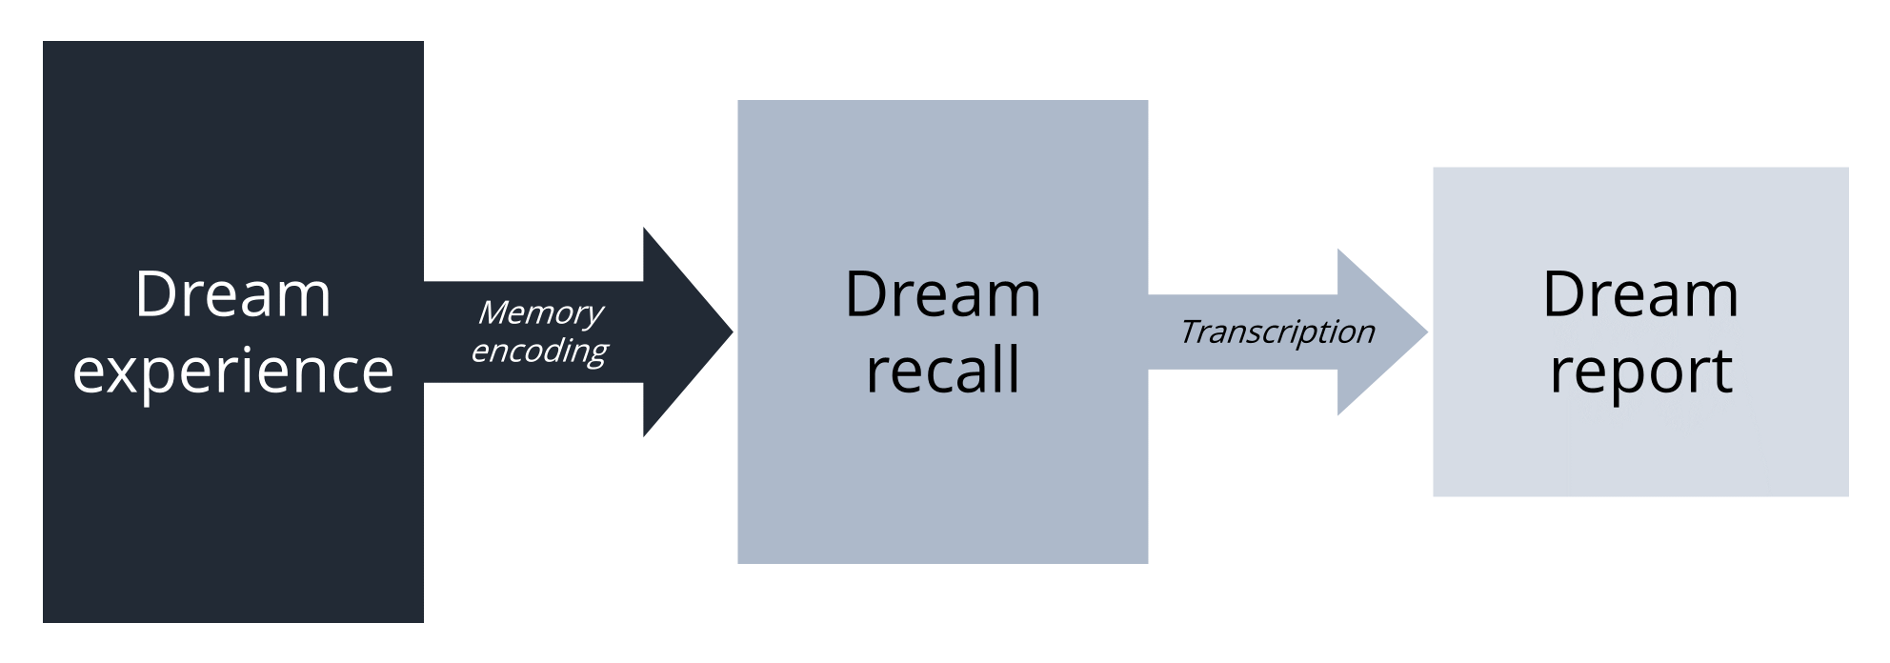
\includegraphics[width=\textwidth]{Fig/Intro/Intro_Guenole/Intro_Guenole.png}
	\caption[Guénolé's model of dreaming]{Guénolé's model of dreaming}
	\label{fig:intro:guenole}
\end{figure}

Because of this elusiveness of dreams and the constraints inherent to the scientific study of dreaming, it still remains one of the great mystery of the human cognition. Several questions on its nature and meaning are still not answered: do we dream every night? For how long? Why do we sometimes recall our dreams and sometimes not? Do dream reports obtained after awakening accurately convey subjective sleep experiences? What is, or what are, the function(s) of dreaming? What are the neurophysiological correlates of dreaming? The aim of the present thesis is to offer a modest contribution to the ongoing effort to solve these questions.

\section{Sleep}
\label{sec:dream-research:sleep}

As Schopenhauer rightly noticed, \q{the characteristic of dream is the condition of sleep peculiar to it}. Therefore, we cannot go any further in our study of dreaming without first defining the sleeping state and its physiology. Sleep is a normal physiological and periodic state characterized by vigilance suspension, which generally occurs during night time in humans. Sleep is a vital need that allows restoration of the immune, nervous, skeletal and muscular systems, leading some authors to postulate that \q{sleep is the price we pay for being alive} \citep{tononi_sleep_2014}. Long regarded as an idle state, it is becoming increasingly evident that sleep is \q{first and foremost a brain process} \citep{hirshkowitz_normal_2004} in which the brain is \q{hard at work and helps makes something of the world}, to borrow the words of Heraclitus’s famous aphorism (for an exhaustive review of the cognitive processes occurring during sleep, \citealt[see][]{andrillon_sleeping_2016}).

\subsection{Sleep stages}
\label{sec:dream-research:sleep:stages}

The invention of electro-encephalography (EEG) by Hans Berger in 1928 has paved the way for the scientific study of sleep. It was indeed soon after that discovery that Alfred Loomis first described a global slowing down of the brain rhythm during sleep, associated with the apparition of several grapho-elements such as K-complexes. Since then, sleep researchers have used EEG to monitor brain waves, electrooculography (EOG) to monitor eye movements and electromyography (EMG) to measure skeletal muscle activity. The simultaneous collection of these measurements is called polysomnography (PSG) and provides sufficient information to identify sleep stages according to standard international established guidelines. PSG is the gold standard in modern sleep science and is used in both clinical and research settings.

A first set of rules were published by Rechtschaffen and Kales (R\&K) in \citeyear{kales_manual_1968} and proposed to divide sleep into 5 stages with distinct electrophysiological properties, named rapid-eye movement (REM) and non-REM (NREM) stages 1, 2, 3, 4. This nomenclature was updated in 2007 by the American Academy of Sleep Medicine \citep{iber_aasm_2007} and sleep stage 3 and 4 have been merged into stage N3. Below are summarized EEG-EOG-EMG characteristics for wakefulness and the different sleep stages (see also Figure \ref{fig:intro:sleep_stage}).

\paragraph{Wakefulness}
Before diving into sleep, we first need to define the state of wakefulness. Eyes-closed quiet wakefulness is accompanied by an EEG rhythm predominantly in the alpha range (8-12 Hz). Opening the eyes or engaging in a significant mental task (for example mental calculation) reduces or blocks the alpha activity. Fairly high muscle activity can be present and slow or rapid eye movements may occur.

\paragraph{N1 sleep}
Stage N1 corresponds to the transitional period between wakefulness and sleep. The brain rhythm progressively decreases from alpha to theta (5 – 7 Hz), and the EOG is characterized by slow, rolling eye movements. N1 sleep represents approximatively 5\% of a normal night of sleep.

\paragraph{N2 sleep}
Each night, we spend more than half the night’s sleep in N2 sleep. The EEG activity during this stage is characterized by a predominance of theta waves, recurrently interrupted by two grapho-elements, the spindles and K-complexes, which are the landmarks of this sleep stage. K-complexes are defined as sharp negative waves followed by a positive component, prominent over frontal scalp electrodes and lasting more than 0.5 seconds. Spindles refer to burst of 12 to 14 Hz waves predominant over central scalp electrodes and lasting between 0.5 and 2 seconds. Beyond that, N2 sleep is characterized by an absence of eye movements as well as decreased muscle tone and brain metabolism.

\paragraph{N3 sleep}
N3 sleep, also referred to as deep sleep or slow-wave sleep, is the deepest sleep stage. It is characterized by a predominance (> 20\% of the epoch) of high amplitude (> 75 µV) delta waves (0.5 – 4 Hz). Eye motility, muscle tone and brain metabolism are even more decreased than in N2 sleep. N3 sleep represents approximatively 20\% of a normal night of sleep.

\paragraph{REM sleep}
As its name suggests, rapid eye movements (REM) sleep is characterized by rapid eye movements easily observable on the EOG channels. They consist of conjugate, irregular and sharply peaked eye movements, similar to some extent to those exhibited during wakefulness. Another fundamental aspect of REM sleep is its muscle atonia, as revealed by a low EMG activity. However, some transient muscle activity or muscle twitching (MTs) can also be observed. These short irregular bursts of EMG activity are superimposed on the background of low EMG activity. Brain metabolism is similar to that of wakefulness, and the EEG is marked by mixed low-amplitude waves predominantly in the theta band (saw-tooth waves), as well as a complete absence of delta rhythms. Other physiologic activities accompany REM sleep including middle ear muscle activity, periorbital integrated potentials, and sleep-related erections. REM sleep constitutes approximatively 20\% of a normal night of sleep.

\begin{figure}[htb]
	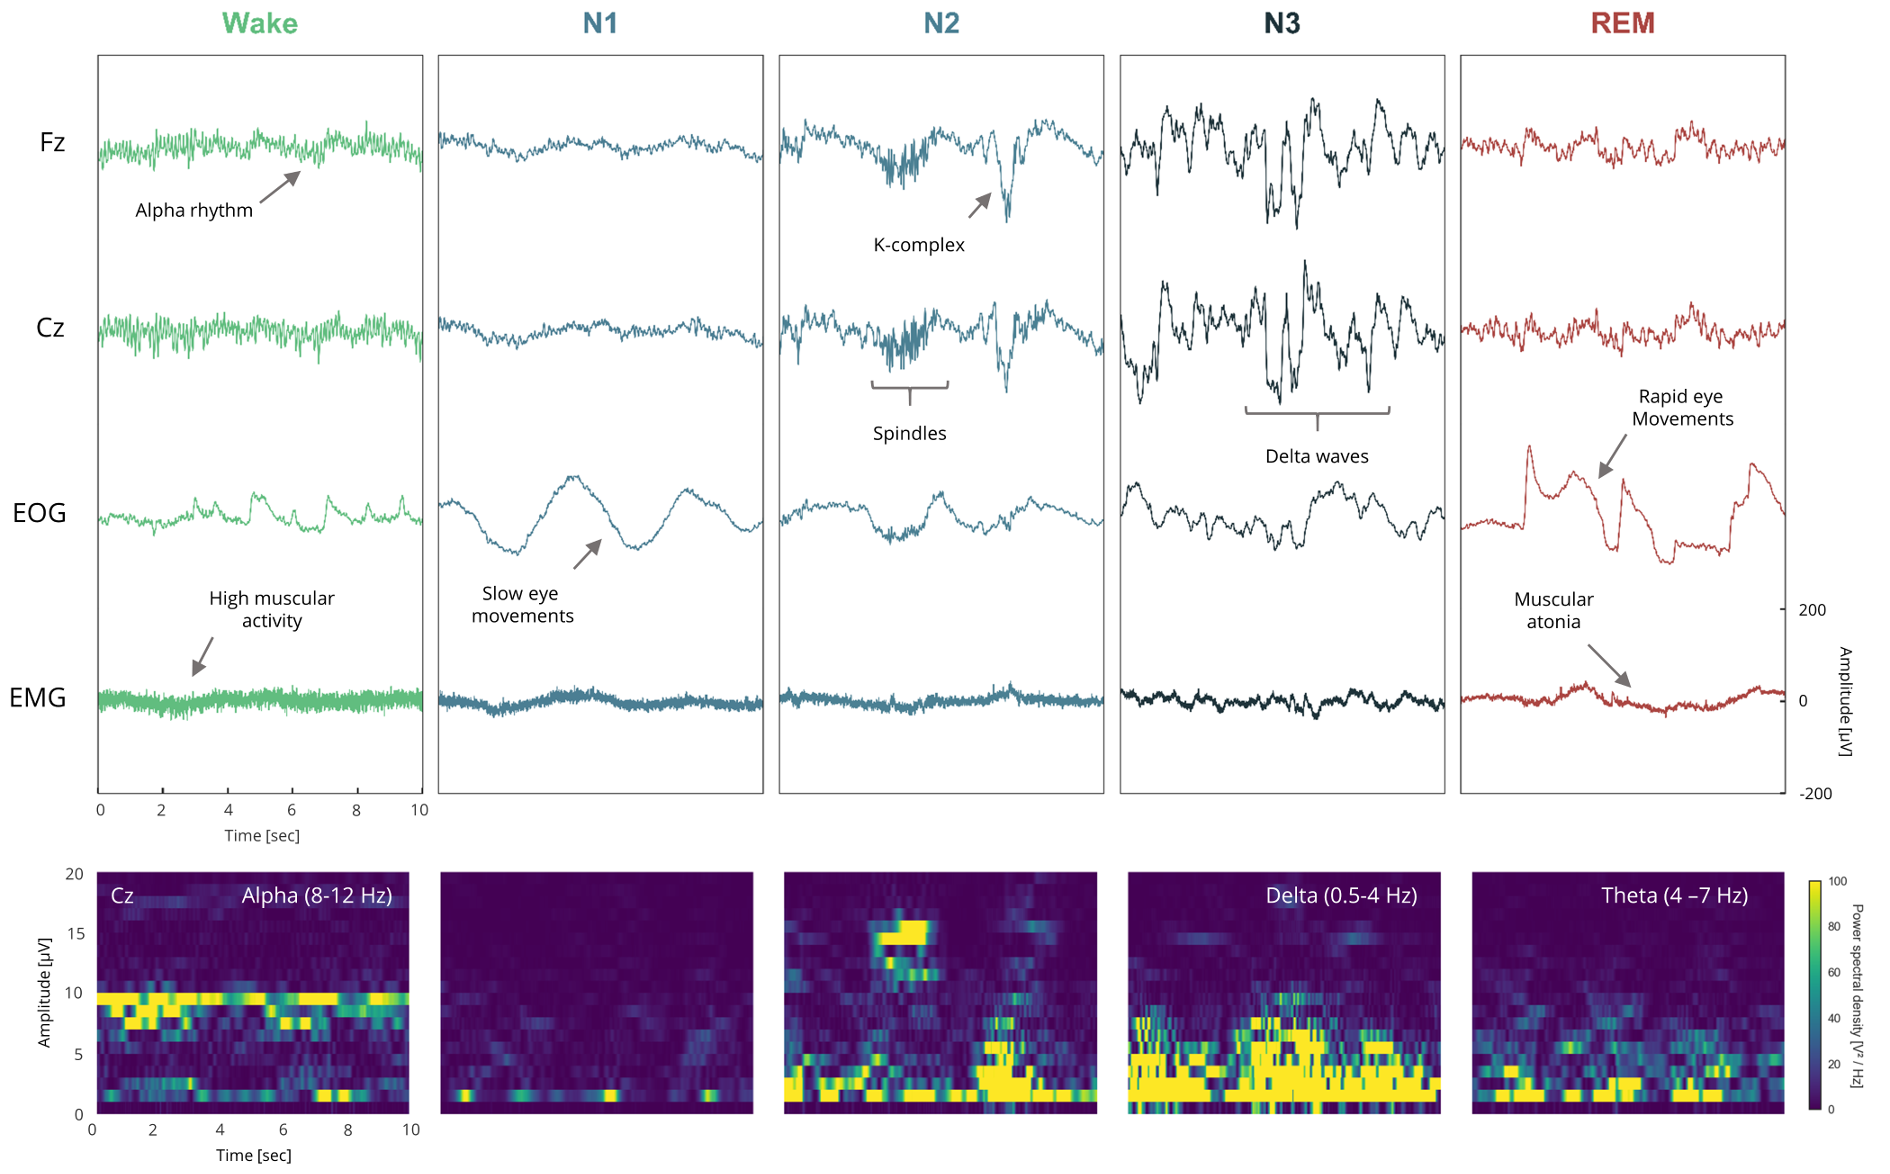
\includegraphics[width=\textwidth]{Fig/Intro/Intro_Sleep_Stages_PSD/Fig_Intro_Sleep_Stages_PSD_final_150517.png}
	\caption[Polysomnographic recordings across sleep and wakefulness]{Polysomnographic recordings across sleep and wakefulness. Top: Scalp EEG, EOG and EMG performed in one healthy young adult during wakefulness, N1, N2, N3 and REM sleep. The main features of each vigilance state are described. Bottom: Spectral properties of each stage obtained by computing the spectrogram of the Cz EEG signal atop.}
	\label{fig:intro:sleep_stage}
\end{figure}

\subsection{Sleep architecture}
\label{sec:dream-research:sleep:architecture}

Modern research has revealed that sleep is not a unitary, single block, but rather a cyclical succession of different brain states, which are all associated with specific functional roles. A normal night of sleep consists of a repetition of four or five 90 to 110 minutes long cycles in which sleep stages tend to follow each other in a particular order. The sleep cycle properties evolve with each cycle reoccurrence. Sleep staging is generally done visually by inspecting consecutive polysomnographic segments of 30 seconds. It results in a hypnogram which represents the succession of sleep stages across time (Figure 3). In his overview of the human sleep, Hirshkowitz described five generalizations about normal sleep architecture \citep{hirshkowitz_normal_2004}:

\begin{my_list_num}
    \item Sleep is entered through non-REM sleep
    \item Non-REM and REM sleep alternate approximately every 90 to 120 minutes
	\item N3 sleep predominates in the first third of the night
	\item REM sleep predominates in the last half of the night
	\item REM sleep occurs in four to six discrete episodes each night with episodes generally lengthening as sleep period progresses
\end{my_list_num}

\begin{figure}[htb]
	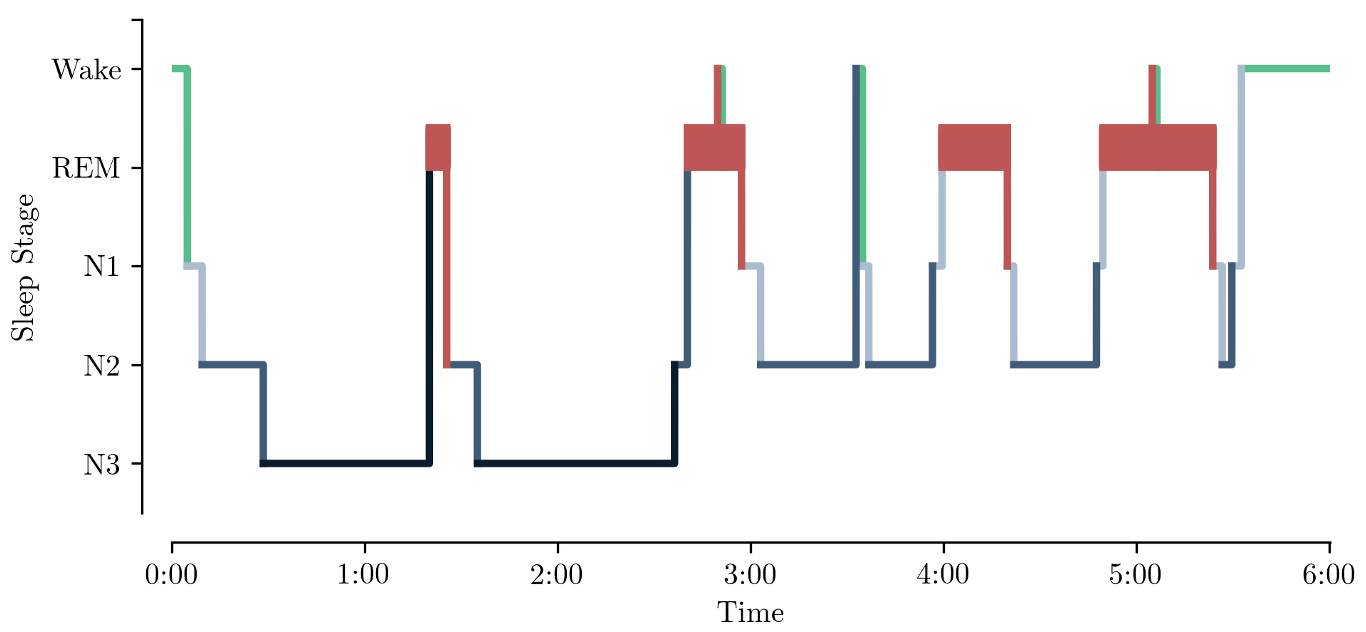
\includegraphics[width=\textwidth]{Fig/Intro/Intro_Hypnogram/Intro_Hypnogram.png}
	\caption[Example hypnogram of a healthy adult]{Example hypnogram of a healthy adult. The hypnogram is a graph which represents the stages of sleep as a function of time.One can easily recognize the succession of sleep cycles and especially the alternance of NREM (blue gradient) and REM sleep (red). Note that the hypnogram graph was generated directly as it is from the sleep software presented in the experimental results section.}
	\label{fig:intro:hypno}
\end{figure}

\section{Link between dreaming and sleep stages}
\label{sec:dream-research:link}

\subsection{The REM sleep hypothesis of dreaming}
\label{sec:dream-research:link:rem-sleep}

In the early fifties, Nathaniel Kleitman and his doctoral student Eugene Aserinsky, discovered in humans the existence of periods of sleep with an EEG similar to wakefulness (low voltage and fast frequencies), rapid eye movements and neurovegetative responses \citep{aserinsky_regularly_1953}. This discovery had a strong and persistent impact on dream and sleep research. The authors have indeed proposed that the rapid eye movements corresponded to the scanning of dream images. They reached this conclusion by comparing the proportion of dream reports obtained upon awakening in periods of eye motility and outside these periods, respectively 75\% and 11\% in their 1953’s study, and 80\% and 7\% in their 1957's study \citep{dement_relation_1957}. They concluded that their newly-discovered REM sleep stage was the neurophysiological basis of dreaming. A few years later, the French neurophysiologist Michel Jouvet, who had started working on sleep in cats, found that REM sleep was associated with muscular atonia \citep{jouvet_sur_1959}, a finding that was soon after replicated in humans \citep{berger_tonus_1961}. Pursuing his research on REM sleep, or \q{paradoxical sleep} as he named it, Jouvet had the idea to suppress the muscular atonia by injuring the brain stem of cats. To his astonishment, he found that the injured cats were performing, only during REM sleep, complex motor sequences, that he named \q{oneiric behavior} \citep{sastre_comportement_1979}. For him and the scientific community at the time, it was clear that these motors sequences were directly related to the cat's dreams, and this experiment provided a significant evidence in favor of the REM sleep hypothesis of dreaming.

However, even though equating dreaming with REM sleep provided a useful way to scientifically explore dreaming, it soon became apparent that dreaming was in fact not exclusively present during REM sleep but also during all the other sleep stages. Few years after the initial discovery of REM sleep, several researchers reported a much higher proportion of dream report in non-REM sleep than what was expected based on the findings of the Kleitman’s team \citep{goodenough_comparison_1959, foulkes_dream_1962}. Comparing the recall rate of people who never remembered their dreams with people who frequently recalled them, Goodenough and colleagues found respectively 34\% and 54\% of dream reports outside of REM sleep. The recall rate went up to 54\% in Foulkes’s study which comprised 200 awakenings. Since then, numerous studies have replicated the finding of mentation outside of REM sleep \citep{nielsen_review_2000}, even in the periods of non-REM sleep located before the first nocturnal episode of REM sleep \citep{noreika_early-night_2009}. As a counterpoint, it has become apparent that a significant proportion (~15\%) of REM sleep awakenings were not followed by a dream report. It results that dreaming is not specific of REM sleep.

Despite the REM sleep hypothesis of dreaming is still present in the public mind, the occurrence of dream mentation in all sleep stages is increasingly accepted in the scientific community. As Schwartz and colleagues aptly pointed out, \q{REM sleep is not a necessary, but a facilitating condition for dreaming to occur. Conversely, there is little doubt that dreaming was a necessary condition for REM sleep to become famous} \citep{schwartz_dreaming:_2005}.

\subsection{The fore-brain hypothesis of dreaming}
\label{sec:dream-research:link:solms}

Equating dreaming with REM sleep, Hobson argued that dreaming depends on the brainstem REM sleep generator \citep{hobson_dream_1998}. This was the dominant theory for several decades until a firm opponent of the REM sleep hypothesis of dreaming, Mark Solms, refuted it using neuropsychological evidences. He examined 361 neurological patients and asked them in detail about their dreaming \cite{solms_neuropsychology_1997}. He found that out of 26 case reports of REM sleep loss or alteration following a lesion in the brainstem (Pons area), 25 were not associated with subsequent alterations in dream reporting. By contrast, he reported that in most cases global cessation of dreaming (a condition referred to as the Charcot-Wilbrand syndrome) followed lesions in or near the temporo-parietal junction (TPJ) and the medial prefrontal cortex (MPFC; see Figure \ref{fig:intro:lesions}). Importantly, damage in these two regions were rarely associated with REM sleep disturbances. This double dissociation provides a clear argument that not only dreaming can occur outside of REM sleep, but it is also not dependent of the brainstem generators of REM sleep. This led Solms to put forward the fore-brain hypothesis of dreaming, which proposes that dreaming is controlled through forebrain mechanisms involving at least TPJ and MPFC.

\begin{figure}[htb]
	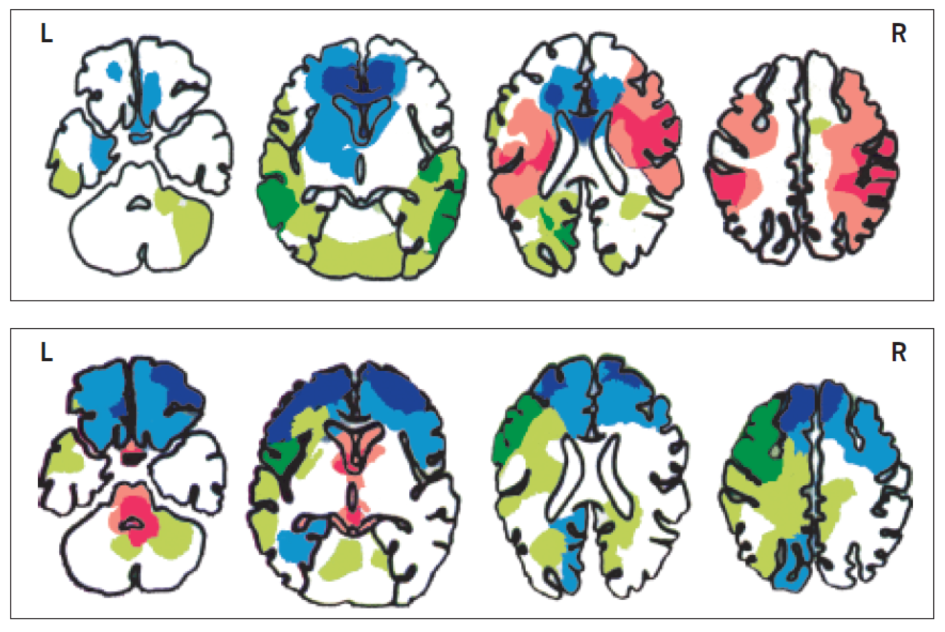
\includegraphics[width=\textwidth]{Fig/Intro/Intro_Lesions/Intro_Lesions.png}
	\caption[Lesion maps associated with cessation vs preservation of dreaming]{Lesion maps associated with cessation vs preservation of dreaming. Top: Global cessation of dreaming was found following parietal lobe lesions (6 cases, inferior lobule and supramarginal gyrus; red), medial frontal lesions (9 cases; blue), and posterior lesions (8 cases; green). Bottom: Preserved dreaming was found following left hemispheric and frontal convexity lesions (15 cases; green), bifrontal lesions (14 cases; blue), and brainstem lesions (17 cases; red). Reproduced from \citet{schwartz_dreaming:_2005}}
	\label{fig:intro:lesions}
\end{figure}

\subsection{A continuum of mentation during sleep}
\label{sec:dream-research:link:continuum}

Based on Solms’s findings, some authors have postulated that instead of relying on REM sleep mechanisms, dreaming might be best described along a \q{continuum} of mentation during sleep, ranging from the hypnagogic reveries typical of sleep onset to florid and vivid dreamlike experiences typical during REM sleep \citep{schwartz_dreaming:_2005}. A brief description of this continuum of mental activities during sleep is reported in Table \ref{tab:intro:continuum}.

% Please add the following required packages to your document preamble:

\begin{table}[htb]
\caption[A continuum of sleep mentation]{A brief description of sleep mentation in their typical order of placement during the sleep cycle. Modified from \citet{de_koninck_sleep_2012}}
\label{tab:intro:continuum}
\resizebox{\textwidth}{!}{%
\begin{tabularx}{\textwidth}{XXX}
\toprule
\textbf{Name}                                                         & \textbf{Description}                                                                          & \textbf{Sleep stage}                         \\ \midrule
Hypnagogic reverie                                                    & Simple images                                                                                 & Sleep onset mentation (N1 or early N2 sleep) \\
Reflections                                                           & Thoughts with no hallucinatory content                                                        & N2 sleep                                     \\
Vivid dreams                                                          & Vivid imagery and sequences, presence of characters, interactions and emotions                & REM and NREM sleep                           \\
Lucid dreams                                                          & The dreamer is conscious of dreaming and can sometimes controls the dream scenario            & REM sleep                                    \\
Nightmares and bad dreams 	  										  & Unpleasant and highly anxiogenic dream. The content of nightmare actually awakens the dreamer & REM sleep                                    \\
Hypnopompic reverie                                                   & Characterized by elaborate imagery                                                            & Sleep offset mentation (REM or NREM sleep)   \\ \bottomrule
\end{tabularx}%
}
\end{table}


\section{Attempts to study the cerebral correlates of dreaming}
\label{sec:dream-research:attempts}

Thanks to the recent advances in neuroimaging techniques, we have the means to measure, with unprecedented spatial and temporal accuracy, what is happening in the brain at a specific moment in time (see Methods section). Yet, since it is now well-accepted that dreaming can occur in all sleep stages, and because dream consciousness is only accessible via report rather than direct observation, it is therefore impossible to be sure that dreaming is happening at a specific time point during sleep. This conceptual issue has not prevented sleep and dream researchers to attempt to identify the cerebral correlates of dreaming. The main methods and findings are summarized in the following paragraphs.

\subsection{Brain activity during REM sleep}
\label{sec:dream-research:attempts:ba-rem}

On the basis of the REM sleep hypothesis of dreaming, which was predominant during the nineties, researchers used functional neuroimaging techniques such as positron emission tomography (PET) to investigate the brain activity during REM sleep. They reported that, despite strong similarities between the wake and REM sleep electrophysiological scalp signals, the brain metabolism in these two vigilance states was disparate \citep{maquet_functional_1996, braun_regional_1997}. Among the most notable findings, the regional cerebral blood flow (rCBF) was decreased in several brain regions including the dorsolateral prefrontal cortex (DLPFC), and was increased in other regions (occipital, temporal, and superior parietal cortices, hippocampal formation, anterior cingulate and the pons). Following these works, researchers postulated that these changes in the brain functional organization could explain the phenomenological characteristics of dream reports \citep{hobson_dreaming_2000, nir_dreaming_2010}. For instance, increased occipital cortex activity during REM sleep could explain the clear predominance of visual modality in dream reports, a phenomenon that Vincent van Gogh had already noticed when he wrote: \q{I often think that the night is more alive and more richly colored than the day} (Vincent van Gogh, 1888). Second, the increased activity during REM sleep in the hippocampal formation, a region well-known for its role in memory encoding and retrieval, could account for the presence of known images and characters in dreams. Finally, the decreased activity in the dorsolateral prefrontal cortex, a region involved in executive function, cognitive control and working memory, could account for the lack of consistency, voluntary control and logical reasoning over the dream story. This is consistent with studies on lucid dreaming which showed a partial reactivation of this area in lucid dreams compared to non-lucid dreams. We will return to these correspondences between the phenomenology of dreams and brain activity in the chapter on the default mode network.

\subsection{Brain activity during lucid dreaming}
\label{sec:dream-research:attempts:ba-lucid}

Long considered as a fantasy, lucid dreaming - the ability to become self-aware of dreaming during a dream, and in some cases, to control the dream scenario – has recently gained considerable interest among researchers and the public. The scientific study of lucid dreaming started in the nineteenth century when Hervey de Saint Denys, a learned oneirologist, published his landmark book \q{Dreams and the Ways to Direct Them: Practical Observations}, in which he described his own lucid dream experiences. More than a century later, more objective methods such as EEG and functional magnetic resonance imaging (fMRI) have become the technique of choice for understanding lucid dreams. Using a pre-determined ocular signal, Dresler was remarkably able to measure, in real-time, the brain activity during lucid REM sleep and non-lucid REM sleep (though only one subject out of four had lucid dreams of sufficient length; \citet{dresler_neural_2012}). Lucid REM sleep was associated with a reactivation of areas that are normally deactivated during REM sleep, such as bilateral precuneous, parietal lobules and prefrontal and occipito-temporal cortices. Phenomenologically, these regions are either involved in self-awareness and executive functions, and their reactivation during lucid dreaming could account for the resurgence of a certain level of self-awareness and voluntary control. Even more recently, Voss was able to induce self-reflective awareness during dream using fronto-temporal transcranial alternating current stimulation \citep{voss_induction_2014}. They reported that lucid dreams were most prominent during stimulation in the lower gamma band (58\% of lucid dreams following a stimulation at 25 Hz and 77\% of lucid dreams following a stimulation at 40 Hz). However, the lucidity was not assessed directly by the dreamer but assumed a posteriori if the subjects reported elevated ratings on a lucidity scale. In conclusion, lucid dreaming provides an appealing and elegant way to study, in real time, the cerebral correlates of dreaming. Yet, the inherent problem with this method lies precisely in the fact that lucid dreams are, by nature, different from non-lucid dreams. As exciting as the results are, it would be however difficult to generalize them to the research on non-lucid dreams.

\subsection{Brain activity in the minutes preceding a dream report}
\label{sec:dream-research:attempts:ba-pre}

Another line of research consists in comparing the EEG power in various frequency bands in the minutes preceding a morning awakening associated, or not, with a dream recall. This paradigm has been used in several studies over the last decades, the findings of which are summarized as follows.

\citet{esposito_reduced_2004} reported that in both REM and N2 sleep, dream recall was associated with a lower alpha and delta power in the 3 minutes preceding awakening. According to the authors, the alpha effect may reflect increased cognitive elaboration and visual imagery as well as increased attention and memory processes. A few years later, \citet{marzano_recalling_2011} found that dream recall after morning awakening from REM sleep was associated with a higher frontal 5–7 Hz (theta) activity in the 5 minutes preceding awakening. In N2 sleep, dream recall was associated with a decrease in alpha power, an observation consistent with Esposito’s results. The same year, another study reported a lower delta power for the dream recall condition following awakening from N2 sleep, and a higher alpha and beta power in occipital derivations for REM sleep \citep{chellappa_cortical_2011}. Finally, a recent study, inaccurately entitled \q{the cerebral correlates of dreaming}, reported that in both N2 and REM sleep, reports of dream experience were associated with local decreases in delta power in posterior cortical regions in the 2 minutes preceding awakening \citep{siclari_neural_2017}. The authors were able to predict whether an individual reported dreaming or the absence of dream experiences after awakening from N2 sleep by monitoring this posterior ‘hot zone’ in real time.
The results from these studies are heterogeneous and sometimes contradictory. Moreover, despite this paradigm may seem attractive at first, the problem still remains that we can never be sure whether the dream actually took place in the minutes just before awakening or several tens of minutes before.

\subsection{Dreaming as a subsystem of the default mode network}
\label{sec:dream-research:attempts:dmn}

The past few years have witnessed the emergence of a new conceptual framework of dreaming, centered on the idea that dreaming is a unique form of mind-wandering, which cerebral correlates are a subsystem of the default mode network (DMN; see Methods section; \citealp{maquet_human_2005, domhoff_neural_2011, domhoff_dreaming_2015, christoff_mind-wandering_2016}). Based on the fact that dreaming and waking spontaneous thought share many features (i.e. predominance of the audiovisual modalities, centered on one’s current goals and concerns, draw heavily on semantic and episodic memory in constructing simulations and future plans, presence of a wide range of affect), some authors have postulated that dreaming is a \q{type of spontaneous thought that is highly unconstrained, hyper-associative and highly immersive} \citep{christoff_mind-wandering_2016}. Using the results of lesion and REM sleep neuroimaging studies, they argued that dreaming should be accompanied, at the neural level, by a strong recruitment of the default mode network medial temporal lobe (MTL)-centered subsystem and strong deactivations in frontoparietal control network regions (such as the DLPFC). Activation of the former areas could be related to the generation of spontaneous thoughts, during both wake and sleep, while the deactivation of the latter areas could explain the high volatility and variability of dream content over time.

\cleardoublepage

\chapter{Dream recall frequency}
\label{sec:dream-recall}

\cleanchapterquote{We must also inquire what the dream is, and from what cause sleepers sometimes dream, and sometimes do not; or whether the truth is that sleepers always dream but do not always remember (their dream); and if this occurs, what its explanation is.}{Aristotle}{On dreams. 350 B.C.}

\section{Measuring dream recall frequency}
\label{sec:dream-recall:method}

As Aristotle had rightly pointed out, we do not always remember our dreams. More than two thousand years after, modern research has confirmed that the dream recall frequency (DRF) – i.e. the number of dream reports over a given period of time - is indeed highly variable both within individuals over the life course, but also between individuals \citep{schredl_factors_2003, ruby_experimental_2011}.

There is no gold standard for measuring DRF, and each method has its pros and cons. In research settings, three methods are commonly applied: questionnaire scales, dream diaries, and laboratory awakenings \citep{schredl_dream_1999}. The former consists in asking the participants to estimate their dream recall frequency over the last few weeks or months. This method has the advantage of being fast, inexpensive, and unaffected by the measurement, however, the DRF could be over- or under-estimated due to erroneous or incomplete recollection. Regarding dream diaries, the participants are asked to report each morning whether they have recalled a dream or not. This method minimizes the bias of retrospective estimation, but has the disadvantages of potentially increasing drastically the dream recall frequency, especially in persons who usually almost never recall their dreams \citep{schredl_questionnaires_2002}. Finally, laboratory awakenings consist in awakening the participants in the sleep lab and asking them whether they recall a dream or not. While this method has the clear advantage that the experimenters can measure physiological parameters (EEG, EOG, ECG, respiration and heart rate) prior, during and after the awakening, it is also time-consuming and expensive. Moreover, as for dream diaries, laboratory awakenings are associated with a dramatic increase in DRF, especially for low dream recallers.

\section{DRF in the general population}
\label{sec:dream-recall:pop}

\subsection{Average DRF}
\label{sec:dream-recall:pop:avg}

Measured by questionnaire, the average weekly DRF was 2.58 ± 2.03 in 444 German students \citep{schredl_factors_2003} and 0.83 ± 1.57 in a representative German sample of 931 participants \citep{schredl_dream_2008}. Using dream diaries, the average weekly DRF was 3.1 ± 1.5 in 70 Finnish children \citep{valli_threat_2005} and 3.9 ± 2.5 in a sample of 196 German student \citep{schredl_reliability_2005}. In lights of these results, we can conclude that the average weekly DRF in the general population lies between 1 and 3 dream reports per week.

\subsection{Intra-individuals variability}
\label{sec:dream-recall:pop:intra}

Daily experience suggest that our ability to recall dream fluctuate over time. Investigating this issue using the diary technique in 169 participants, \citet{schredl_reliability_2005} reported that the stability of DRF was very high over a period of one month. Similarly, he reported high DRF stability coefficients in a sample of older adults who had been interviewed weekly about their dream life over a period of 26 weeks \citep{schredl_reliability_2001}. However, to our knowledge, there are no studies evaluating the stability of DRF in the same individuals over an extended period of time.

\subsection{Inter-individuals variability}
\label{sec:dream-recall:pop:inter}

DRF varies drastically between individuals: some persons almost never recall a dream, whereas others can recall one or several dreams every morning. In an Austrian sample of 1000 persons, \citet{stepansky_austrian_1998} found that 31\% of the participants reported 10 dreams or more per month, 37\% reported between one and nine dreams per month, and 32\% reported less than one dream per month. In a sample of 285 German students, \citet{schredl_questionnaires_2002} found that 44\% reported dreams four or more times per weeks, 44\% reported a dream one time per week and 12\% reported a dream less than one time per month. This variability allows to differentiate behavioral profiles of DRF: high dream recallers (HR), who can recall a dream almost every morning (e.g. more than 5 mornings a week, \citealp{schredl_reliability_2005}) and low dream recallers (LR), who almost never recall a dream (e.g. less than one dream per month, \citealp{goodenough_comparison_1959}). Importantly, the frequency of HR is higher in the general population, and even more in young and/or student sample \citep{schredl_reliability_2005}.

\section{Parameters correlated with DRF}
\label{sec:dream-recall:param}

\subsection{Physiological and psychological factors}
\label{sec:dream-recall:param:psych}

First, increased professional or personal stress is positively associated with DRF \citep{schredl_dream_1999}. Similarly, an interest in dreams, or a positive attitude towards dreams is positively associated with DRF, as is frequent day-dreaming and rich fantasy life \citep{schredl_factors_2003}. DRF decreases with age and is slightly higher in women, who are also typically more interested in dreams \citep{schredl_dream_2008, schredl_gender_2008}. Regarding personality dimensions, studies have found positive correlations between DRF and thin boundaries, anxiety, and openness to experience \citep{hartmann_boundaries_1989, schredl_factors_2003,schredl_dream_2003}. However, most of the correlations between DRF and personality traits are low and explain only a small percentage of the total variance.

\subsection{Cognitive factors}
\label{sec:dream-recall:param:cogn}

Regarding cognitive abilities, a simple explanation of why individuals differ in their ability to remember dreams could be because they differ in some more general memory abilities (verbal, visual, short and long term). However, the literature yielded contradictory results, with some support for a positive association between DRF and visual memory, but also evidence against it for verbal and visual material and short-or long-term story narrative recall \citep{ruby_experimental_2011, blagrove_trait_2010}. On another note, several studies have consistently reported that DRF is positively correlated with creativity \citep{fitch_variations_1989, schredl_creativity_1995, schredl_factors_2003} and intelligence scales (multiple-choice vocabulary test, \citealp{schonbar_manifest_1959}, Shipley-Hartford intelligence scale, \citealp{connor_reported_1970}).

\subsection{Sleep parameters}
\label{sec:dream-recall:param:sleep}

First, DRF varies according to the sleep stage preceding awakening (see \citealp{nielsen_review_2000} for a review). More dream reports are obtained after an awakening during REM sleep than after an awakening during NREM sleep. These results inspired the REM sleep hypothesis of dreaming discussed earlier in section \ref{sec:dream-research:link:rem-sleep}. However, when a dream is not reported on awakening, there is no method of establishing whether it did not happen or was forgotten. This idea was rightly pointed out by \citet{conduit_poor_2004}: \q{An ongoing assumption made by sleep scientists is that since dreams are more often recalled on awakening from REM sleep, dreams must occur more often during this sleep stage. An alternative hypothesis is that cognition occurs throughout sleep, but the recall of mentation differs on awakenings}.

This idea that DRF variability is not a matter of dream production during sleep, but of dream recall during awakening, is the core of several models of dream recall (detailed later in section \ref{sec:dream-recall:theories}), among which the arousal-retrieval model is one of the most significant. In its simplest form, it claims that a period of wakefulness must occur just after dreaming so that the dream content can be transferred from short term to long term memory \citep{koulack_dream_1976}
Several studies support this model. First, using retrospective evaluation, \citet{schredl_factors_2003} found a positive correlation between the number of nocturnal awakenings and DRF. Second, \citet{de_gennaro_recovery_2010} reported that recovery sleep following a full night of sleep deprivation was characterized by an almost complete abolition of dream recall, paralleled with a lower number of nocturnal awakenings, which could, according to them, have \q{reduced the contents available in memory as possible cues for retrieval of dream experiences at morning}. Finally, these results were recently reinforced by a full-night PSG study in 36 subjects (18 HR and 18 LR; \citealp{eichenlaub_brain_2014}; Figure \ref{fig:intro:jbe-sleep}). HR showed in average longer intra-sleep wakefulness than LR (30 min vs 15 on average). The number of awakenings (the number of phases composed of consecutive pages of awakening) was not significantly different between the 2 groups, but the mean duration of the awakenings was (HR, 1.90 ± 0.91 min; LR, 0.95 ± 0.40 min).

\begin{figure}[htb]
	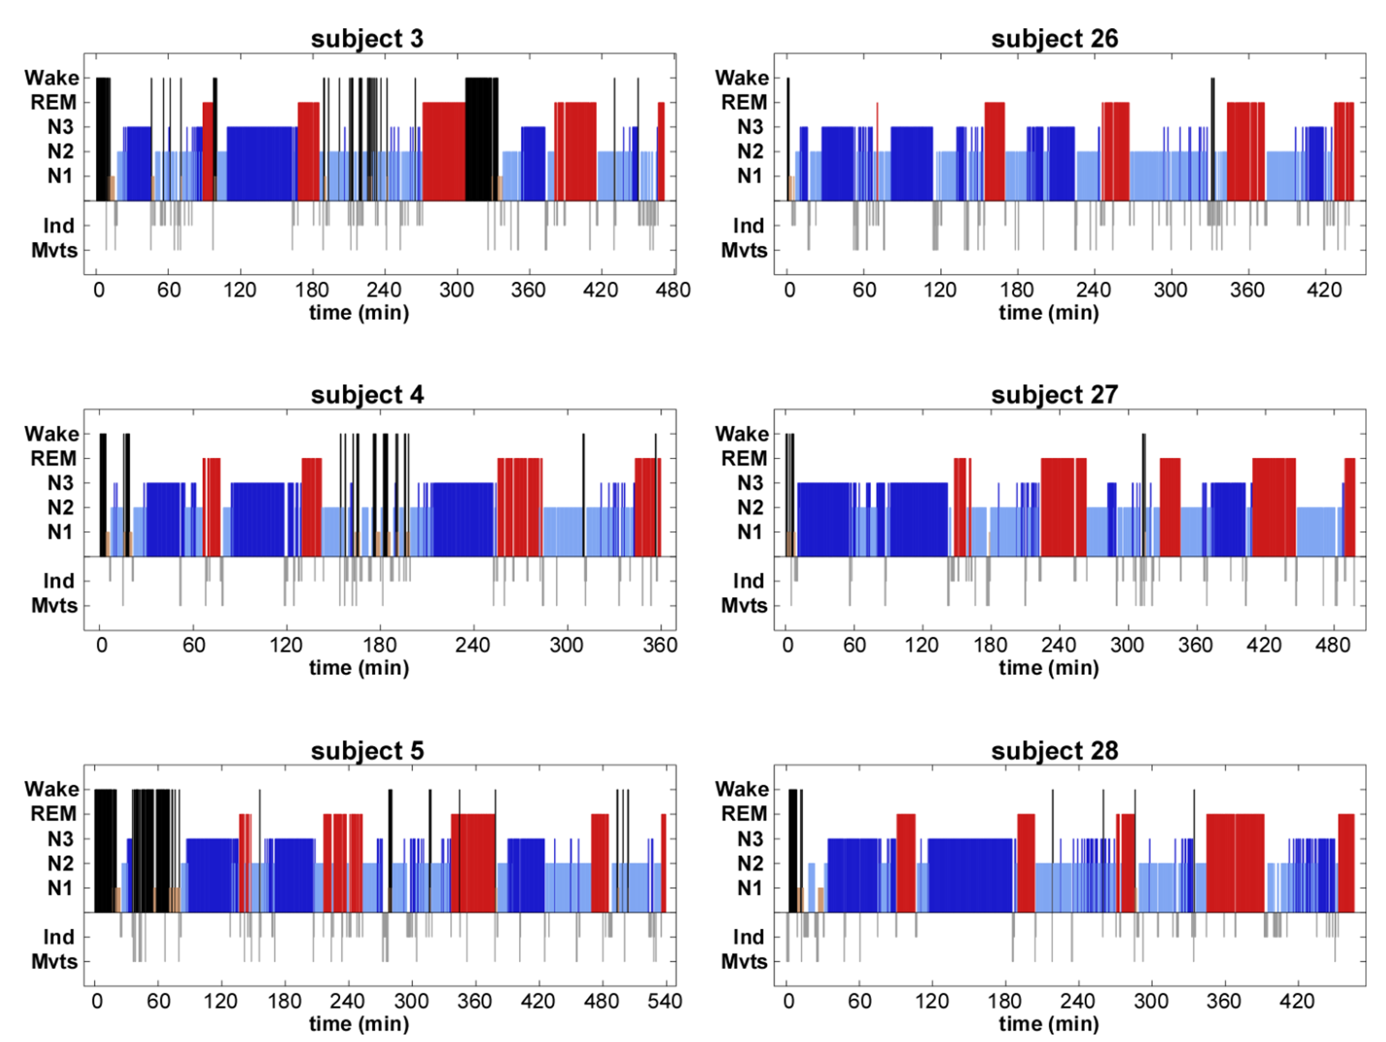
\includegraphics[width=\textwidth]{Fig/Intro/Intro_JBE_sleep/Intro_JBE_sleep.png}
	\caption[Hypnograms of typical high and low dream recallers]{\textbf{Hypnograms of three representative HR (left) and three representative LR (right).} Full night PSG recordings were acquired in the sleep lab in 18 HRs and 18 LRs. Wake: wakefulness (black); N1, N2, and N3: sleep stages N1 (very light gray), N2 (light gray), and N3 (dark gray), respectively; REM: REM sleep (medium gray); Ind: pages for which the dominant sleep stage could not be determined; Mvts: movements. From these 6 examples, it can be observed that the wakefulness periods during the sleep period time are longer in HR than in LR. Adapted from \citet{eichenlaub_brain_2014}}
	\label{fig:intro:jbe-sleep}
\end{figure}

\subsection{Neurophysiological parameters}
\label{sec:dream-recall:param:neuro}

The neurophysiological parameters that covary with DRF had never been investigated until the doctoral work of Jean-Baptiste Eichenlaub, conducted with Perrine Ruby a few years ago. They compared the brain activity of HR and LR during both sleep and wakefulness and using several neuroimaging techniques such as auditory evoked potentials (AEP) and positron emission tomography (PET). The main findings from Eichenlaub’s doctoral thesis are summarized in Figure \ref{fig:intro:jbe-summary}.
First, they conducted a sleep lab study in which they compared the brain reactivity (AEP) of 18 HRs (DRF = 4.4 ± 1.0 dream reports per week) and 18 LRs (0.25 ± 0.1) during sleep and wakefulness \citep{ruby_alpha_2013, eichenlaub_brain_2014}. During data acquisition, the subjects were presented with sounds to be ignored (first names randomly presented among pure tones) while they were watching a silent movie or sleeping. They found that brain responses to first names dramatically differed between the 2 groups during both sleep and wakefulness (Figure \ref{fig:intro:jbe-summary}A). During wakefulness, the attention-orienting brain response (P3a) and a late parietal response were larger in HR than in LR. During sleep, there were between-group differences at the latency of the P3a during N2 sleep and at later latencies during all sleep stages.
Second, they used PET to compare the resting state cerebral blood flow of 21 HRs (DRF = 5.2 ± 1.4 dream reports per week) and 20 LRs (DRF = 0.5 ± 0.3 dream reports per week) during sleep and wakefulness \citep{eichenlaub_resting_2014}. Compared with LRs, HRs showed higher rCBF in the TPJ during REM sleep, N3, and wakefulness, and in the MPFC during REM sleep and wakefulness (Figure \ref{fig:intro:jbe-summary}B).
Altogether, these findings show that HR and LR have different neurophysiological traits: spontaneous and evoked brain activity of HR and LR differ during wakefulness and sleep. They argued that HR’s neurophysiological profile could promote mental imagery during sleep and the encoding or retrieval of the dream memory during wakefulness. Notably, increased attention-orienting responses during sleep in HR could promote intra-sleep awakenings, which in turn would facilitate the encoding of dreams according to the arousal-retrieval model, and finally result in a higher likelihood of dream recall in the morning after awakening.

\begin{figure}[!htb]
	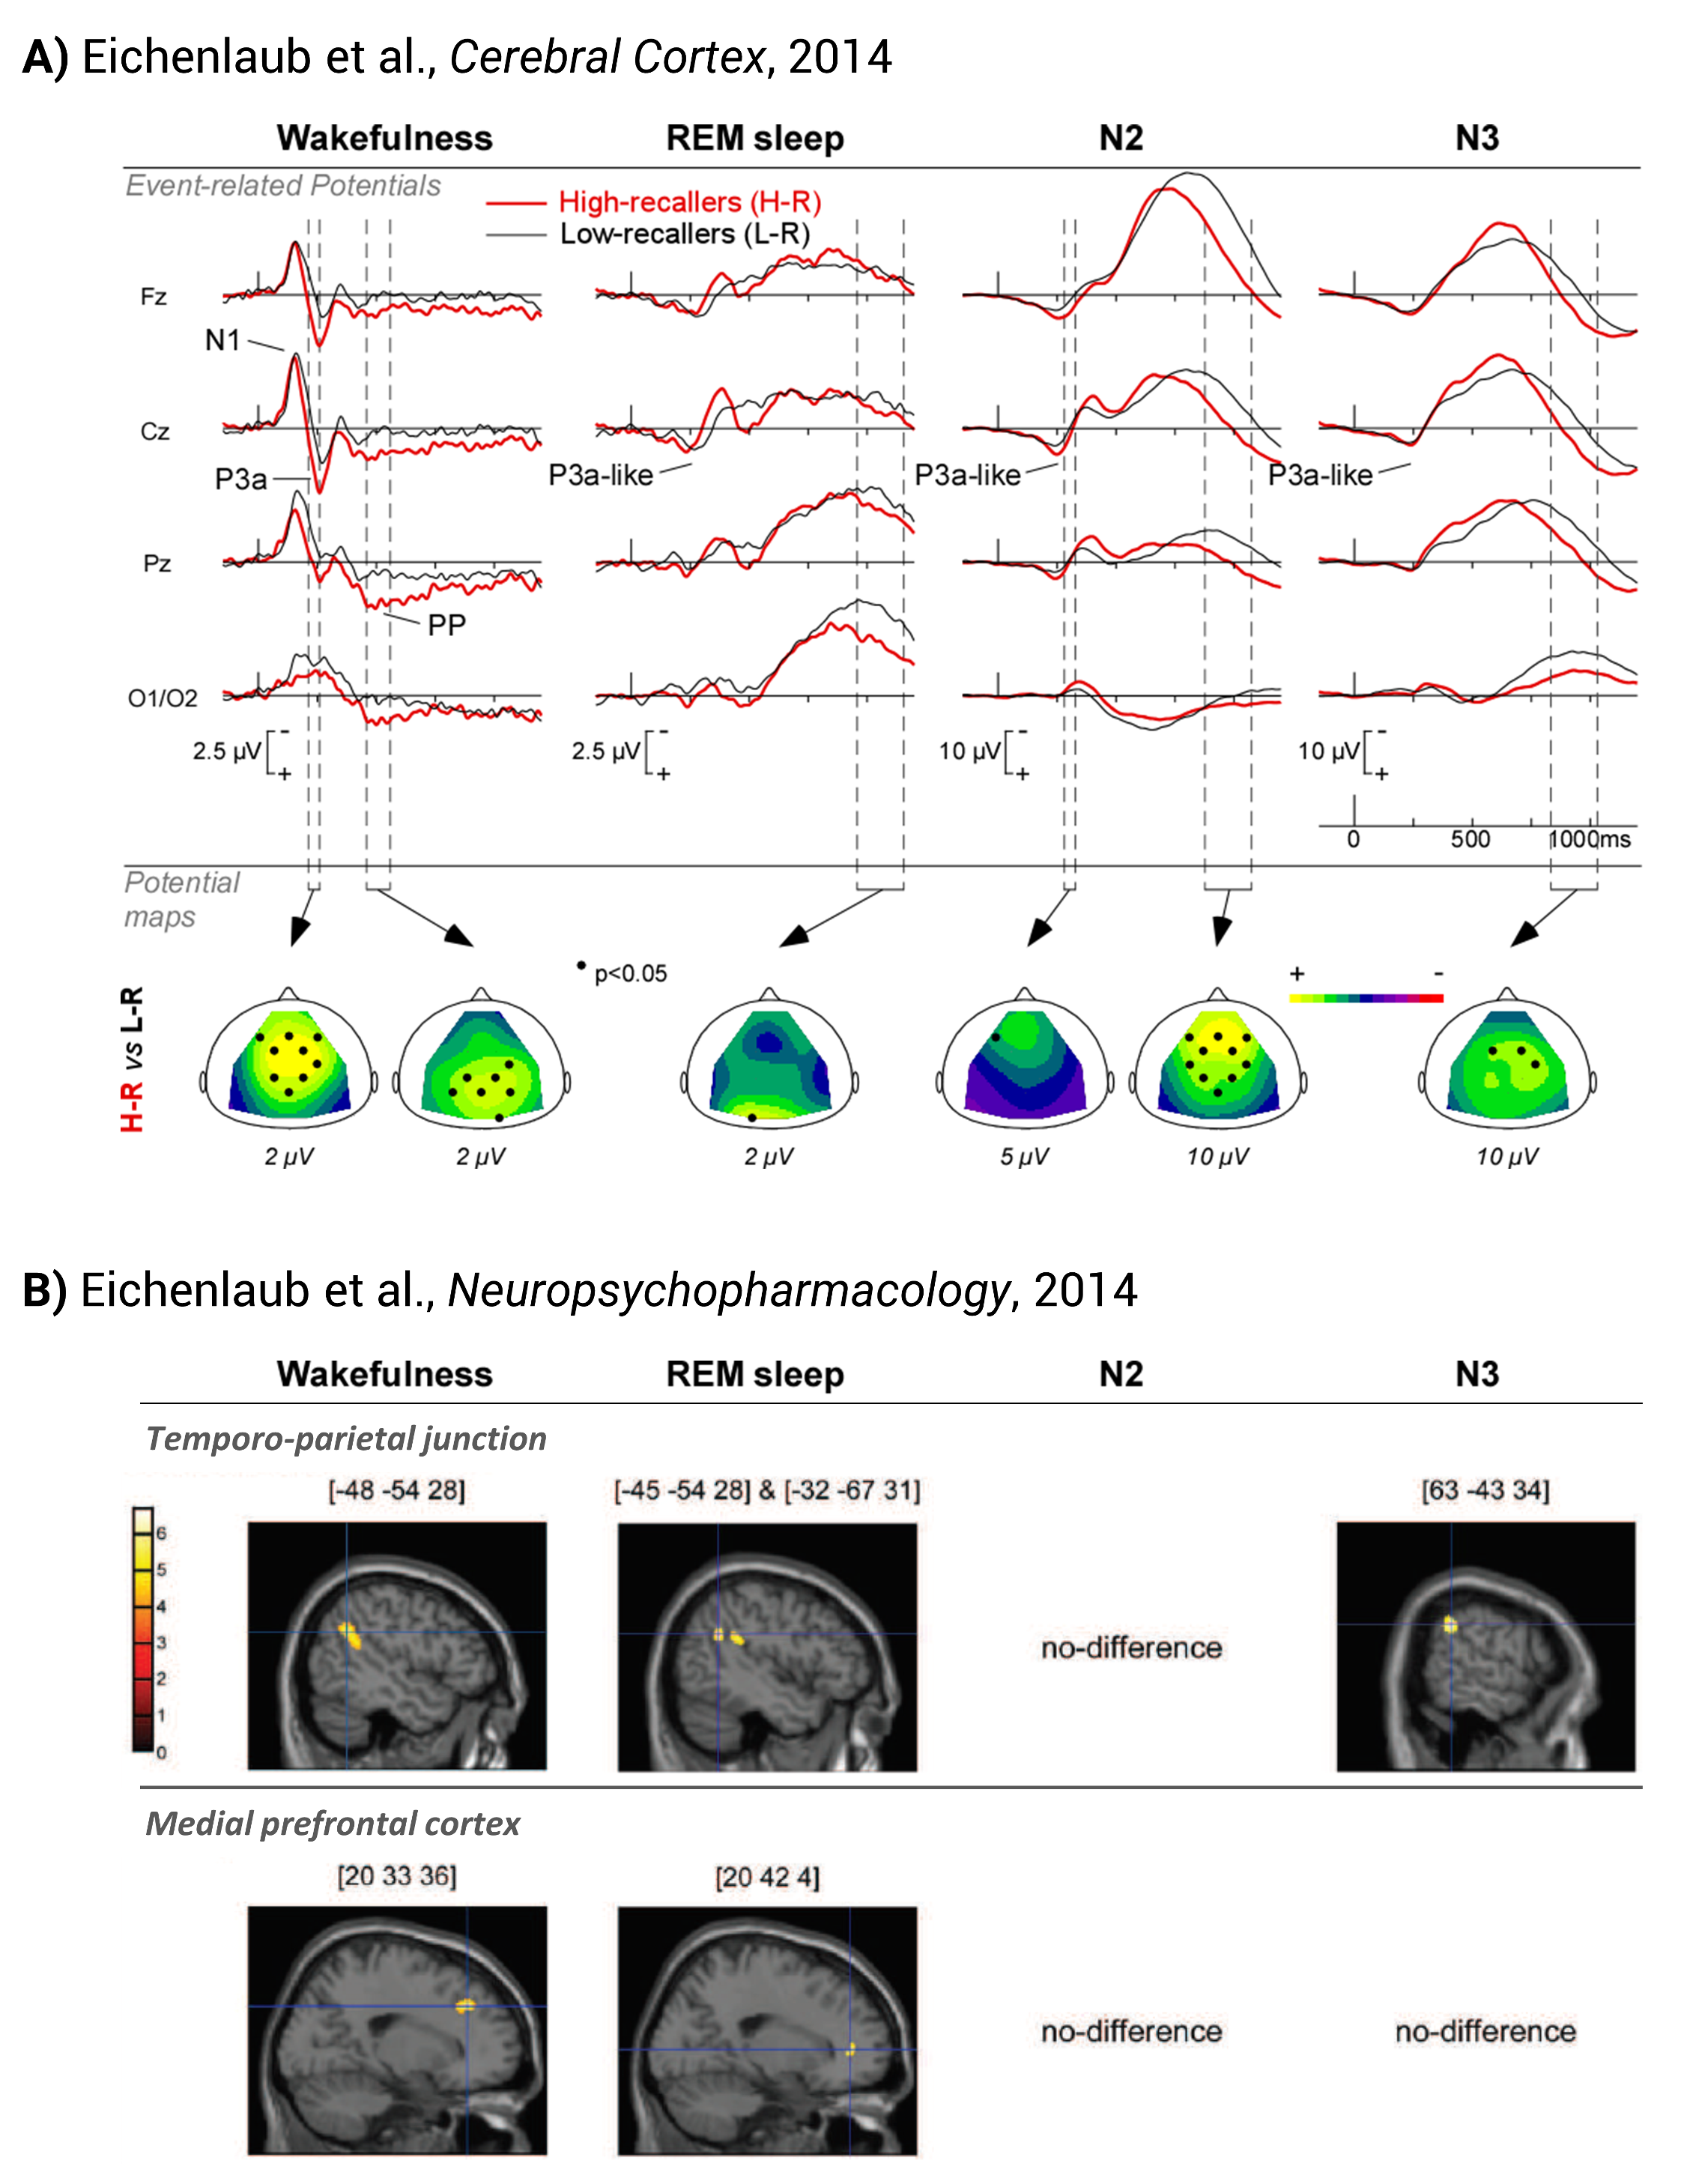
\includegraphics[width=\textwidth]{Fig/Intro/Intro_JBE_summary/Intro_JBE_summary.png}
	\caption[Summary of the results obtained in Eichenlaub's PhD thesis]{\textbf{Summary of the results obtained in Eichenlaub's PhD thesis.} \emph{Top}. EEG study. Compared to LR, HR showed larger brain responses to auditory stimuli (first names) during wakefulness, REM sleep, N2 sleep and N3 sleep. \emph{Bottom}. PET study. Compared to LR, HR showed increased spontaneous rCBF in the TPJ during wakefulness, REM sleep and N3 sleep, and in the MPFC during wakefulness and REM sleep. Altogether, these findings show spontaneous and evoked brain activity of HR and LR differ during both wakefulness and sleep, thus suggesting that DRF is associated with a specific brain functional organization.}
	\label{fig:intro:jbe-summary}
\end{figure}

\subsection{Link between neurophysiological and psychological traits}
\label{sec:dream-recall:param:link}

In conclusion, we have seen that many parameters covary with DRF. The ability to recall dreams seems to be associated with psychological and personality factors on one hand, and neurophysiological trait factors on the other hand. These results should be regarded as complementary. For instance, the fact that HRs demonstrate higher rCBF during sleep and wakefulness in the TPJ and MPFC, two regions of the DMN, is consistent with the DMN hypothesis of dreaming, and is well in line with the finding that HRs are more often absorbed in their inner worlds (i.e. day-dreaming, fantasy) and more anxious. Indeed, studies have reported a positive correlation between the activity of the MPFC during wakefulness and scores of openness to experience \citep{sutin_sex_2009} and neuroticism \citep{zald_brain_2002}.

\section{Theories on dream recall}
\label{sec:dream-recall:theories}

This section summarizes the main theories to explain variability in DRF (see also \citealp{schredl_dream_1996}).

\subsection{Freud’s repression hypothesis}
\label{sec:dream-recall:theories:freud}

Freud believed that the function of dreams is to preserve sleep by representing as fulfilled wishes that would otherwise awaken the dreamer. According to him, \q{the forgetting of the dream is in a large measure the work of the resistance} \citep{freud_interpretation_1900}, which means that dreams that are not sufficiently disguised to pass the censor will be entirely repressed and therefore forgotten. However, as highlighted by \citet{schredl_dream_1999}, it is currently impossible to test this hypothesis because we cannot access the non-recalled dreams in order to compare them to the recalled ones.

\subsection{Life-style hypothesis}
\label{sec:dream-recall:theories:life-style}

Schonbar was one of the first to investigate the psychological correlates of differential DRF. She proposed that DRF can be better explained as part of a general life-style and personality traits \citep{schonbar_differential_1965}. According to her work, high dream recallers are characterized by an ‘inner-acceptant’ life-style, which involves higher creativity, introspection, fantasy proneness and openness to experience. This hypothesis has been corroborated by several experimental studies that reported a positive association between DRF on one hand and openness to experience, absorption and creativity on the other hand (see section \ref{sec:dream-recall:param:link}).

\subsection{Salience hypothesis}
\label{sec:dream-recall:theories:salience}

Based on the idea that the principles of waking memory apply to dream recall, Cohen developed in the seventies the interference hypothesis \citep{cohen_dream_1973} followed by the salience hypothesis \citep{cohen_test_1974}. The interference hypothesis postulates that the dream memory trace remains so long as there is no distraction or interference. Otherwise, dreams are forgotten in order to maximize the memory capacity for the day ahead. This echoes French philosopher Roger Caillois’s idea on dream forgetting: \q{Dreams are quickly forgotten because they have no consequences on waking life and there is only benefits in forgetting them} \citep{caillois_incertitude_1956}. In more practical terms, the central idea of this theory is that the dreamer must voluntary pay attention to the dream immediately after awakening. In this respect, it overlaps the life-style hypothesis since high dream recallers are expected to be more interested in their dreams and therefore put more attention on them upon awakening.
Cohen further extended his model in the salience hypothesis, which states that the more salient a dream (e.g. a vivid, bizarre, and highly emotional dream content), and the less interferences there are during the recall process, the more likely the dream is to be recalled. Several findings are in favor of this hypothesis. For example, it has been shown that bizarreness \citep{cipolli_bizarreness_1993} and emotionality \citep{schredl_emotions_1998} enhance recall of dream content (an observation that was however not replicated when taking the effect of dream length into account; \citealp{schredl_relationship_2000}). More recently, \citet{parke_re-examination_2009} have studied the combined effect of interference and salience processes on dream recall. The findings suggest that a link is present, as the more interference experienced has tended to reduce the length of the dream recall in turn reducing the reported salience.

\subsection{Arousal-retrieval model}
\label{sec:dream-recall:theories:arousal}

\citet{koulack_dream_1976} proposed in their so-called arousal-retrieval model that a short period of wakefulness (arousal\footnote{\citet{koulack_dream_1976} used the word \emph{arousal} to describe a short period of wakefulness, without explicitly mentioning a minimum and maximum duration. To avoid ambiguity, it should be noted that the word \emph{arousal}, as it is used in the present thesis, refers to short events (typically 3 to 15 seconds) that are scored independently of the sleep stages and are therefore different from full (> 15 sec) awakenings; for more details see \ref{sec:problematic:arousals}}) must occur immediately after dreaming in order to transfer the dream content from short-term memory to long term memory. Furthermore, they drew on Cohen’s work to propose that the salience of dream content and lack of interferences during the recall process were critical for a successful recall of the stored dream (retrieval). The arousal-retrieval model is one of the most comprehensive model of dream recall and has received great support from the literature, reviewed earlier in section \ref{sec:dream-recall:param:sleep}.

\subsection{State-shift hypothesis}
\label{sec:dream-recall:theories:state}

Extending these arousal-based ideas, \citet{koukkou_dreaming:_1983} proposed the state-shift hypothesis which emphasizes the state dependent effects of dream recall rather than short-term memory effects. According to them, \q{forgetting of dreams is a function of the magnitude of the difference between states during encoding and recall} \citep{koukkou_dreaming:_1983}. Consequently, the closer two functional states are, the better is the transference of information. Thus, according to them, dreams are better recalled when the awake functional state
is similar to the sleeping functional state. It was argued that such compatibility occurs between wakefulness and REM sleep, enabling better recall of REM dreams. By contrast, the slow EEG frequencies of NREM sleep (and especially N3 sleep) are functionally very different from wakefulness, and this could account for the poorer NREM dream recall.

\subsection{Sleep inertia}
\label{sec:dream-recall:theories:inertia}

\citet{conduit_poor_2004} demonstrated that the cognitive performance during or shortly after awakening is of importance for the process of dream recall. The design of their study is as follows. Participants were instructed to produce an eye movement signal whenever they heard a tone, presented at increasing volume during N2 and REM sleep until an eye movement signal verification was observed.  Ninety seconds after signal verification, participants were awakened and asked if they remembered hearing the tone or responding with the EM signal. Such recollection of signal verified tone presentations was significantly less after Stage 2 sleep (65\%) compared to REM sleep (100\%) presentations. Furthermore, signal verified tone recall was significantly correlated with reported dream recall frequency. They concluded that \q{quite possibly, brain functioning underlying the reporting and non-reporting of dreams does not exist within the pre-sleeping period at all, but within the period just after awakening, when cognitive resources are in demand to recall and/or consolidate events which have just occurred within the previous sleeping period} \citep{conduit_poor_2004}.
Echoing these findings, \citet{schredl_factors_2003} noted that cognitive functioning in the period just after awakening is often severely impaired (an effect referred to as sleep inertia; \citealp{tassi_sleep_2000, trotti_waking_2016}), and that it would be in consequence \q{promising to correlate inter-individual differences regarding the sleep inertia with DRF}. This issue will form a large part of the doctoral work hereby presented and we will return to this in section \ref{sec:problematic:inertia}.

\subsection{Towards a unifying theory of dream recall}
\label{sec:dream-recall:theories:unifying}

This brief overview leads to the observation that there is a broad spectrum of dream recall theories, ranging from relating to the content of the dream (Freud’s repression and Cohen’s salience hypotheses) to accounting for the psychological (life-style hypothesis), cognitive and physiological processes (arousal-retrieval,  state-shift hypothesis, sleep inertia; see Figure \ref{fig:intro:dream-recall-models}). The empirical data seems hitherto to fit best into the arousal-retrieval model (which integrates elements of both the Salience and Interference hypotheses) and the life-style hypothesis. A comprehensive, unified theory of dream recall should combine these two models, for example using the arousal-retrieval model to account for day-to-day variability in DRF (state factors), and the life-style hypothesis to account for the large inter-individual DRF variability (traits factors). Moreover, there is a currently a lack of evidence for the state-shift hypothesis (due to the difficulty of deriving valid quantitative measures for the closeness of functional states; \citealp{schredl_dream_1999}) and the sleep inertia theory, which both insist on brain functioning within the period just after awakening.

\begin{figure}[!htb]
	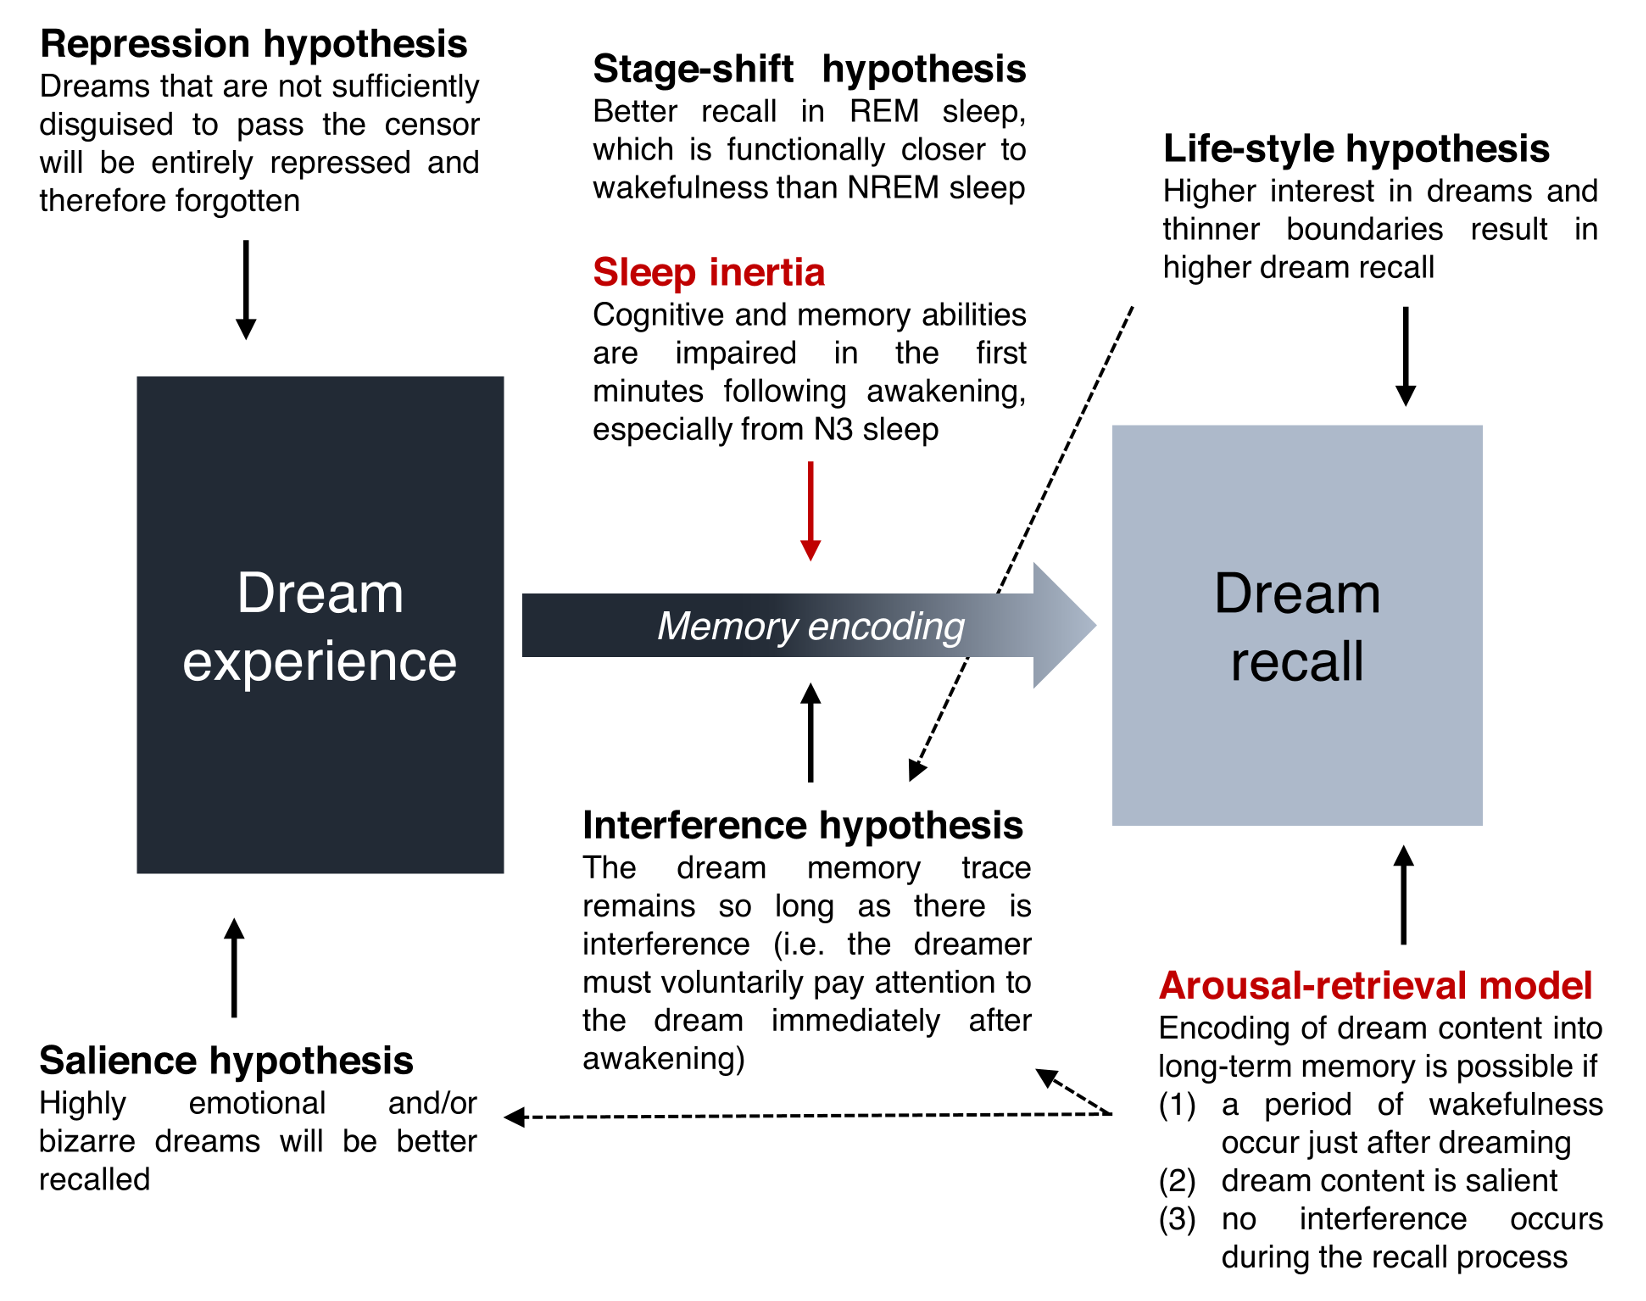
\includegraphics[width=\textwidth]{Fig/Intro/Intro_DRF_model/Intro_DRF_model.png}
	\caption[Dream recall theories]{\textbf{Dream recall theories.} The arousal-retrieval model provides so far the most comprehensive theory on dream recall and is firmly grounded in empirical evidence. At its simplest, it states that a short period of wakefulness must occur just after dreaming (arousal) in order to transfer the dream content from short to long term memory, which is otherwise impossible during sleep. In addition, it postulates that the dream content must be salient (Salience hypothesis, e.g. highly emotional, vivid and/or bizarre) and that the dreamer must voluntarily pay attention to the dream content (Interference hypothesis). Notably, it is very probable that the individuals with the greatest interest in dreams (Life-style hypothesis) are also the ones which focus the more on their dreams immediately after awakening, thus reducing encoding interferences. This would provide a link between the Life-style hypothesis and the arousal-retrieval model. Finally, sleep inertia could be a important explanatory factor with regards to DRF. It is possible that low dream recallers experience more acute sleep inertia upon awakening, whatever the sleep stage before awakening. More impaired memory and cognitive abilities upon awakening would in turn prevent the encoding of dreams to long term-memory. However, this hypothesis remains to be tested empirically.}
	\label{fig:intro:dream-recall-models}
\end{figure}

\cleardoublepage

\chapter{Dream content}
\label{sec:dream-content}

\cleanchapterquote{Prétendre donner les rêves comme de simples jeux de la pensée, de simples images de l’imagination, c’est témoigner d’un manque de réflexion ou de loyauté ; car de toute évidence ils en diffèrent spécifiquement. Les images de l’imagination sont faibles, languissantes, incomplètes, partielles et si fugitives qu’on peut à peine fixer dans sa mémoire pendant quelques secondes les traits d’un absent, et que même le jeu le plus vif de l’imagination ne peut nullement entrer en comparaison avec la réalité palpable que le rêve met sous nos yeux.}{Schopenhauer}{Parerga und Paralipomena, 1851}

\section{Basic principles of dream content analysis}
\label{sec:dream-content:method}

Empirical investigation on dreaming started in the nineteenth century when amateur researchers started to quantify aspects of their dream content. One notable example is the pioneering paper of Mary Calkins \citeyearpar{calkins_statistics_1893}, entitled \q{Statistics of dreams}, in which she reported, inter alia, statistics concerning dream length and vividness, dream characters and dream- and waking-life associations. Since then, a considerable numbers of scales and rating systems for dream content analysis have been developed \citep{schredl_dream_2010}. Most of them are based on automatic analysis of the lexical content of dream reports, a method which has the advantages of minimizing the experimenter bias and being replicable by other research groups. Perhaps the most famous is the Hall \& Van de Castle system, which have provided a global profile of dream content dimensions in young adult \citep{hall_content_1966}. It remains today the major reference since it has proven stable over at least one generation \citep{hall_dreams_1982}.

\section{Quantitative results}
\label{sec:dream-content:quant}

Results from several decades of dream content studies \citep{hall_content_1966, schwartz_exploration_1999, schredl_characteristics_2010} indicate that: dreams tend to be negative on many dimensions and aggressions are more frequent than friendly interactions, visual imagery occurs more frequently in dreams than imagery of other senses (audition, olfaction, touch, and taste); the dream drama is mostly lived by the dreamer from a first-person perspective; some elements of real-life events previously experienced by the dreamer often contribute to the scene of the dream; most often, the dream sequence is not within the dreamer’s voluntary control (i.e., the dreamer may be convinced during the dream that the dream’s story is really happening); temporal and spatial incoherencies can occur in the dream story; the dream report is often full of people interacting with each other (e.g., discussions, fights, pursuit, sexuality); and finally, the dream report often contains strong emotions.
Gender differences in dream content have been consistently reported. For example, men report more often physical aggression and sex than women \citep{nielsen_typical_2003, schredl_typical_2004}.
Finally, many aspects of the subject’s daily life influence dream content (reviewed in \citealp{ruby_experimental_2011}), including news event, musical practice, current concerns and religious beliefs, chronic pain, mood or living in a violent environment.

\section{The sources of dream content}
\label{sec:dream-content:sources}

Based on these experimental findings, \citet{de_koninck_sleep_2012} has reviewed in his book entitled \q{Sleep, dreams and dreaming} the sources that mediate dream construction, as well as their relative contribution to the dream content. He proposed that the different sources of dreams are best represented in a pyramidal manner, from low, more biological levels, predominant in shaping the dream content, to higher, more cognitive levels, that carry much less influence to the dream content (Figure \ref{fig:intro:koninck}).

\begin{figure}[htb]
	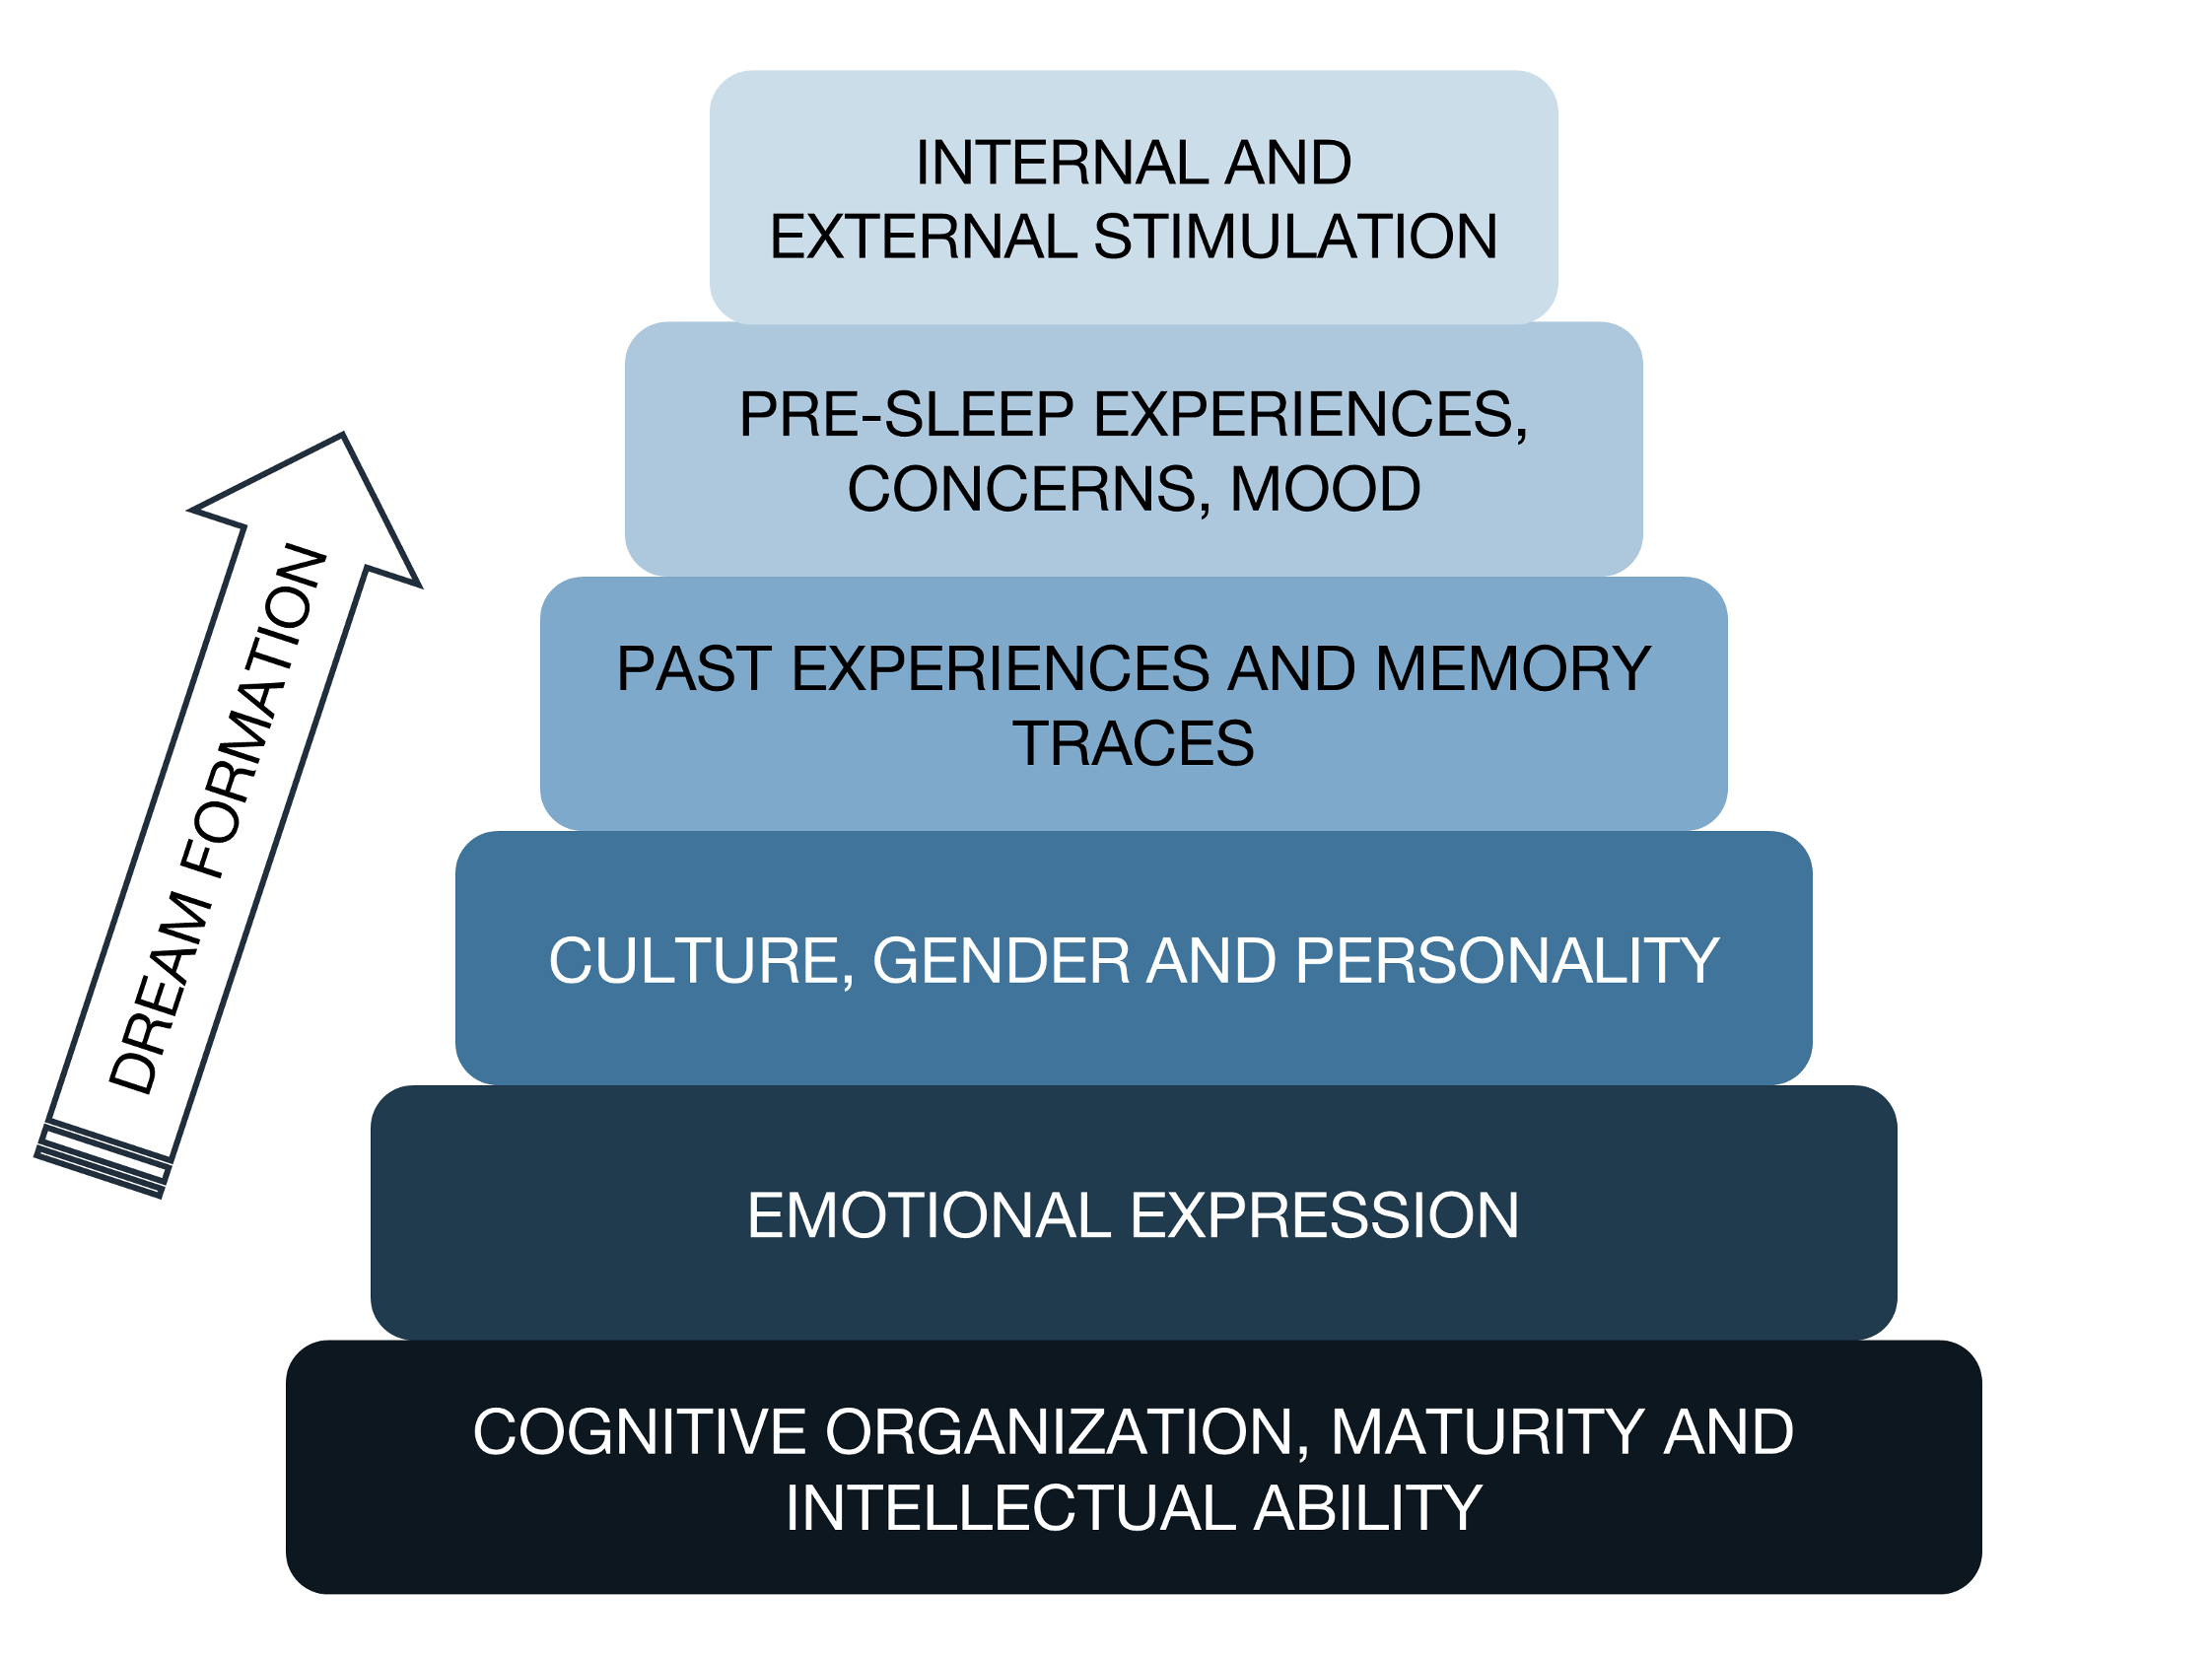
\includegraphics[width=\textwidth]{Fig/Intro/Intro_Pyramid_dream_construction/Intro_pyramid_dream.png}
	\caption[Layers in the construction of dreams]{Layers in the construction of dreams \citep{de_koninck_sleep_2012}. The various factors in the elaboration of dreaming are illustrated as a pyramid suggesting their order and importance.}
	\label{fig:intro:koninck}
\end{figure}

\subsection{The memory sources of dream content}
\label{sec:dream-content:sources:memory}

As we mentioned earlier, there is ample evidence that waking experience finds its way into dreams. However, the characteristics and time course of the waking memory sources integrated into dreams are still unclear. For instance, it is now clear that dream content very rarely replays an episodic memory as it is remembered \citep{fosse_dreaming_2003, nielsen_what_2005}, although it is often related to some elements of the waking life of the dreamer \citep{schredl_characteristics_2010, blagrove_trait_2010, ruby_experimental_2011}. This observation has led to the so-called \q{continuity hypothesis of dreaming} which simply states that dreams reflect waking life experiences \citep{schredl_continuity_2003}.

Several factors have been positively associated with the likelihood of a waking life experience to be incorporated into dreams \citep{schredl_characteristics_2010}. These factors are reviewed in the following lines. First, there seems to be a linear decrease in temporal references identified in dreams, with recent experiences being more incorporated into dreams than older ones \citep{botman_dream_1990, strauch_dem_2004, grenier_temporal_2005}. This finding supports the notion of continuity between waking and dreaming memory processes. Furthermore, several studies \citep{botman_dream_1990, nielsen_day-residue_1992, marquardt_empirical_1996} have confirmed that a significant proportion of dreams contain elements that refer to experiences of the preceding day, a phenomenon known as day-residues and mentioned by Freud who considered them as \q{a necessary ingredient in dream formation} \citep{freud_interpretation_1900}. Another interesting finding is that contrary to what would be expected according to memory decay with time, some studies reported an overrepresentation in dreams of waking experiences that happened approximately one week before the dream \citep{nielsen_day-residue_1992, marquardt_empirical_1996}, however this effect was found only for REM dreams and not N2 or N3 dreams \citep{blagrove_assessing_2011, van_rijn_dream-lag_2015}. Second, there is a preferential incorporation of emotional waking-life experiences into dreams \citep{malinowski_evidence_2014, schredl_factors_2006}. Interestingly, emotional intensity, but not emotional tone seems to affect the incorporation into subsequent dreams. Third, all waking life activities are not represented in the same proportion in dreams \citep{hartmann_we_1996, schredl_continuity_2000}. Focused thinking activity (such as using a computer, reading) are rarely reported in dreams, an effect that may be explained by the generally low emotional intensity of these types of activities. Fourth, the magnitude of the continuity between waking and dreaming is related to some extent to the personality traits of the dreamer \citep{schredl_dreaming_1996}. Finally, chronobiological factors, such as sleep cycles and time of the night, influence dream content. For example, dream reports from the first part of the night comprise more elements of the previous day than dream reports from the second part of the night \citep{roffwarg_effects_1978}.

\cleardoublepage

\chapter{Dream function}
\label{sec:dream-function}

\cleanchapterquote{J’ai rêvé tant et plus, mais je n’y entends note}{François Rabelais}{Pantagruel, 1532}

\section{Historical perspective}
\label{sec:dream-func:history}

\subsection{Ancient and classical history}
\label{sec:dream-func:history:ancient}

Since the dawn of times, humans have tried to assign meaning to their dreams. In many ancient civilizations, dreams were considered as omens or messages from deities, and needed therefore to be correctly interpreted. Numerous examples of dreams sent by Gods can be found in Mesopotamian, Egyptian and Greek mythological narratives, as well as in the sacred books of the three main monotheistic religions (see \citealp{de_koninck_sleep_2012}). Greek philosophers, however were the first to consider dreaming as a natural phenomenon. They provided different explanations of the nature and meaning of dreams, some of which are well in tune with modern dream research. For example, anticipating the notion of continuity between waking and dreaming, Cicero and Herodotus believed that dreams are produced by thoughts, concerns and conversations a dreamer had during the preceding days. Plato on the contrary viewed dreams as the expression of hidden desires and intolerable behaviors, an idea consistent with Freud’s repression hypothesis. Finally, Aristotle thought that dreams were caused by external and internal bodily sensations, an idea consistent with Hobson’s stochastic theory of dream generation.

\subsection{The royal road to the unconscious}
\label{sec:dream-func:history:psychanalysis}

The father of psychanalysis viewed dreams as the \q{royal road to the unconscious} \citep{freud_interpretation_1900}. He defined the unconscious as a part of our mind made up of thoughts, desires, emotions, and knowledge that we are unaware of, but that nevertheless profoundly influence and guide our behaviors. Freud believed that the ego’s defenses are lowered during dreaming, which allows the unconscious mind and the repressed material (i.e. hidden desires) it conveys to come through awareness, albeit in a distorted form. For him, the dream is formed of the manifest content (i.e. the dream as the dreamer recalls it), which is often based on mundane and insignificant day-residues, and the latent content (i.e. symbolic meaning of the dream). The latent content of the dream can be translated into manifest content (a process referred to as dream work) in order to unravel the underlying wish and hidden desires present within the dream. Therefore, in Freud’s model, the dream need to be explicitly remembered and interpreted to possess an adaptive value. It is noteworthy that his hypothesis \q{has rarely been considered by neuroscientists who often consider Freud’s work and theory unscientific} \citep{ruby_experimental_2011}.

\subsection{Psychological individualism}
\label{sec:dream-func:history:jouvet}

Michel Jouvet, one of the pioneers of sleep research, co-discoverer of REM sleep, was also greatly interested in dreams. He kept a dream diary for years, which he used to describe several quantitative measures on dream content. For instance, he was one of the first to report high residue frequencies in dreams approximatively one week days the waking experience (i.e. the dream-lag effect; \citealp{jouvet_memoire_1979}). Regarding the function of dreams, which he equated at the time to the function of REM sleep, he proposed that it is a kind of iterative neurological programming which aims at preserving the expression of the genetic program that codes for psychological characteristics. According to him, this process would ensure the stability of personality across time \citep{jouvet_sommeil_1991}.

\section{Modern theories}
\label{sec:dream-func:modern}

\subsection{An epiphenomenom of REM sleep}
\label{sec:dream-func:modern:nofunc}

Based on the neurophysiological properties of REM sleep, which he equated with dreaming, Alan Hobson proposed that dreaming is an epiphenomenon of REM sleep \citep{hobson_dream_1998}. According to him, the dream imagery is the result of cortical centers trying to create meaning from brainstem-driven signals generated during REM sleep (the so-called activation-synthesis model). In this theory, the dream content is therefore stochastic and is very unlikely to represent an adaptive advantage. It should be noted, however, as noticed by \citet{windt_dreaming:_2015}, that \q{Hobson does not deny that dreams can have meaning and can reflect the personality and concerns of the dreamer. He just thinks that their meaning is transparent and immediately obvious to the dreamer, rather than requiring an elaborate process of interpretation.}

\subsection{Threat / Social simulation theory}
\label{sec:dream-func:modern:revonsuo}

\citet{revonsuo_reinterpretation_2000} proposed that dreaming is a virtual reality in which the dreamer can simulate threatening events and therefore be better prepared to face upcoming dangers in waking life (the so-called threat simulation theory, TST). According to him, \q{dream consciousness is essentially an ancient biological defense mechanism, evolutionarily selected for its capacity to repeatedly simulate threatening events} \citep{valli_threat_2005}. As such, dream content is more consistent with the original evolutionary environment of the human species (e.g. high level of violence and intergroup aggression between males) rather than the present one, and this could for example explain that the most frequent type of social interaction found in dreams, especially in males, is aggression \citep{hall_content_1966}. \citet{valli_threat_2005} further tested this hypothesis by analyzing the content of dream reports from severely traumatized and non-traumatized children. As expected by the theory, the dreams of severely traumatized children reported included a higher number of threatening events, which were also more severe in nature than the threats of non-traumatized children.
The same team has recently proposed that, more than a simulation of threats, dreaming is a platform for simulating social perception and interactions (the so-called social simulation theory, SST; \citealp{revonsuo_avatars_2015}), which are, from an evolutionary standpoint, as relevant as threats (it is now well accepted that the social environment has afflicted strong selection pressures on human cognition).

\subsection{Memory consolidation}
\label{sec:dream-func:modern:memory}

There is converging evidences from both animal and human research that sleep optimizes the consolidation of newly acquired information in memory \citep{rasch_odor_2007, diekelmann_memory_2010}. Based on this, a current hypothesis in dream research is that dreaming per se is related to sleep-dependent memory consolidation (review in \citealp{schredl_is_2017}).
This proposal was tested in \citet{wamsley_dreaming_2010} in a study where 50 subjects were trained on a  virtual navigation task before taking a 45 min nap. Remarkably, subjects who dreamed about the task had better post-nap performances than subjects who did not dream. However, as only 4 out of 50 subjects actually dreamed about the task (among which two reports just included hearing the music presented during the training session), the statistical power of this study is very low and it would seem premature to draw conclusions from this single finding. The same year, \citet{schredl_is_2010} investigated whether dream characteristics are related to the over-night improvement of a mirror tracing task (i.e. the participants must trace different figures they only saw in a mirror). They were unable to find an effect of direct incorporations of the mirror tracing task into the dream on over-night improvement. It should be noted however that, again, the rate of direct incorporation of the task was very low, which consequently results in a low statistical power. Another methodological bias is that these studies focused only, and for obvious reason, on recalled dreams and thus omit a large fraction of non-recalled dreams. The role of the different sleep stages in the putative role of dreaming in memory consolidation needs to be further investigated. To sum up, these results are hitherto inconclusive on the role of dreaming in memory consolidation.

\subsection{Emotional regulation}
\label{sec:dream-func:modern:emotion}

Cartwright proposed that dreaming is involved in emotional regulation \citep{cartwright_role_1998, cartwright_role_1998-1}. She reached this conclusion after observing that, in healthy subjects, the depression level before sleep was significantly with affect in the first REM report. On the same study, she also observed that low scorers on the depression scale displayed a flat distribution of positive and negative affect in dreams, whereas those with a depressed mood before sleep showed a pattern of decreasing negative and increasing positive affect in dreams reported from successive REM periods. Secondly, she observed that among individuals who were depressed following a divorce, those who reported more negative dreams early in the night and fewer at late-night were more likely to be in remission one year later, compared to subjects in which this pattern was inverted. From these two works, she proposed that dreaming may actively moderate mood overnight in healthy individuals, with the decreasing rate of negative dreams across the night reflecting a within-sleep emotional regulation process.
Linking emotional regulation and memory consolidation processes, \citet{perogamvros_roles_2012} recently proposed the Reward Activation Model according to which emotionally relevant experiences (including threat-related information) have a higher probability of being activated during sleep and have a preferential access to sleep-related memory consolidation processes. According to them, one of the main functions of dreaming is \q{to expose the sleeper to rewarding or aversive stimuli, in order to maintain and improve offline memory consolidation processes and performance in real life situations, while also contributing to emotion regulation processes} \citep{meerlo_sleep_2013}.

\subsection{Summary}
\label{sec:dream-func:modern:summary}

Despite several decades of scientific research on dream content, there is still no consensus on whether dreaming serves a function or not. To move forward on this issue, researchers should try to experimentally test, if possible, the predictions beyond all those hypothesis.
On another note, several fundamental questions arise from these works, as noticed by \citet{de_koninck_sleep_2012}. If dreams do have a function, do they need to reach consciousness and be remembered in order to be functional? Or do they need to be worked, or interpreted as believed by Freud and in many ancient civilizations?

\cleardoublepage

\chapter{Hypothesis and objectives}
\label{sec:problematic}

\cleanchapterquote{Le fait de rêver est sans doute une des données, plus nombreuses qu'on ne le pense, qui, mieux encore que le soleil ou la pluie, placent les hommes de tout climat, de toute époque et de toute condition devant des problèmes identiques.\endnote{Free translation to English: \q{Dreaming is undoubtedly one of the phenomenon, which, better than the sun or the rain, places men of any climate, of any time and any condition in front of identical problems} ---Roger Caillois. L'incertitude qui vient du rêve. 1956}}{Roger Caillois}{L'incertitude qui vient du rêve. 1956}

\section{Unresolved issues}
\label{sec:problematic:unresolved}

From this review of the scientific literature on dreaming, it appears that many questions on the nature, function, and neurophysiological correlates of dreaming remain open, some of which are reported below.

\textbf{Phenomenology of dreaming}
\begin{my_list_item}
    \item Do we dream during the whole night? If not, when do we dream during the night and for how long?
	\item Which factors influence the (dis-)continuity between waking and dreaming?
	% \item Why is there a preferential incorporation of certain waking experiences into dreams?
	\item What are the neurophysiological correlates of dream content? And can we explain the phenomenological content of dream content based on these correlates ?
	\item To what extent lucid dreaming resemble or differ from non-lucid dreaming?
	\item To what extent dreaming resemble or differ from other forms of spontaneous thoughts such as mind-wandering and daydreaming?
\end{my_list_item}

\textbf{Dream recall}
\begin{my_list_item}
	\item Why are there such intra- and inter-individual differences in dream recall frequency?
	\item What are the neurophysiological correlates of dream recall?
    \item Why more dream reports follow awakening from REM sleep than from NREM sleep? Does that mean that the actual \emph{production} of dreams is higher during REM sleep than NREM sleep, or rather than the \emph{recall} of dreams is better following REM sleep?
	\item More broadly, does failure to recall dream upon awakening mean that the sleeper was not dreaming before awakening? Or does this reflect a failure to encode dream content into memory, for example caused by sleep inertia or interference mechanisms?
\end{my_list_item}

\textbf{Function of dreaming}
\begin{my_list_item}
	\item Do dreaming serves an adaptive function \emph{per se}? If so, do they need to reach consciousness and be remembered in order to be functional? Or do they need to be worked, or interpreted as believed by many?
\end{my_list_item}

The present thesis aims at contributing to the ongoing effort to solve these questions, by addressing, in parallel and with different paradigms, several aspects of dreaming. First, we investigated the mechanisms of dream recall by comparing the cerebral and behavioral functioning of high and low dream recallers (HR and LR, respectively). In Study 1 (section \ref{sec:problematic:arousals}), we used EEG recordings to compare the sleep macro- and micro-structure of HR and LR, as well as their brain responses to stimuli during sleep. In Study 2 (section \ref{sec:problematic:inertia}), we compared the cognitive performances and brain functional connectivity of HR and LR during sleep inertia using an EEG-fMRI paradigm. In addition with studying the mechanisms of dream recall (sub-study 1), this study was one of the very first to measure, in healthy subject, the brain functional connectivity alterations during sleep inertia (sub-study 2). In Study 3 (section \ref{sec:problematic:dmn-crea}), we further analyzed the data of this EEG-fMRI study to specifically compare the global default mode network functional connectivity in HR and LR, regardless of the effect of sleep inertia. At the same time, we measured, and compared between HR and LR, several cognitive and personality variables. In Study 4 (section \ref{sec:problematic:survey}), we took advantage of the considerable number of responses obtained in the online recruitment survey of this EEG-fMRI study to collect epidemiological data on dream and sleep habits of a large sample of French college students. In Study 5 (section \ref{sec:problematic:wle}), we used dream questionnaires to improve our understanding of the filter that dreaming applies to the waking life memories, and at the same time try to decipher the possible functions of dreaming. Finally, in Study 6 (section \ref{sec:problematic:software}), we leveraged our expertise in sleep analysis to develop a free and open-source software dedicated to the reading, scoring and analysis of sleep data.

\section{Study 1. DRF and intra-sleep awakening: brain mechanisms and functional properties}
\label{sec:problematic:arousals}

We have seen in section \ref{sec:dream-recall:param} that HR tend to have longer awakenings than LR during sleep (2 vs 1 min on average), and consequently a longer duration of intra-sleep wakefulness (30 vs 15 min on average in a full night of polysomnographic-recorded sleep), without any other differences in the duration and proportion of sleep stages \citep{eichenlaub_brain_2014}. These findings support the arousal-retrieval model which states that nocturnal awakenings are necessary to encode dreams into long-term memory. However, if awakenings are crucial for dream recall as these findings seems to suggest, one may ask if there is a minimum duration of awakenings to allow for the successful encoding of dreams into long-term memory, and if so, if this duration varies depending on the pre-awakening sleep stage. This issue was not directly addressed by \citet{koulack_dream_1976}, who merely stated that arousal have to be of \q{sufficient duration to permit consolidation of the dream experience in a form that is accessible in the waking state}.

Consequently, we decided to experimentally test this issue by re-analyzing the data of \citet{eichenlaub_brain_2014} (see section \ref{sec:dream-recall:param:neuro}) in order to score arousals. Arousals correspond to short and physiological awakenings lasting typically between 3 and 15 seconds, and scored independently of the sleep stages \citep{american_sleep_disorders_association_eeg_1992, de_gennaro_eeg_2001, bonnet_scoring_2007, bonnet_eeg_2007}. In addition with the scoring of arousals, we performed a close comparison of sleep microstructure of HR and LR, in order to extent our knowledge of the influence of sleep parameters on DRF. This analysis included spindles, K-complexes, rapid eye movements and muscle twitches, which were scored either visually or automatically using dedicated algorithms. We also re-examined the data to see whether the longer awakening duration found in HR was limited to a specific sleep stages (e.g. longer nocturnal awakenings following periods of REM sleep), or was present in all sleep stages.

Second, we took the opportunity of the arousals scoring to address another issue, which is related to the finding of differential brain reactivity to auditory stimuli in high and low dream recallers (see section \ref{sec:dream-recall:param:neuro}). As a reminder, \citet{eichenlaub_brain_2014} found that the amplitude of the attention-orienting brain response (P3a) to first names was higher in HR than in LR during both sleep and wakefulness (Fig \ref{fig:intro:jbe-summary}A). These findings, along with the longer intra-sleep wakefulness in high recallers, suggest that there might be a causal link between neurophysiological responses to auditory stimuli and intra-sleep wakefulness during sleep. For instance, the amplitude of brain responses to auditory stimuli could be predictive of subsequent awakening or arousal reactions. Consequently, HR, who have larger brain responses to auditory stimuli, would have in turn more or longer awakenings during sleep and therefore more opportunities to encode their dreams into long term memory. One way to test this hypothesis would be to show that the amplitude of brain responses to auditory stimuli inducing an awakening or an arousal reaction is significantly higher than the amplitude of brain responses to stimuli that does not induce such reactions. Remarkably, this effect has already been reported for painful stimuli by \citet{bastuji_laser_2008}, who found that \q{a late positive component (450–650 ms) was recorded in both stage 2 and paradoxical sleep, the amplitude of which was significantly enhanced in trials that were followed by an arousal}. According to the authors, this brain response, which appeared functionally related to the P3 wave, might be associated to conscious perception and memory encoding. At the time of the original study, \citet{eichenlaub_brain_2014} were however not able to test this hypothesis given that they did not have the arousals scoring and that only too few auditory stimuli induced awakening reactions. The scoring of arousals, which are physiologically far more numerous than awakenings, made it possible to compare the auditory evoked potentials to arousing and non arousing stimuli.

Our predictions were the following ones. First, we expected no differences in the sleep microstructure of HR and LR, including the number and density of arousals, rapid-eye movements, spindles and K-complexes. Our hypothesis was that intra-sleep awakening, and not sleep microstructure, is the critical factor to explain variability in DRF. In line with this, we predicted that the duration of intra-sleep awakenings should be higher, in HR as compared to LR, whatever the sleep stages prior to awakening is. Third, consistent with previously reported with painful stimuli, we expected that the amplitude of brain responses to arousing auditory stimuli will be significantly higher than the one of non-arousing stimuli, i.e. that larger brain responses predict subsequent awakening or arousal reactions. If this is the case, this result would provide a strong argument in favor of a causal link between brain responses during sleep, nocturnal awakenings, and dream recall frequency.

\section{Study 2. The awakening brain: sleep inertia and its relationship to DRF}
\label{sec:problematic:inertia}

\subsection{Sub-study 1: Sleep inertia in high and low dream recallers}
\label{sec:problematic:inertia:drf}

To reiterate an earlier quotation (section \ref{sec:dream-recall:theories:inertia}), \q{quite possibly, brain functioning underlying the reporting and non-reporting of dreams does not exist within the pre-sleeping period at all, but within the period just after awakening, when cognitive resources are in demand to recall and/or consolidate events which have just occurred within the previous sleeping period} \citep{conduit_poor_2004}. This is particularly interesting given that the \q{period just after awakening} is characterized by reduced vigilance, sleepiness and impaired performances, a state often referred to as sleep inertia. Although its duration is not consensual and varies depending on the outcome measure used, it is generally admitted that most of the behavioral effects of sleep inertia dissipate progressively in the first 30 minutes post awakening. Severity of sleep inertia has been positively associated to several factors such as prior sleep deprivation, awakening near the circadian trough of body temperature and awakening in N3 sleep (see \citealp{tassi_sleep_2000} for a review).

With regards to dream recall, the impaired cognitive functioning in the minutes following awakening could be indeed detrimental to recall and/or encoding of dreams \citep{conduit_poor_2004}. As pointed out by \citet{schredl_factors_2003}, it would be in consequence \q{promising to correlate inter-individual differences regarding the sleep inertia with DRF}. One could expect that low dream recallers would suffer from more acute sleep inertia upon awakening and that stronger impairment of cognitive functioning would prevent the short term memory of dreams from surviving the sleep-wake transition. By contrast, high dream recallers would suffer from less sleep inertia and would consequently have less difficulty to recall and/or encode dreams.

Very little attention has hitherto been devoted to this hypothesis, and no experimental studies have either supported or refuted it. In order to fill this gap, we designed a combined EEG-fMRI study to investigate sleep inertia in high and low dream recallers in the minutes following awakening from a 45 minutes mid-afternoon nap (see Fig \ref{fig:intro:problematics-fmri-paradigm}). Resting-state scans were acquired before the nap, 5 min and 25 min after awakening to investigate the brain functional connectivity during sleep inertia in the two groups, and each scan was associated with a mental calculation task to measure the cognitive impairments associated with sleep inertia. We predicted that high dream recallers would show (1) more frequent dream recall upon awakening (2) a higher functional connectivity within the default mode network (see section \ref{sec:dream-research:attempts:dmn} and \ref{sec:dream-recall:param:neuro}) (3) less cognitive performance impairments, suggesting a faster recovery from sleep of regions involved in executive and memory processes. In other words, we hypothesized that the brain functional organization during sleep inertia would differ between high and low dream recallers and would reflect between group differences in dream recall.

\begin{figure}[!htbp]
	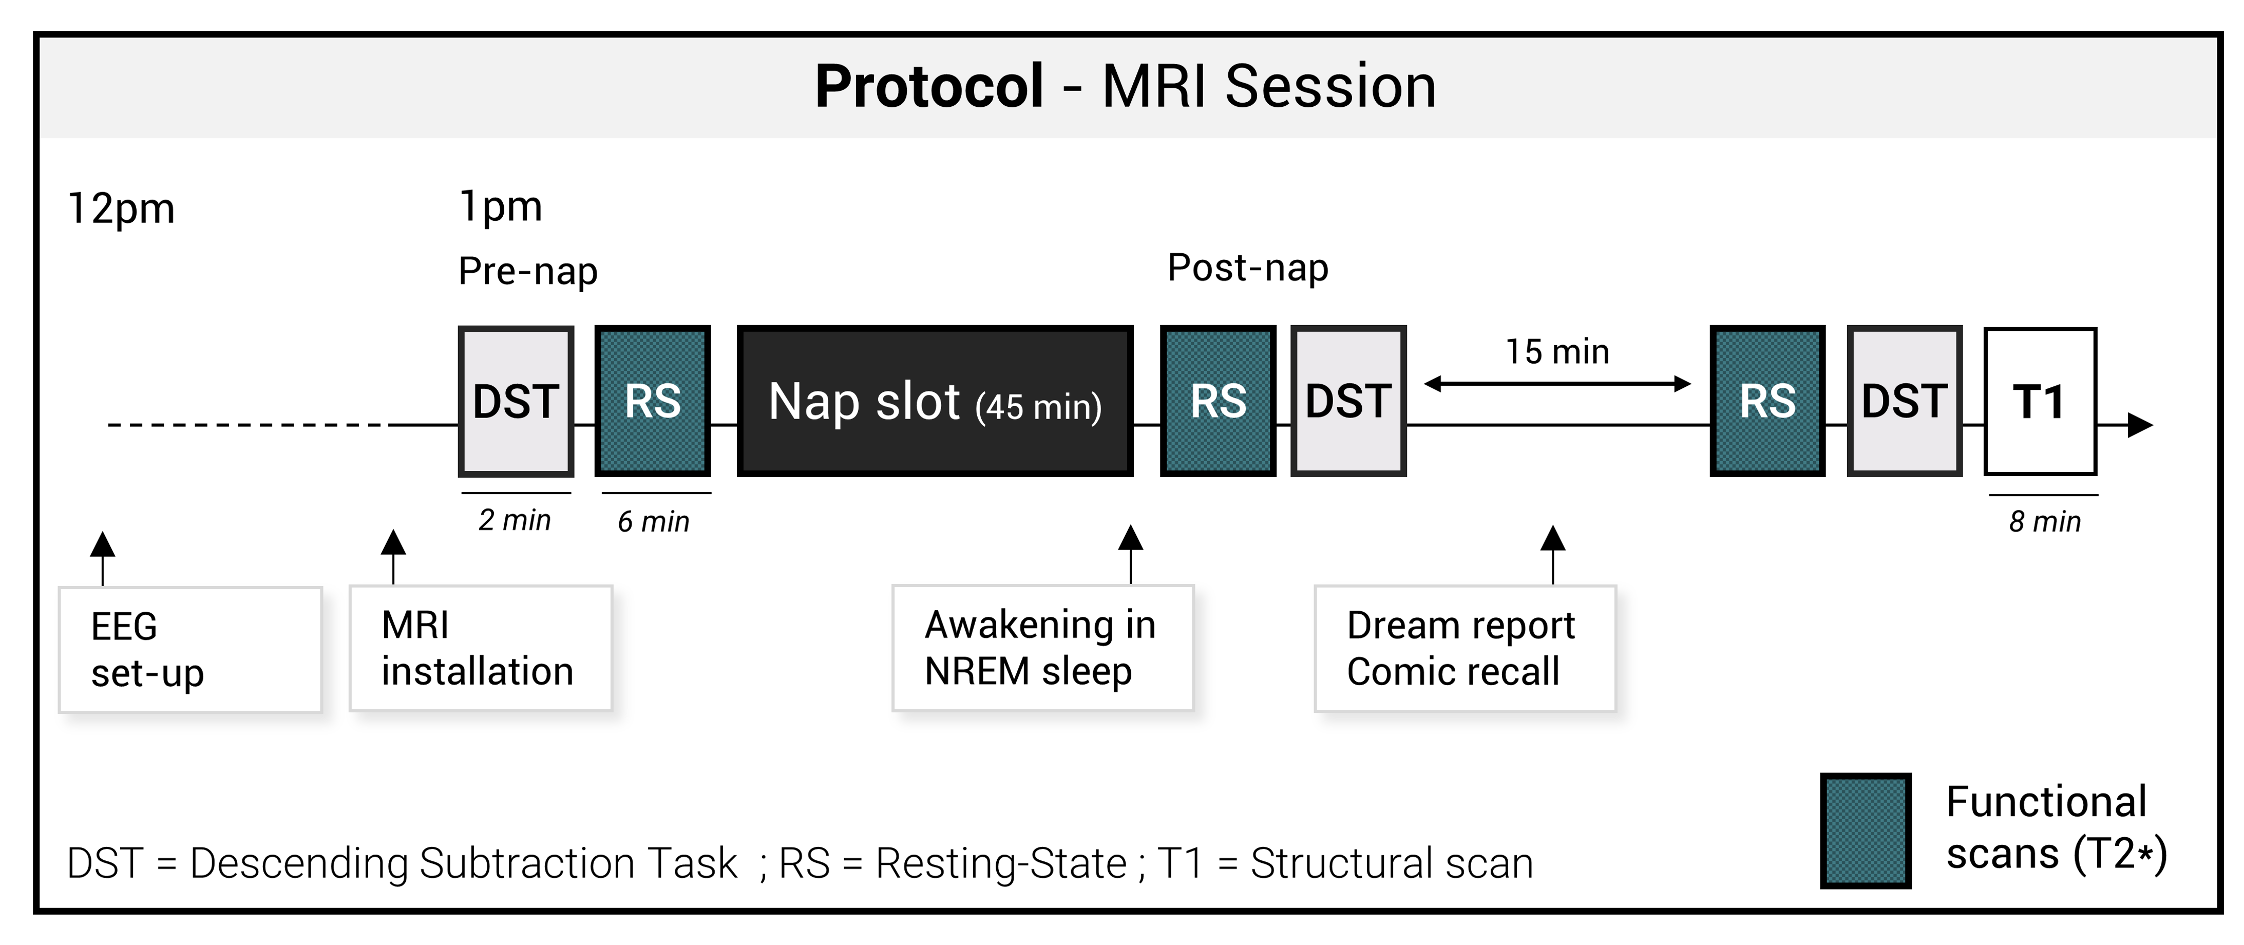
\includegraphics[width=\textwidth]{Fig/Intro/Intro_paradigm_fMRI/Intro_paradigm_fMRI.png}
	\caption[Experimental design of the fMRI study]{\textbf{Experimental design of the sleep inertia fMRI study}. \\
    \emph{Participants}. Participants were selected if they reported and subsequently confirmed during a phone interview having a high or low DRF (DRF superior to 5 dream recalls per week and inferior to 2 dream recalls per month respectively) and having no sleep disturbances. \\
    \emph{Evening and night}. Participants arrived in the sleep unit of the hospital Le Vinatier (Lyon, France) at 8 pm on the evening prior to the experimental day. From 8 pm to 10 pm, they underwent several personality and cognitive tests administered by R.V. They were then instructed to stay awake until 5 am, at which point they were allowed to sleep for 3 hours until 8 am in a bed in the sleep unit. \\
    \emph{Day}. After lunch, participants were conducted to the neuroimaging center (CERMEP). During the first half hour, experimenters installed on the participant’s head a MRI compatible EEG cap. Participants were then installed in the MRI scanner. They read a 5 min comic during the calibration of the eye-tracking camera, and then performed a mental calculation task (descending subtraction task, DST) for 2 minutes. The first resting-state scan was then acquired, with the instructions to remain awake and look at a central fixation cross on the screen. At the end of the scan, participants were informed that they could sleep during the next 45 min. During the nap, the experimenter used the EEG recordings to visually monitor, in real-time, the sleep stages. At the end of the nap slot, participants were awakened, if they were sleeping, by calling their first name and the 2nd resting state scan was acquired. At the end of the scan, the 2nd DST was performed. During the following 10 minutes, subjects were asked about their dream(s) and the comic they had read earlier. Then the 3rd resting state scan and DST were performed (about 25 min after awakening). Finally, an 8-min T1 anatomical scan was acquired.}
	\label{fig:intro:problematics-fmri-paradigm}
\end{figure}

\subsection{Sub-study 2: Brain networks dynamics during sleep inertia}
\label{sec:problematic:inertia:overview}

In addition with comparing the differential brain functional organization of high and low dream recallers during sleep inertia, this study offers the possibility to investigate thoroughly - by pooling the two groups - the brain networks changes across the sleep inertia period. Indeed, while the behavioral aspects of sleep inertia are well documented, only a limited amount of studies investigated its cerebral correlates until now. Our paradigm offers an unique opportunity to study the brain and cognitive alterations during sleep inertia. For instance, one can observe the alterations in functional connectivity that are specific to sleep inertia by contrasting the 5 min post-awakening fMRI scan (RS2, see Fig \ref{fig:intro:problematics-fmri-paradigm}) to the pre-sleep fMRI scan (RS1). Similarly, the evolution of the cerebral alterations of sleep inertia can be evaluated by contrasting the 25 min post-awakening fMRI scan (RS3) to the 5 min post-awakening scan (RS2). In sum, by assessing simultaneously the brain and behavioral changes associated with sleep inertia, our paradigm provides an ideal starting point to study, as wished by \citet{trotti_waking_2016} in her recent review, \q{the which and how functional brain networks are altered in the minutes following awakening}. It should also be noted that participants were partially sleep deprived on the night before, and awakened from a 45 minutes mid-afternoon nap if possible in N3 sleep. Both sleep deprivation and awakening in N3 sleep have been associated with increased sleep inertia \citep{tassi_sleep_2000}. Therefore, in addition with being ecological (short nights compensated by a daytime nap being common in young adults \citep{faraut_napping:_2016}, this paradigm will allow us to study sleep inertia in its most intensified form.

% Using EEG, some studies have found a persistence of slow wave activity in the minutes following awakening, specifically in posterior areas, a phenomenon which has been suggested to represent the electro-physiological signature of sleep inertia \citep{ogilvie_falling_1992, ferrara_electroencephalographic_2006, marzano_recalling_2011, gorgoni_eeg_2015}. Using PET, \citet{balkin_process_2002} reported that the brain areas whose regional cerebral blood flow (rCBF) was increasing between 5 to 20 min post awakening were primarily anterior heteromodal areas (e.g. lateral prefrontal cortices, and anterior insula). They also reported shifts in the relative levels of rCBF between pairs of brain regions (orbitofrontal cortex and ventromedial caudate nucleus, dorsolateral prefrontal cortex and mesencephalic reticular formation) between 5 and 20 min post awakening, leading them to propose that recovery from sleep inertia could hinge on a resumption of normal levels of both rCBF and functional connectivity between brain areas. The latter hypothesis has been tested in two recent resting-state functional magnetic resonance imaging (fMRI) studies which investigated the variations in brain connectivity between pre-sleep wakefulness, nocturnal sleep (without previous sleep deprivation) and post-sleep wakefulness \citep{wu_variations_2012, tsai_local_2014}. Using paired comparisons between pre- and post-sleep wakefulness, they found a decreased connectivity within the sensory-motor network at awakening but no alterations in the default mode network. This altered connectivity within the sensory-motor network is coherent with the poor motor performances observed at awakening but does not explain the impairments observed in other domains (e.g. cognitive tasks such as mental calculation, \citealp{tassi_sleep_2000, trotti_waking_2016}). Yet, some modifications of the default mode network connectivity could be expected at awakening since several neuroimaging studies showed consistent alterations of the default mode network connectivity during sleep, fatigue and/or falling asleep (see \citealp{picchioni_sleep_2013} for a review).

\section{Study 3. DRF, cognitive abilities, and default network functional connectivity}
\label{sec:problematic:dmn-crea}

As we have seen earlier, there is ample evidence that DRF is positively correlated with psychological factors such as creativity or some personality traits (e.g. openness to experience, see section \ref{sec:dream-recall:param:psych} and \ref{sec:dream-recall:param:psych}). On the other hand, recent findings indicate that DRF is also positively associated with distinct neurophysiological traits during both sleep and wakefulness, such as a higher regional cerebral blood flow within core regions of the default mode network. These two observations are remarkably consistent with the emerging view that dreaming and creative-thinking pertain to the same family of spontaneous mental processes, which could be underpinned by a strong recruitment of the default mode network (DMN, \citealp{christoff_mind-wandering_2016}, see section \ref{sec:dream-research:attempts:dmn}) To better delineate the relationship between DRF and the DMN, we re-analyzed the fMRI data of Study 2 to compare, between HR and LR, the functional connectivity of the default mode network, independently of sleep inertia. To this aim, we concatenated the three resting-state scans acquired for each subject, and subsequently compared the global DMN functional connectivity of HR and LR.

Furthermore, we analyzed in this study the numerous cognitive and personality tests that were administered between 8pm and 10pm, on the evening prior to the partial sleep deprivation. Examples of these include the Guildford's Alternate Uses Task \citep{guildford_alternate_1978}, which measures creativity, the Wechsler Memory Scale \citep{wechsler_mem-iii:_2001} to measure memory abilities, and the Big Five Inventory \citep{john_big_1999} which measures an individual on the big five personality dimensions. Regarding the results, we expected that HR would exhibit a higher DMN functional connectivity, specifically between the TPJ and MPFC (see section \ref{sec:dream-recall:param:neuro}), as well as higher scores of creativity and higher scores on certain personality dimensions such as openness to experience. In view of the literature, we did not expect HR to show higher memory abilities than LR.

\FloatBarrier

\section{Study 4. Sleep and dream habits in a sample of French students}
\label{sec:problematic:survey}

Epidemiological investigations in healthy subjects combining questions on both sleep and dreaming are relatively rare. Such measures are yet necessary to establish and keep up to date sleep and dream norms in the general population. Of particular interest is the college population, which is more at risk of suffering from sleep difficulties than the general population \citep{buboltz_sleep_2001, curcio_sleep_2006, forquer_sleep_2008, lund_sleep_2010}.

In order to recruit participants for our above-mentioned fMRI sleep study (section \ref{sec:problematic:inertia}), we have sent an announcement to several mailing lists of students from Lyon University. The announcement comprised a link to an online questionnaire about sleep and dream habits that participants had to fill out. The analysis of the responses provided up-to-date data on sleep and dream habits of a large sample of French college students, pertaining to different academic fields (i.e. humanities, science, medicine). Because our survey included relatively rare questions (e.g. frequency of recurrent and lucid dreams, sleepwalking, sleep-talking, sleep agitation), and thanks to a large sample of students including much more males than in previous studies (i.e. more than one third), we believe that this study will make a significant contribution to the limited number of previous epidemiological studies. Among our main points of interests were (1) to evaluate the sleep patterns of French college students (2) to find whether we could replicate previously reported gender differences in sleep and dream patterns (3) to find whether we could observe some inter academic fields differences.

\section{Study 5. The relationship between waking life and dream content}
\label{sec:problematic:wle}

As we mentioned earlier, there are numerous results showing that waking-life experience (WLE) finds its way into dreams (which led to the so-called continuity hypothesis, \citealp{schredl_continuity_2003}). However, the selection rule and time course of the WLE integration into dreams are still unclear. For instance, few studies have so far investigated the incorporation of WLE from the distant past as well as the incorporation of trivial, mundane, WLE. This is partly due to the classic method used in experimental studies so far, i.e. the content matching paradigm. It requires the participants to rate a posteriori (i.e. at the end of several days of experiment), similarities between a day diary and a dream diary completed for 14 days (e.g. \citealp{schredl_factors_2006, malinowski_evidence_2014}). Such a method has the advantage of controlling for retrospective availability of memories for elements when participants relate dream content to WLEs, but it may have the drawback of missing numerous mundane WLE that are not recorded in the day diary (typically insignificant day-residues), and at the same time overestimating the proportion of emotionally intense WLE. As a consequence, previous studies could not fully assess whether mundane WLEs and/or WLEs from the distant past were incorporated into dreams.

% This is the case for instance regarding the temporal distance between the WLE and its incorporation into dreams on one hand, and the emotional intensity of the WLE on the other hand. Indeed, it is generally admitted that there is a preferential incorporation of recent and emotional WLE into dreams \citep{botman_dream_1990, strauch_dem_2004, grenier_temporal_2005, schredl_factors_2006, malinowski_evidence_2014}. However, some characteristics of dream content do not fit with this modeling of the data. Firstly, some body injuries - be it congenital or acquired - such as amputation, paraplegia and deafness, are less incorporated into dream reports than this model would predict considering how highly emotional and central to the person’s life they are \citep{voss_waking_2011, saurat_walking_2011, bekrater-bodmann_post-amputation_2015}. Secondly, as noticed by \citet{freud_interpretation_1900} more than one century ago, dream content seems to integrate a non-negligible proportion of non-emotional and mundane day residues (i.e. WLEs from the day before the dream).

To address this problem, we designed a study which aimed at investigating in further details the characteristics of the WLEs incorporated into dreams, notably by assessing their remoteness on a life-time scale and by taking mundane WLEs into account. To do so, instead of asking dreamers to keep a day diary, we asked participants to report and characterize the WLEs related to their dreams immediately upon awakening. This strategy presents several advantages regarding previous methods. Firstly, any remembered WLE at any timescale can be considered. This method offers then the possibility of investigating the incorporation of WLEs across the whole life span, which has been rarely attempted until now \citep{grenier_temporal_2005, marquardt_empirical_1996}. Secondly, as the reported memory sources of a dream are dependent on the delay between the dream and the task to report memory sources, the sooner the task after the dream, the more chances we have to identify the true memory sources of the dream \citep{cavallero_dream_1987}. Thirdly, as the connections between elements of waking life and dream content are assessed when the memories of the preceding days are still fresh, this method enables the recall of trivial WLEs from at least the few days before the dream. Using this new approach, we were able to test whether emotional WLEs are still preferentially incorporated into dream reports when trivial WLEs are taken into account and to investigate the emotionality and significance of WLEs incorporated into dreams as a function of their remoteness.

We predicted that this methodology would enable us to observe that a large proportion of the WLEs incorporated into dreams are mundane. Regarding the temporal remoteness of the WLEs incorporated into dreams, we expected to find not only a large contribution of the day before the dream \citep{marquardt_empirical_1996} but also a significant contribution of remote WLEs \citep{verdone_temporal_1965, grenier_temporal_2005, llewellyn_such_2013}. Finally, given previous results showing a tendency for dreams to incorporate preferentially emotional WLEs \citep{schredl_factors_2006, malinowski_evidence_2014}, and the claim that day residues are predominantly mundane \citep{freud_interpretation_1900}, we predicted an interaction between remoteness and emotionality for WLEs incorporated into dreams. Specifically, we expected that day residues would be scored as less important and less emotionally intense than would be more remote WLEs incorporated into dreams.

\section{Study 6. An open-source software for sleep reading and analysis}
\label{sec:problematic:software}

During my PhD thesis, I have been working extensively on polysomnographic sleep recordings, notably to score sleep microstructural events (e.g. arousals, rapid eye movements; see section \ref{sec:problematic:arousals}) and sleep stages (see section \ref{sec:problematic:inertia}). While the detection of sleep microstructural events is usually done with automatic algorithms, the identification of sleep stages is traditionally done visually by an expert. For both visual sleep staging and automatic microstructural analysis, sleep researchers use either commercial or in-house softwares. In many cases, these softwares come with their own data and hypnogram file formats, and this heterogeneity can represent a substantial obstacle for sharing of algorithms and sleep data across laboratories.

% Some of the very few free and open-sources alternatives allowing scoring and to some extent analysis of sleep data are \fnurl{Phypno}{https://pypi.python.org/pypi/phypno} and \fnurl{SpiSOP}{http://www.spisop.org/}, yet they do not include graphical integration of automatic detection and are largely based on command-line options, which are hardly accessible for users with little or no programming knowledge.

% Traditionally, the scoring of sleep micro- and macro-structure is done visually and requires therefore a considerable investment of time and effort, in addition with being subject to both inter and intra-rater variability. Sleep scoring can also be done using automatic methods which have the advantage of being fast, reproducible and with generally good agreement with visual scoring \citep{berthomier_automatic_2007, lajnef_learning_2015}. Yet automatic scoring is far from being widespread and most sleep laboratories still rely on visual scoring, using either commercial softwares or in-house packages. In many cases, these softwares come with their own data and hypnogram file formats, and this heterogeneity can represent a substantial obstacle for sharing of algorithms and sleep data across laboratories or clinics. Some of the very few existing and up-to-date open sources alternatives allowing reading and scoring of sleep data are \fnurl{Phypno}{https://pypi.python.org/pypi/phypno} and \fnurl{SpiSOP}{http://www.spisop.org/}, yet they do not include graphical integration of automatic detection and are largely based on command-line options, which are hardly accessible for users with little or no programming knowledge.

In view of this, I developed, during my PhD thesis, a free and open-source software capable of reading numerous file formats, and integrating several signal processing tools and automatic detection of sleep microstructure. At first intended for my personal use, it soon extended into a fully developed and comprehensive software, thanks to a collaboration with my fellow PhD student \fnurl{Etienne Combrisson}{https://etiennecmb.github.io/}. This software was integrated into a broader neuroscientific suite named \fnurl{Visbrain}{http://visbrain.org/}, and the specific sleep module was named \textit{SLEEP}. The primary aim of \textit{SLEEP} is to provide a fast and intuitive graphical user interface (GUI) to visualize and score polysomnographic sleep recordings. In order to be widely disseminated, the software must support a large range of data file formats, both proprietary (e.g. BrainVision) and public (e.g. European Data Format). It should also be able to handle the great heterogeneity in hypnogram formats (e.g. sampling rate of the hypnogram, values assigned to each sleep stage). Finally, to provide a significant scoring aid, the software should include several automatic detection algorithms (e.g. spindles, K-complexes, slow-waves) and several signal processing tools (e.g. filtering, referencing). Altogether, we believe that this software could represent a major methodological development in the field of sleep research.

\section{Summary}
\label{sec:problematic:summary}

\begin{figure}[htb]
	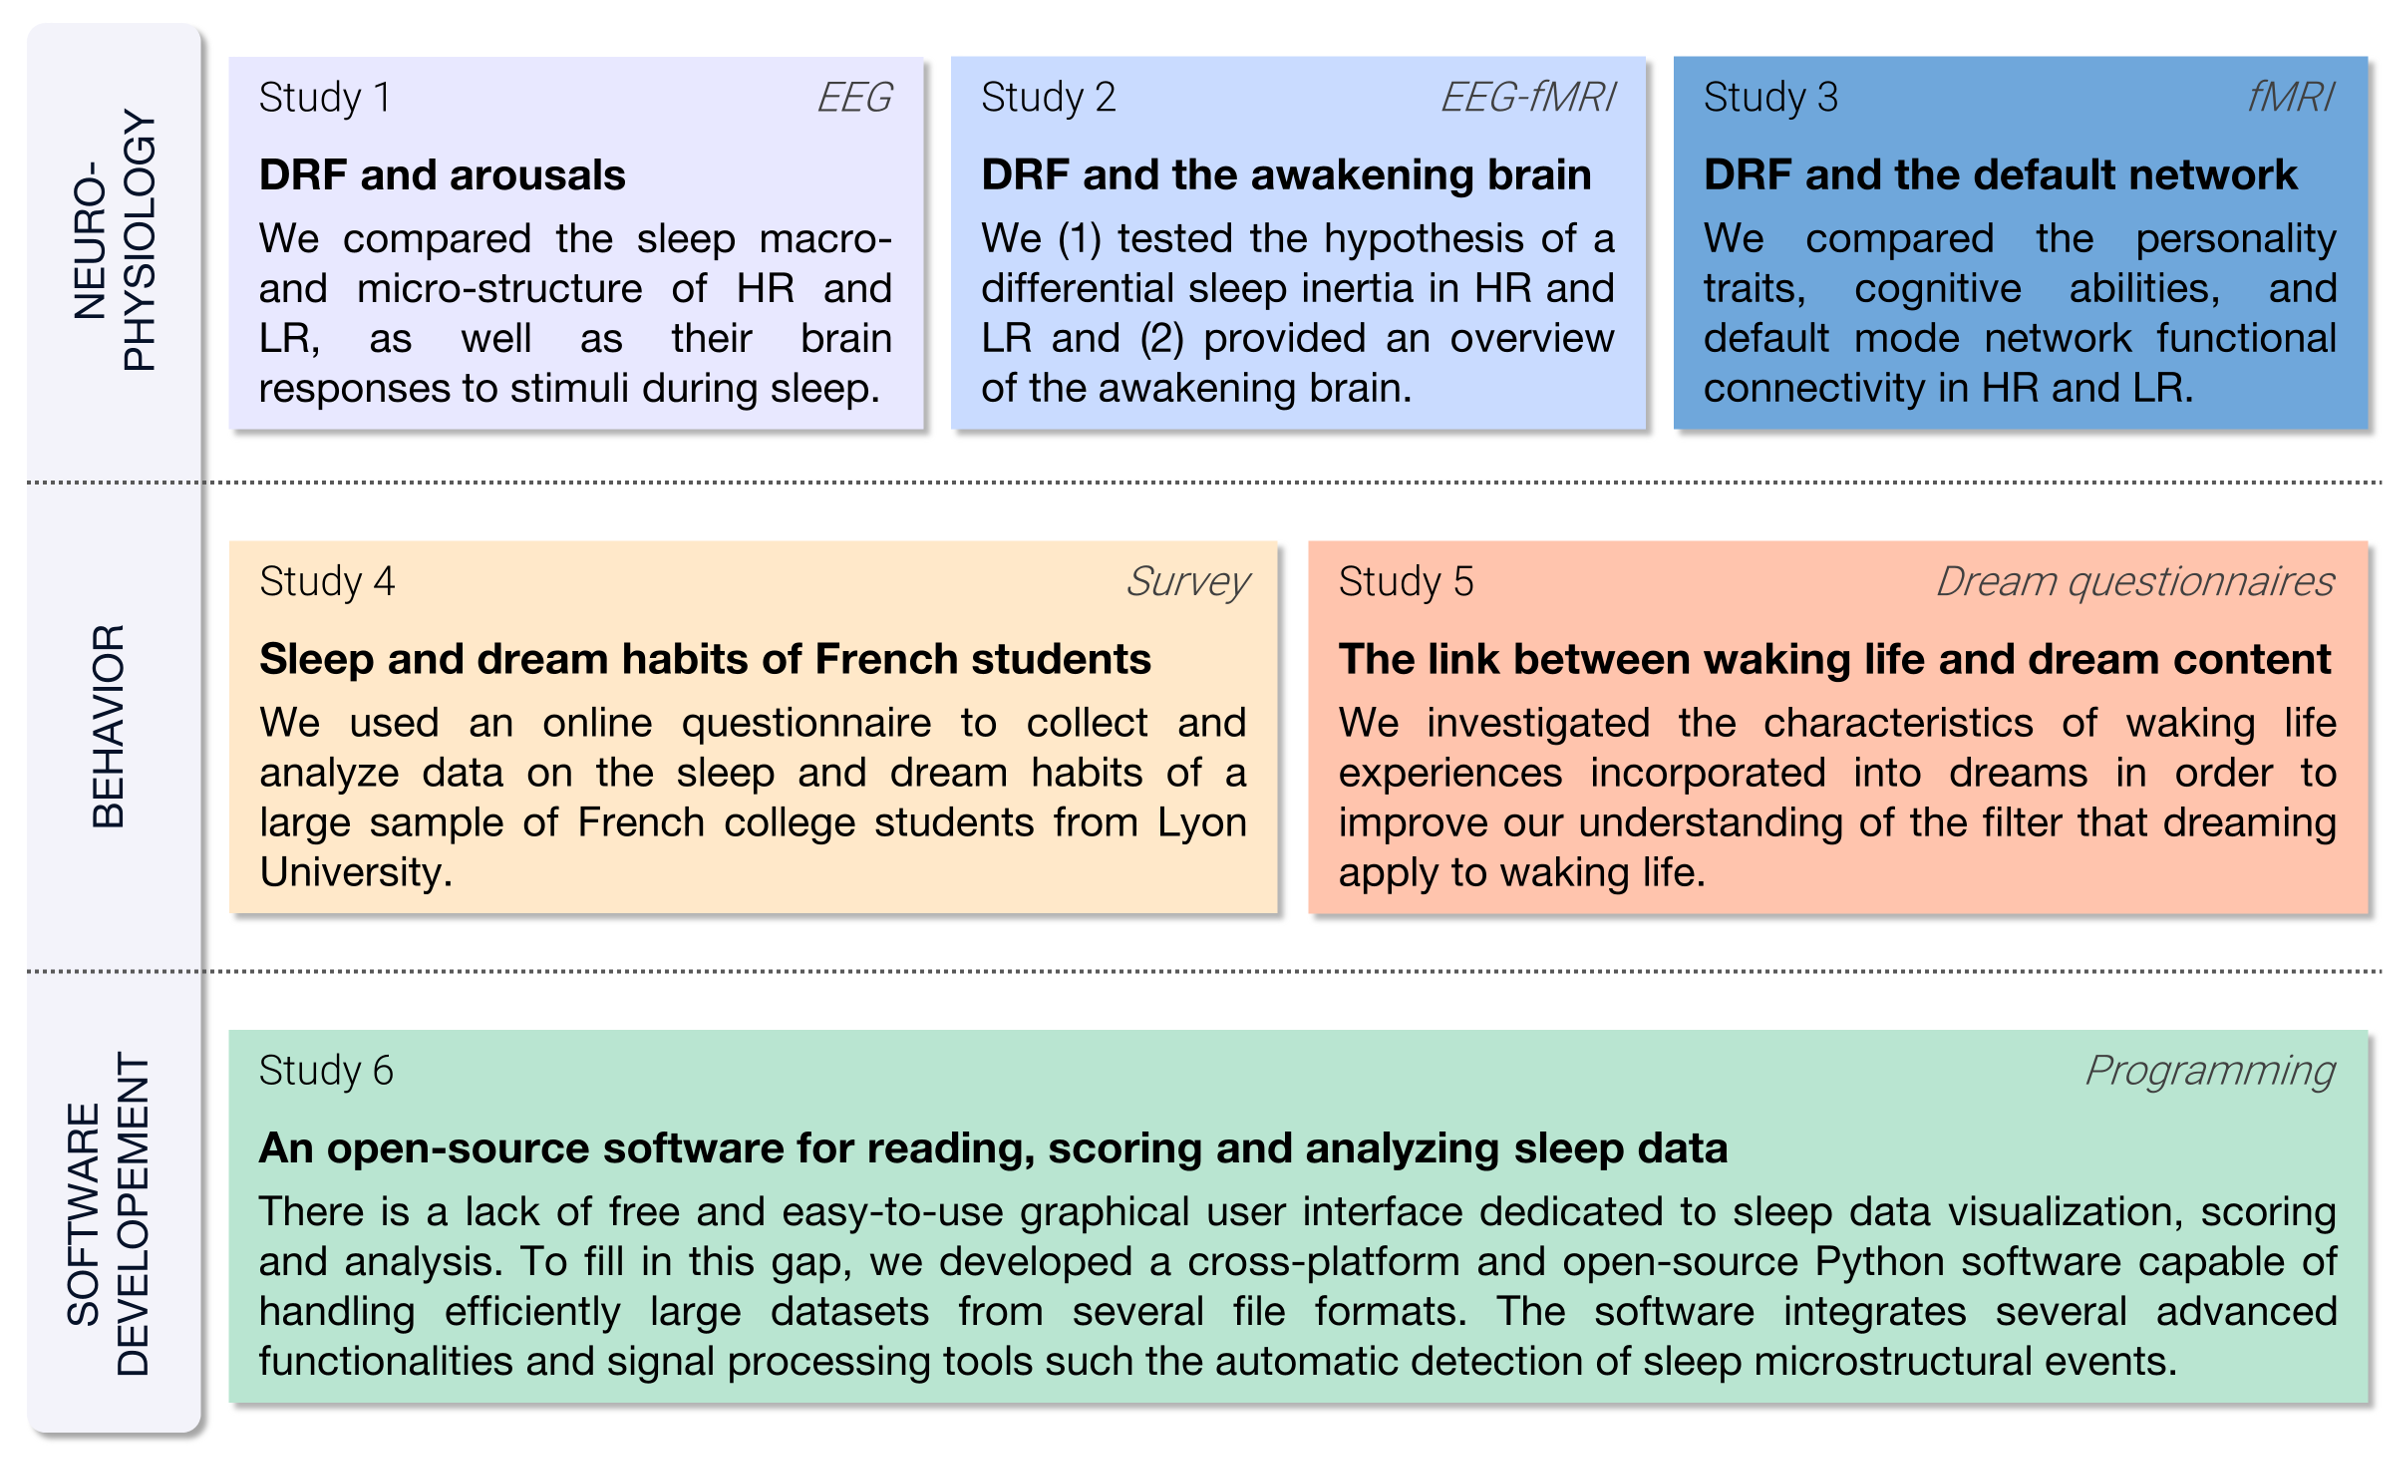
\includegraphics[width=\textwidth]{Fig/Intro/Intro_Problematics/Intro_Problematics.png}
	\caption[Summary of the studies conducted during my PhD thesis]{\textbf{Summary of the studies conducted during my PhD thesis}. In Studies 1, 2 and 3, we investigated the neurophysiological correlates of dream recall frequency (DRF), by comparing the sleep parameters, cognitive abilities and brain functional connectivity of high and low dream recallers (HR and LR respectively). Second, we used behavioral methods to collect data on the sleep and dream habits of college students (Study 4), as well as the relationship between waking life and dream content (Study 5). Finally, Study 6 relates to the ongoing development of an open-source software dedicated to sleep data.}
	\label{fig:intro:problematics-summary}
\end{figure}


% \part{METHODS}
% \cleardoublepage

\chapter{EEG and event-related potentials}
\label{sec:eeg}

\section{Electro-encephalography (EEG)}
\label{sec:eeg:eeg}

The first recording of the electric field of the human brain was made by the German psychiatrist Hans Berger in 1924. He named this recording electroencephalogram (EEG; \citealp{berger_uber_1929}). Since then, EEG and event-related potentials (ERP; see next section) have become one of the most prominent technique in research (e.g. neuroscience, psychology) and medical settings (e.g. epilepsy, sleep disorders). EEG records voltage fluctuations resulting from ionic current within large assemblies of neurons in the brain. The brain electrical activity is measured with electrodes that are placed either along the scalp or, in rarer circumstances, directly on the exposed surface of the brain (electro-corticography or intra-cranial EEG). Through the current thesis, we will focus solely on the former and non-invasive, scalp EEG method, which is also one of the three essential electrophysiological measurements of polysomnography, along with EOG and EMG (see section \ref{sec:dream-research:sleep:stages}).

\subsection{International 10-20 system}
\label{sec:eeg:eeg:10-20}

EEG is generally recorded from multiple electrodes distributed across the scalp. To allow reproducibility both within and between individuals, the placement of these electrodes is defined in the internationally standardized 10-20 system, which relies on the relationship between the location of an electrode and the underlying area of cerebral cortex (Figure \ref{fig:methods:10-20}). Electrode location are determined using two standard anatomical landmarks, the nasion and inion, respectively located between the eyes and at the back of the skull. From these points, the skull perimeters are measured in the transverse and median planes and electrode locations are determined by dividing these perimeters into 10\% and 20\% distance intervals. Electrodes names refer to their locations on the cerebral cortex. Thus, the first letter refers to the brain lobe on which they are located (F = frontal, C = central, P = parietal, O = occipital), while the number corresponds to the hemispheres (3 = left, 4 = right). For example, F3 is located on the left hemisphere of the frontal lobe, while P4 lies on the right hemisphere of the parietal lobe.

\begin{figure}[htb]
	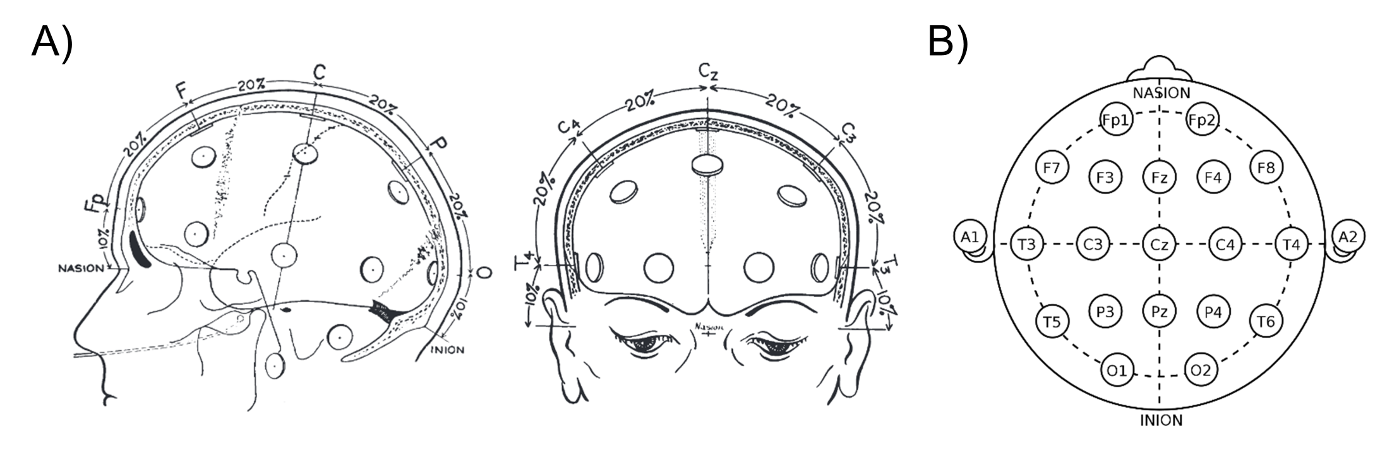
\includegraphics[width=\textwidth]{Fig/Methods/EEG_10-20/EEG_10-20.png}
	\caption[Electrode locations of International 10-20 system for EEG recording]{Electrode locations of International 10-20 system for EEG recording. (A) Lateral and frontal views of the skull showing the methods of measurement for electrode placement (adapted from \citealp{klem_ten-twenty_1999}). (B) Single plane projection of the head showing all standard positions and names of electrodes according to the 10-20 system. }
	\label{fig:methods:10-20}
\end{figure}

\subsection{Amplification, filtering and montage}
\label{sec:eeg:eeg:ampli}

The brain electrical activity is quite small (usually under 100 µV). For that reason, the EEG signal recorded on the scalp must be first amplified by several thousand times. In modern, digital EEG, the signal from each channel is then turned into a series of discrete digital values, with a sampling frequency generally comprised between 200 to 5000 Hz. The signal is then filtered and displayed on a computer screen using dedicated softwares such as Elan \citep{aguera_elan:_2011} or EEGLAB \citep{delorme_eeglab:_2004}. Typical filters include high-pass (<0.1 Hz), low-pass (35-70 Hz), and notch (50 or 60 Hz) to remove very slow artefacts, high-frequency artefacts (such as electromyographic activity) and electrical noise, respectively.
Since the EEG is measured as the voltage (i.e. potential for electrical charges to move between two locations) between two electrodes, the display of EEG may be set up in several ways, referred to as montage. In the standard, referential montage, a single reference electrode, located at a site thought to be electrically neutral, such as the earlobe or the mastoid, is typically used for all the active scalp electrodes. By contrast, in the average reference montage, the averaged signal across all electrodes is used as the common reference for each channel.

\subsection{Neural oscillations}
\label{sec:eeg:eeg:neural}

The spontaneous brain electrical activity is characterized by rhythmic oscillations, which are sometimes referred to as neural oscillations or, more popularly, as \q{brain waves}. These oscillations are generated by the summation of synchronous activity of thousands or millions or neurons (mainly cortical pyramidal neurons). They have characteristic frequency ranges, spatial distributions and are associated with different states of brain functioning (e.g. waking and the various sleep stages; see Figure \ref{fig:methods:neural}).

\begin{figure}[htb]
	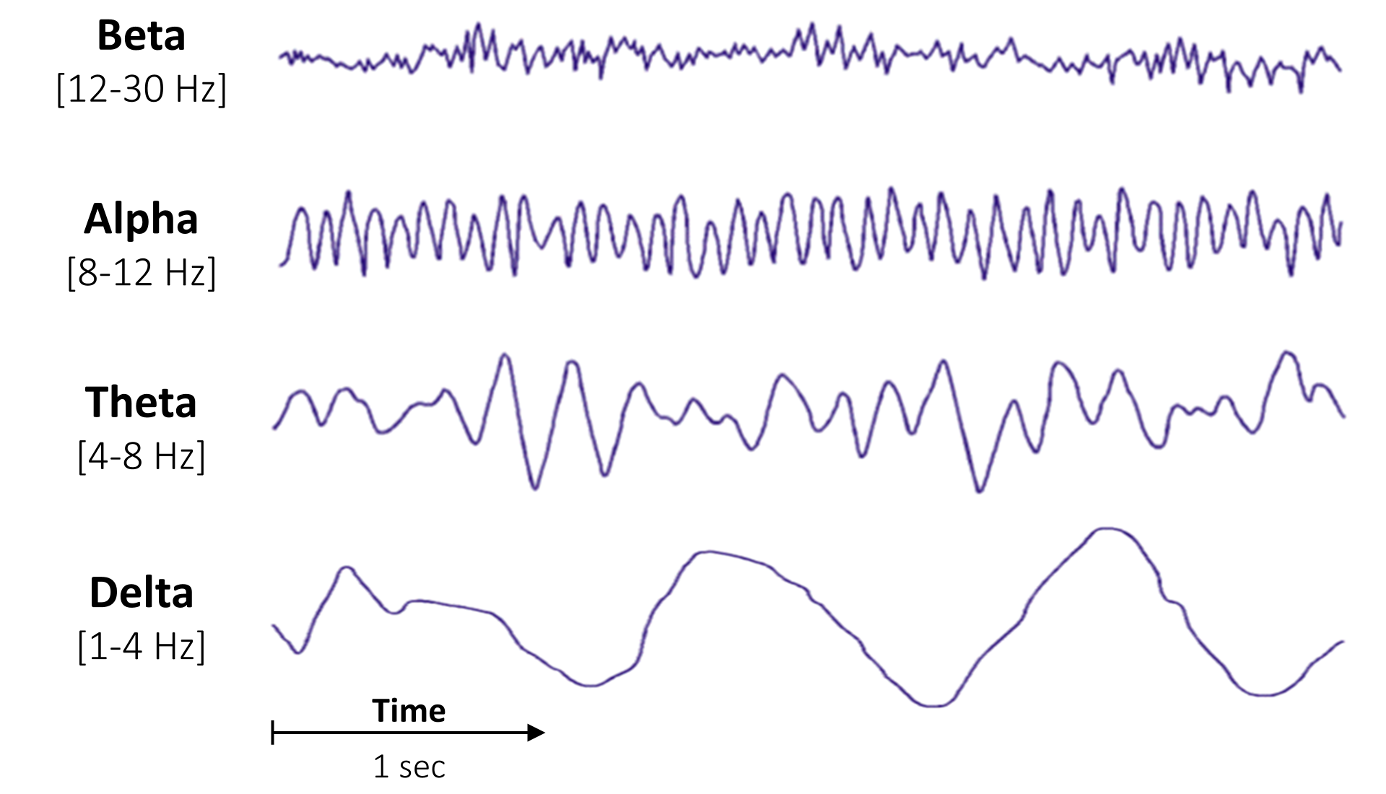
\includegraphics[width=\textwidth]{Fig/Methods/EEG_BrainWaves/EEG_Brain_Waves.png}
	\caption[Brain rhythms]{Brain rhythms. Beta waves are prominent over occipital and parietal areas during normal waking wakefulness. Alpha waves are prominent in occipital regions during eyes-closed wakefulness. Theta waves are detectable during N2 sleep and REM sleep. Delta waves are visible during N3 sleep (also called slow-wave sleep or deep sleep) and have a large amplitude (>75 µV) due to a high level of neural synchronization.}
	\label{fig:methods:neural}
\end{figure}

\section{Event-related potentials (ERP)}
\label{sec:eeg:erp}

\subsection{Definition and methods}
\label{sec:eeg:erp:def}

Event-related potentials (ERPs) are \q{electrical potentials generated by the brain that are related to specific internal or external events such as stimuli, responses or decisions} \citep{luck_introduction_2014}. A single ERP, usually recorded by means of scalp EEG, has an amplitude ranging from 0.5 to 15 µV, and is therefore much lower than the spontaneous background EEG (100 µV). As a consequence, a single ERP is not visible to the naked eye in the EEG signal. In order to disentangle and reveal the specific relevant ERP from the irrelevant background EEG, ERP technique relies on the mathematical principle of summation. It consists of averaging hundreds of time-locked repetitions of the same experimental condition in order to attenuate activities that are unrelated to the specific internal or external event.
The resulting waveform contains a series of positive and negative peaks (components) that are thought to reflect activity (i.e. postsynaptic potentials) in underlying generators within the brain. These components are usually referred to with acronyms (e.g. contingent negative variation, CNV) or by a letter indicating polarity (N = negative, P = positive), followed by a number indicating the latency in milliseconds from stimulus onset (e.g. N100 is a negative peak arising approximatively 100 ms after stimulus). Early components, which arise approximatively less than 80 ms after the stimulus, are thought to reflect sensory processes and are therefore intrinsically linked to the physical characteristics of the stimulus. By contrast, late components (>100ms) are thought to reflect more cognitive processes such as attention, memory and response preparation. They differ from the former in the sense that they are not systematically elicited but rather require the participant to be involved in some stimulus-related task (e.g. a detection task). While some potentials are easily obtain by repetition of stimuli (e.g. the N100 potential, elicited by perception of auditory stimuli), others potentials are elicited by more complex paradigm. One of the most famous is probably the oddball-paradigm, in which low-probability target (or \textit{deviant}) items are mixed with high-probability non-target (or \textit{standard}) items. Target items elicit a late positive component, the P300, though to reflect brain processes involved in stimulus evaluation or categorization.

\begin{figure}[htb]
	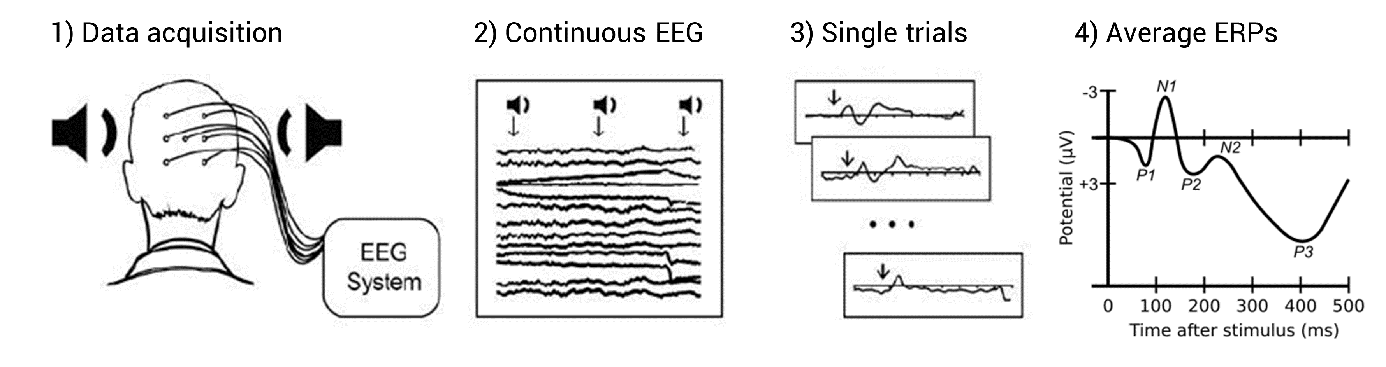
\includegraphics[width=\textwidth]{Fig/Methods/ERP/ERP.png}
	\caption[Schematic representation of ERP acquisition]{Schematic representation of ERP acquisition. (1) Scalp electrodes record electrical brain activity while auditory stimuli are presented repeatedly through headphones or speakers. (2) Stimulus onset/offset markers are recorded along with the continuous EEG signal. (3) Individual segments locked to stimulus onset are extracted from the continuous EEG and include a brief pre-stimulus baseline in addition to post-stimulus period of interest. (4) Averaged ERP waveform showing several components (including the N100 and P300) reflecting time- and phase-locked neural activity associated with stimulus processing. Note that the ERP is plotted with negative voltages upward, a common, but not universal, practice in ERP research. Adapted from \citet{key_human_2016}}
	\label{fig:methods:erp}
\end{figure}

\subsection{The use of ERP in sleep research}
\label{sec:eeg:erp:erp}

ERP is a method of choice for the investigation of the normal and pathological human sleep \citep{bastuji_evoked_1999, colrain_use_2007}. One reason for this is that it allows to study objectively information processing during sleep, limited otherwise by the lack of the ability of subjects to make verbal or motor responses to stimuli. It provides a powerful, objective and non-invasive means to study for example the extent of sensory integration during sleep, or the neurological abnormalities related to sleep disorders, or sleep inertia upon waking \citep{bastuji_event-related_2003}.
ERP studies greatly improved our understanding of sleep, from the classical view that sleep is a “little death” (illustrated by the fraternal link between Hypnos, God of Sleep, and Thanatos, God of Death, in the Greek mythology; see \citealp{mazza_asleep_2014}), to the emerging idea that sleep is a dynamic process in which complex cognitive processing occur \citep{andrillon_sleeping_2016}. For example, a P300 component has been observed during REM sleep in response to target stimuli presented within an oddball paradigm \citep{bastuji_brain_1995}. Similarly, there is a persistence of the brain’s ability to detect semantic incongruity during REM sleep  (N400; \citealp{perrin_detection_2002}).
It should however be noted that considerable differences exist between waking, NREM and REM sleep ERP components \citep{bastuji_evoked_1999, colrain_use_2007}. Specifically, while early sensory components (i.e. peripheral and brainstem responses) remain unaffected by the sleep cycle, early cortical responses are drastically modified, in part because the thalamus stops relaying sensory information to the brain. Finally, late cortical responses displays profound changes during NREM sleep, which revert in REM sleep.

% \cleardoublepage

\chapter{fMRI and functional connectivity }
\label{sec:fmri}

\section{Structural and functional magnetic resonance imaging}
\label{sec:fmri:fmri}

\subsection{Magnetic resonance imaging (MRI)}
\label{sec:fmri:fmri:mri}

Magnetic resonance imaging (MRI) is probably the \q{most important imaging advance since the introduction of X-rays by Conrad Röntgen in 1895} \citep{logothetis_what_2008}. It is undoubtedly true that the emergence of MRI has indeed marked the beginning of a new era in diagnostic medicine and basic research. MRI is based upon nuclear magnetic resonance, the physical phenomenon by which nuclei placed in an external magnetic field absorb and re-emit radio-frequency energy. MRI is the technique of choice for imaging brain structure, in part because magnetic properties of hydrogen nuclei vary with the biological tissue in which they are. Consequently, the rate of spin relaxation (i.e. how quickly spins \emph{forget} the direction in which they are oriented) is not the same between gray and white matter, which thus makes it possible to construct detailed images of the brain at any location and orientation with sub-millimeter resolution.

\subsection{Functional MRI (fMRI)}
\label{sec:fmri:fmri:fmri}

Functional MRI (fMRI), built on the earlier concept of MRI, is a technique for measuring hemodynamic changes (i.e. blood flow dynamic) in the brain due to changing neural activity. Compared to structural MRI, the brain is scanned at lower spatial resolution (2-3 mm) but at a higher temporal resolution (typically a few seconds). Specifically, fMRI relies on the fact that hemoglobin in blood slightly distorts the magnetic resonance properties of hydrogen nuclei in its vicinity, and the amount of magnetic distortion changes depending on whether the hemoglobin has oxygen bound to it. For example, when neurons of a specific brain area become active, local blood flow to this region increase, and oxygen-rich (oxygenated) blood displaces oxygen-depleted (deoxygenated) blood around 2 seconds later (a phenomenon known as the hemodynamic response). These changes in the concentration of oxygen and blood flow lead to localized blood oxygenation level-dependent (BOLD) changes in the magnetic resonance signal. It is generally accepted that, in most brain regions, the fMRI signal is coupled to the level of excitatory and inhibitory synaptic transmission and therefore reflect the level of information processing \citep{logothetis_what_2008}.

\subsection{Task-based and resting-state paradigms}
\label{sec:fmri:fmri:paradigm}

Traditionally, fMRI has been used to produce maps of task-dependent brain function using block or event-related designs, which are based on the subtraction paradigm. In such designs, one infers the level of activation of certain brain areas by looking at the relative changes from baseline (resting or control condition) in the BOLD signal during the performance of a task or in response to a stimulus. During these designs, participants are instructed to perform specific tasks, which are generally designed to target a single brain function such as vision, attention, memory, emotion recognition and so on. These paradigms have allowed brain science to take giant strides, in particular on the issue of linking brain areas with specific functions (which was in the past only possible by studying cerebral lesions).

More recently, there has been a growing interest in the application of resting-state fMRI (RS-fMRI). Indeed, soon after the development of fMRI, some researchers observed that the resting brain was not silent but contained information about its functional organization \citep{biswal_functional_1995}. Specifically, they reported that, during rest, time courses of low frequency fluctuations (<0.1 Hz) in somatomotor brain areas, showed a high degree of temporal correlation. They argued that this correlation, which may arise from fluctuations in blood oxygenation or flow, is a manifestation of functional connectivity of the brain. Although at the time Biswal’s seminal observation was mostly disregarded, it laid the basis for the now widely-used resting-state fMRI paradigm, which measures how different regions of the brain communicate while participants are not performing any active task. Although both resting-state and task-related designs measures BOLD signal, there are several major differences between the two, which are reported in Table \ref{tab:method:fMRI-paradigm}.

\begin{table}[htb]
    \centering
    \caption[Key differences between task-based fMRI and resting-state fMRI]{\textbf{Key differences between task-based fMRI and resting-state fMRI}. Modified from \citet{smitha_resting_2017}}
    \label{tab:method:fMRI-paradigm}
    \begin{tabularx}{\textwidth}{lXX}
    \toprule
                          & Task-based fMRI                                                                                                 & Resting-state fMRI                                                                   \\ \midrule
    Design                & Analyses of the relative changes from baseline in the BOLD signal during a task or in response to a stimulus    & Analyses of the spontaneous BOLD signal in the absence of any explicit task or input \\
    Energy consumption    & Task-specific increase in neuronal metabolism are less than 5\%                                                 & 60–80\% of brain’s energy is consumed during resting state                           \\
    Brain areas           & The focus is only on a very small fraction of the brain’s overall activity                                      & The focus is on large-scale brain networks                                           \\
    Signal-to-noise ratio & Low since 80\% of the BOLD modulation is discarded as noise                                                     & Good since it takes the overall spontaneous low frequency fluctuations               \\
    Patient cooperation   & Patient cooperation is essential                                                                                & Pediatric, psychiatric and comatose patients can do it                               \\
    Duration              & Requires a large number of repetitions                                                                          & Usually 6 to 10 minutes                                                              \\ \bottomrule
    \end{tabularx}%
\end{table}

\section{Functional connectivity}
\label{sec:fmri:fc}

\subsection{Overview}
\label{sec:fmri:fc:overview}

Functional connectivity can be defined as \q{the temporal dependence of neuronal activity patterns of anatomically separated brain regions} \citep{van_den_heuvel_exploring_2010}. It can be measured as long-range synchronization of the EEG, magneto-encephalography (MEG), or other dynamic brain signals. Applied to fMRI, functional connectivity reflects the temporal correlation of low frequency (<1 Hz) BOLD spontaneous fluctuations in spatially distinct brain regions (Fig \ref{fig:methods:fcmri}). Although the true neuronal basis of these slow BOLD fluctuations is not yet fully understood, there is converging evidence that they result from co-activation in the underlying spontaneous neuronal activation patterns. As a consequence, they are thought to reflect functional communication between brain areas. There are also several evidences that spontaneous BOLD fluctuations are partly constrained by anatomic connectivity \citep{van_dijk_intrinsic_2010}.

In more practical terms, these intrinsic BOLD fluctuations are nearly always measured at rest in order to minimize task-evoked effect. Resting-state fMRI has also the advantage of being quite simple to implement. For that reason, functional connectivity resting-state MRI has become the technique of choice to study the intrinsic functional organization of the brain in healthy individuals across a variety of vigilance states (such as sleep) but also in patients (e.g. comatose and psychiatric patients).

\begin{figure}[htb]
	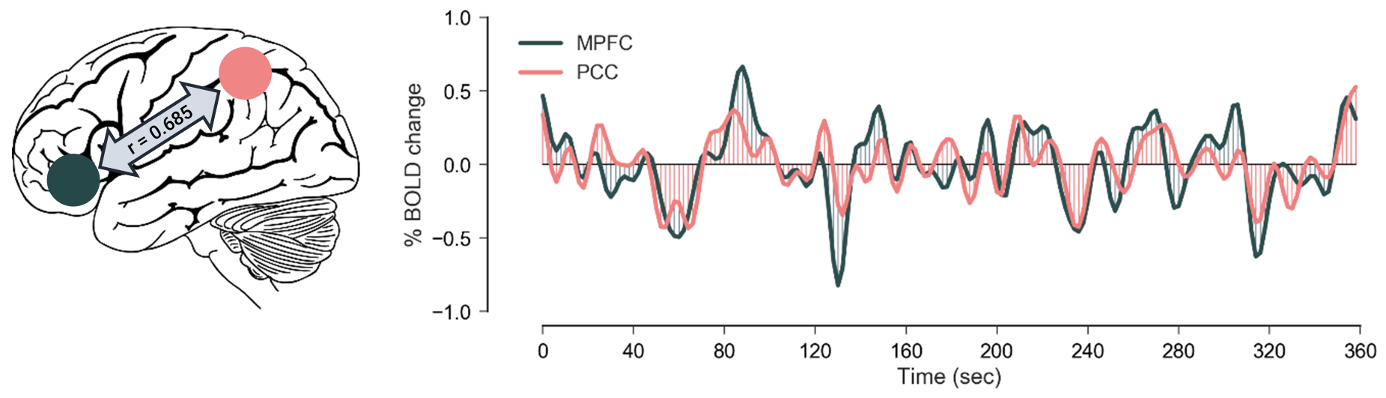
\includegraphics[width=\textwidth]{Fig/Methods/fMRI_temporal_correlation/fMRI_temporal_correlation.png}
	\caption[The basic strategy of functional connectivity MRI]{\textbf{The basic strategy of functional connectivity MRI}. The basis of functional connectivity is that spontaneous BOLD fluctuations measured at rest are correlated between spatially distinct brain regions. In this example, spontaneous BOLD fluctuations in the medial prefrontal cortex (MPFC) and posterior cingulate cortex (PCC) are correlated (Pearson r = 0.685). These data come from a 6-min resting state scan acquired in a single individual on a 3-tesla MRI scanner.}
	\label{fig:methods:fcmri}
\end{figure}

\subsection{Large-scale brain networks}
\label{sec:fmri:fc:network}

A decade of resting-state fMRI research has revealed that the human brain is organized into several large-scale functionally-correlated brain networks, which are consistently found in healthy subjects, different stages of consciousness and across species \citep{fox_spontaneous_2007, yeo_organization_2011}. Because they are preferentially identified during resting-state fMRI, these networks are often referred to as resting-state networks. They are comprised of different brain regions that each have their own task and function, but which are continuously exchanging information with each other. Remarkably, they closely match the topographies of functional responses obtained by task-related fMRI using typical sensory, motor, and cognitive paradigms.
The main functional networks of the human brain are depicted in Fig \ref{fig:methods:networks}. The visual and somatomotor networks include regions of the primary and secondary visual and sensory-motor cortex respectively. These two sensory networks are characterized by a clear coupling between anatomic and functional connectivity \citep{van_dijk_intrinsic_2010}. Next, come the so-called task-positive networks, namely the frontoparietal (FP; sometimes referred to as executive, or control) network, the dorsal attention network (DAN), and the salience network. They are all involved in attentional processes. For instance, the DAN is thought to support selective attention to sensory features of the environment, while the salience network is involved in monitoring the salience of external inputs and internal brain events. There is emerging evidence that the FP network, originally thought to be involved in the selection of sensory contents by attention, may also orchestrate the interactions between other networks \citep{christoff_mind-wandering_2016}.

\begin{figure}[htb]
    \centering
	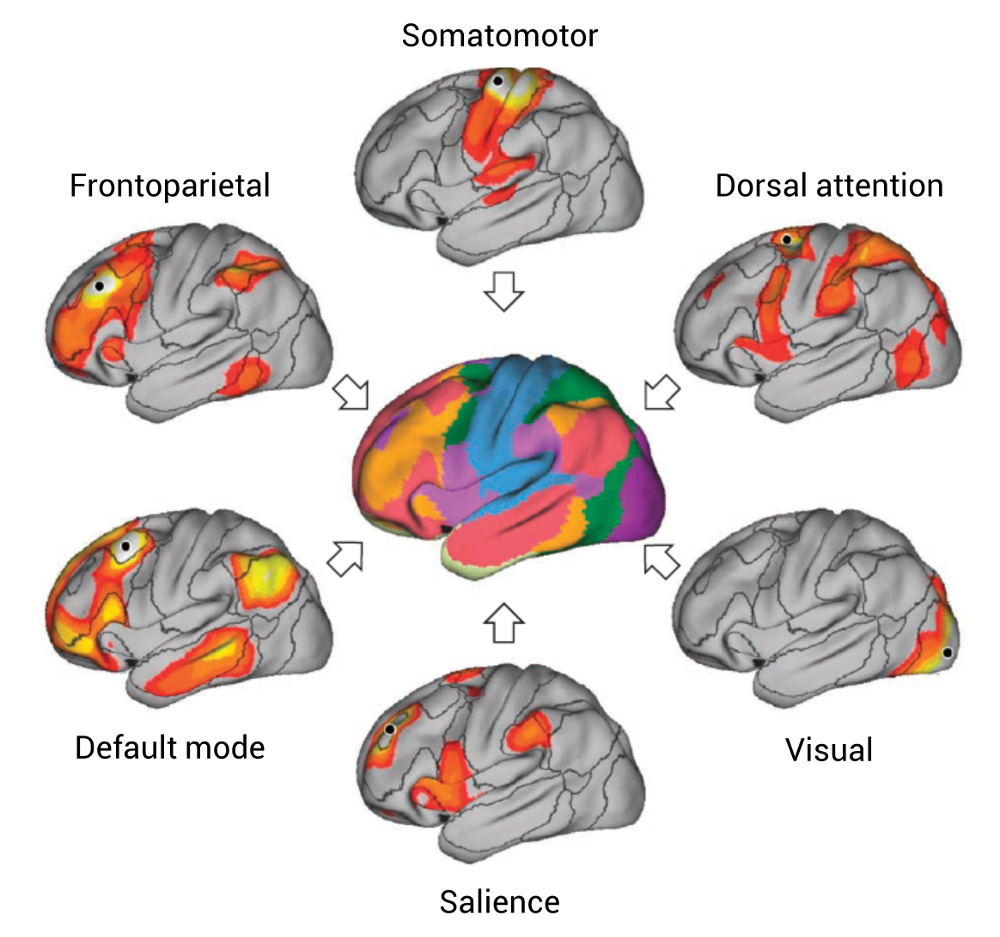
\includegraphics[width=0.9\textwidth]{Fig/Methods/fMRI_Networks/fMRI_Networks.png}
	\caption[Large-scale brain networks]{\textbf{Large-scale brain networks identified with resting-state functional connectivity fMRI}. Outer maps show the functional connectivity maps for a single seed region (black circle) placed in a different cortical region, obtained using resting-state fMRI data in 1000 subjects. Center map shows a composite estimate of the networks using an analytical approach to parcellate cortical regions into their most dominant network. Originally published in \citet{buckner_opportunities_2013}}
	\label{fig:methods:networks}
\end{figure}

Finally, the last and perhaps most investigated brain network is the default mode network (DMN, sometimes referred to as task-negative network), which was originally identified as a set of brain areas consistently deactivated across a range of externally oriented tasks \citep{raichle_default_2001}. It has been linked to internal mental processes, such as introspection, mind-wandering but also episodic memory retrieval and autobiographical future thinking. The DMN includes several subsystems which are supposedly involved in different functional roles  (Fig \ref{fig:methods:dmn}; \citealp{andrews-hanna_functional-anatomic_2010}). The DMN is probably one of the more robust brain network, and it has been identified across several vigilance states, including NREM and REM sleep \citep{horovitz_decoupling_2009, larson-prior_cortical_2009, larson-prior_modulation_2011, wu_variations_2012}. Recently, some authors have postulated that the DMN might be involved in the production and/or encoding of dreams (see section \ref{sec:dream-research:attempts:dmn}).

\begin{figure}[htb]
    \centering
	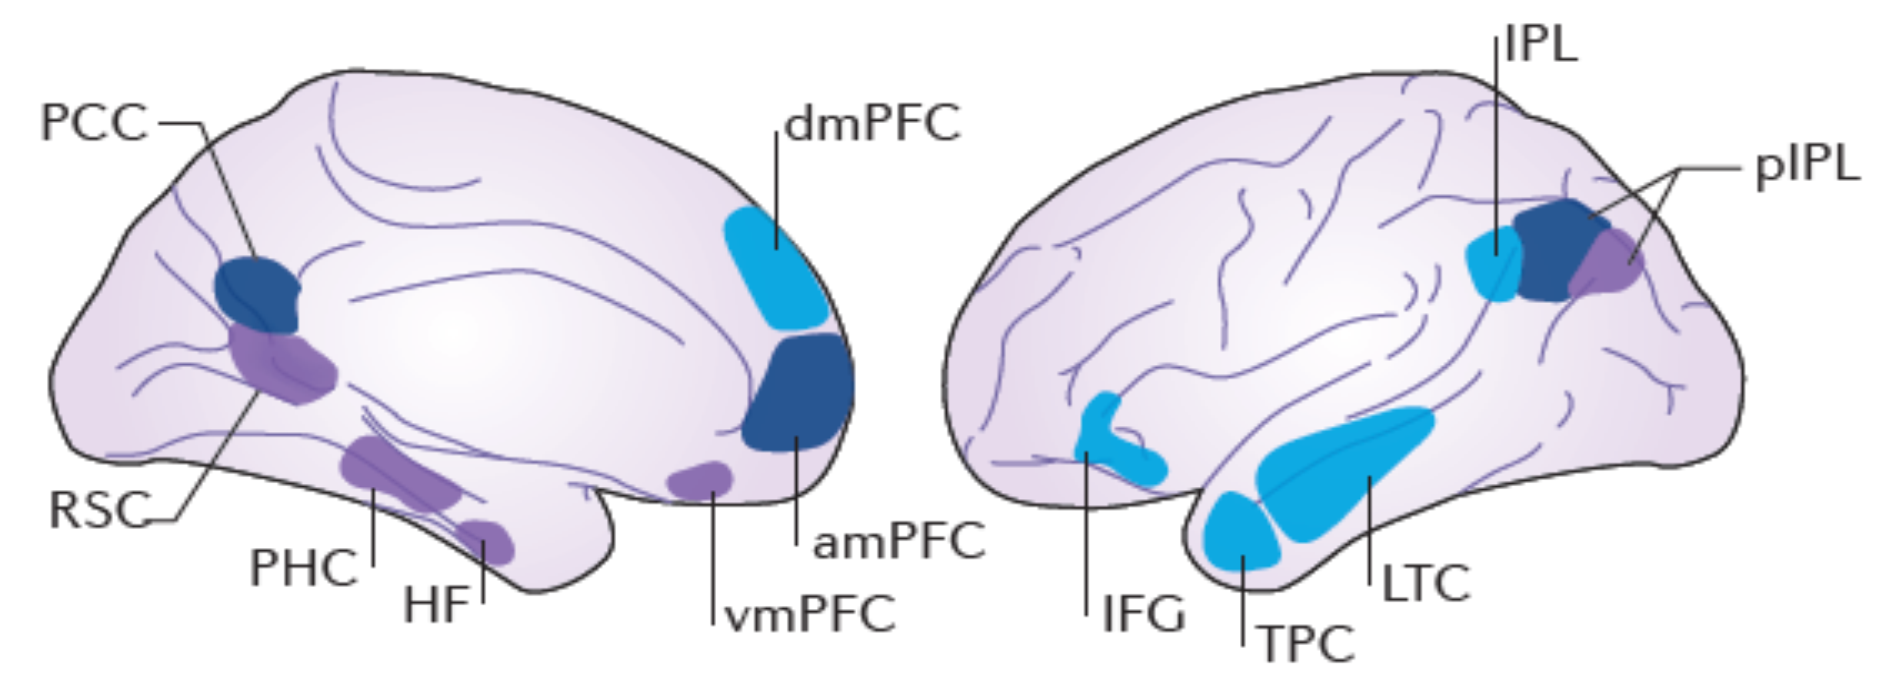
\includegraphics[width=0.9\textwidth]{Fig/Methods/fMRI_DMN/Intro_DMN.png}
	\caption[The default mode network and its subcomponents]{\textbf{The default mode network and its subcomponents}. The DMN is centered on the medial prefrontal cortex (MPFC), the medial parietal cortex and the lateral parietal cortex, and extends into the temporal lobe and lateral prefrontal cortex. Three subcomponents within the DMN have been identified. The first, the core DMN subsystem (deep blue) includes the MPFC, posterior cingulate cortex (PCC) and posterior inferior parietal lobule (pIPL). It is characterized by its hub-like properties and its contributions to internally oriented cognition. The second subcomponent (purple), which is known for its roles in memory and mental simulation, is centered on the medial temporal lobe (MTL), and includes as well the hippocampal formation (HF) and parahippocampal cortex (PHC). The third subcomponent (cyan) extends more dorsally and includes the dorsomedial prefrontal cortex (dmPFC), the lateral temporal cortex (LTC), the temporopolar cortex (TPC) and parts of the inferior frontal gyrus (IFG). It seems to be linked to a wide range of functions, including mentalizing, conceptual processing and emotional processing. Originally published in \citet{christoff_mind-wandering_2016}.}
	\label{fig:methods:dmn}
\end{figure}

\subsection{Anti-correlations between networks}
\label{sec:fmri:fc:anti-correl}

\citet{fox_human_2005} reported that the DMN is negatively coupled (anti-correlated) to brain networks involved in focused external visual attention (i.e. mainly the DAN). In other words, when the spontaneous BOLD fluctuations increase in the DMN, they decrease in the DAN. This dynamic interplay between two large, spatially distributed networks representing a priori opposing components of our mental lives (the DMN is involved in internal mental processes, while the DAN is involved in external attention) may \q{mark a fundamental feature of brain organization that had not been appreciated by earlier techniques} \citep{buckner_opportunities_2013}. Remarkably, a decrease anti-correlation between the DMN and the DAN has been consistently reported in a variety of altered vigilance states such as during NREM sleep (review in \citealp{picchioni_sleep_2013}) and after total sleep deprivation \citep{de_havas_sleep_2012}. This suggests that anti-correlation between these networks is an essential part of the brain normal functional organization.

\section{Resting-state fMRI data analysis}
\label{sec:fmri:rs}

The aim of this section is to provide a brief overview of the numerous processing steps that must be performed to go from the raw structural and functional MRI images to the group-level statistical analysis. These steps are summarized in Fig \ref{fig:methods:fmri-pipeline}.

\subsection{Preprocessing}
\label{sec:fmri:rs:preproc}

Steps in the spatial preprocessing of task-related and resting state fMRI data are similar. The first step is usually slice-timing correction, which aims at correcting temporal offset between slices within a repetition time by applying a temporal data interpolation to each voxel of the brain. Indeed, an fMRI scanner typically requires 2 seconds (i.e. repetition time or TR) to construct a full 3D brain volume by slicing the brain into multiple 2D layers (acquired either in ascending or interleaved order). Consequently, the BOLD signal (hemodynamic response) acquired in the last slice (late in the TR) peaks earlier than those in the slices acquired early in TR, even though the underlying activity is identical. Slice-timing correction applies a temporal data interpolation to each voxel of the brain in order to reconstruct a signal as if all the slices within a TR were acquired at the same exact time point.
The second main step is the coregistration which refers to the alignment of functional and structural images from the same subject to map functional information into anatomical space. In layman’s term, this step ensures that the brain images acquired from a single individual are always in the same position and space. This step is particularly important in resting-state fMRI due to the global effect of head movements on spontaneous BOLD fluctuations.
Next comes normalization, which refers to the spatial transformation of individual brains into a common space (typically Montreal Neurological Institute (MNI) space), a step crucial in order to make brain volumes acquired in different subject with different brain morphologies comparable to each other. A temporal filtering is sometimes applied to remove or attenuate frequencies within the raw signal that are not of interest. For instance, as functional connectivity fMRI studies the spontaneous low-frequency BOLD fluctuations, a bandpass filter on frequencies between 0.01 Hz - 0.1 Hz is usually applied. Finally, the last preprocessing step is generally the spatial smoothing, which aims at further increasing the signal-to-noise ratio by filtering out high frequency regions. Smoothing is a prerequisite to parametric statistical analysis (such as the Gaussian random fields) which assume that data are well-modeled by a normal distribution, however, there is a controversy as to the role of smoothing in resting-state fMRI (and notably graph analysis) in which increased spatial dependency introduced by smoothing might confound local connectivity strength \citep{hayasaka_comparison_2010}.

\begin{figure}[!htb]
	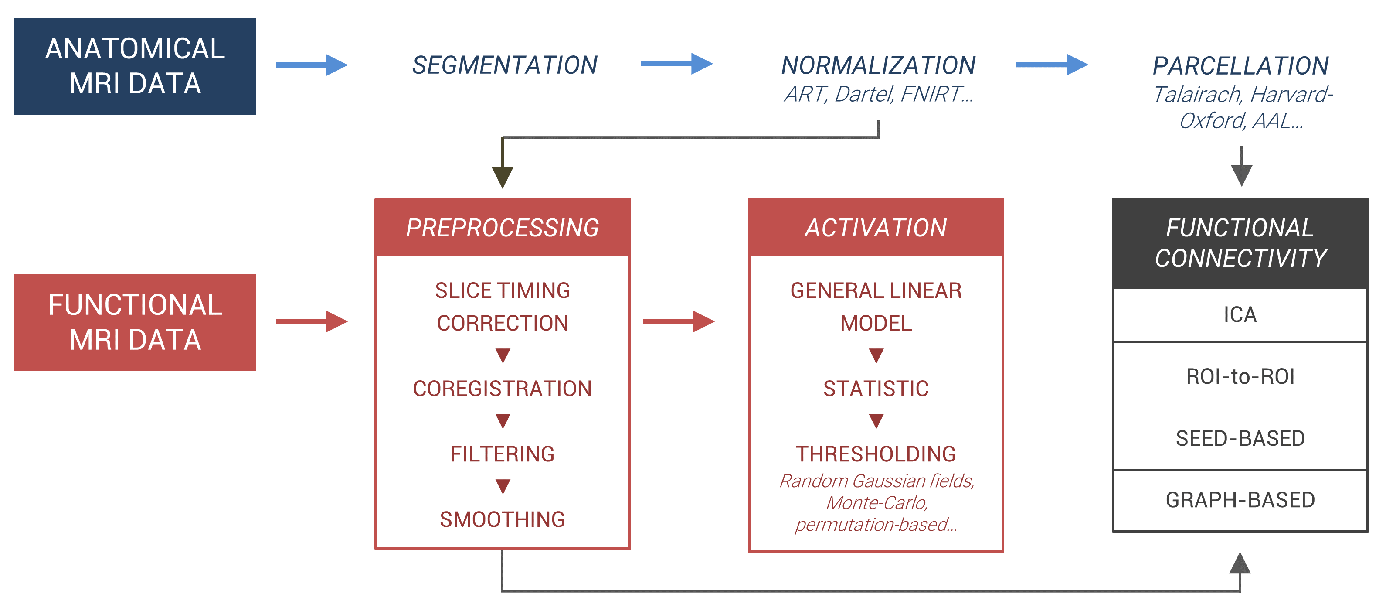
\includegraphics[width=\textwidth]{Fig/Methods/fMRI_pipeline/fMRI_pipeline_perso.png}
	\caption[Overview of the fMRI processing pipeline]{\textbf{Overview of the fMRI processing pipeline}. ICA = independent component analysis, ROI = regions of interests. Adapted from an original idea of Oussama Abdoun.}
	\label{fig:methods:fmri-pipeline}
\end{figure}

\subsection{Functional connectivity analysis}
\label{sec:fmri:rs:analysis}

There are three prominent methods to analyze preprocessed resting-state fMRI data (Fig \ref{fig:methods:ana-methods}). The first one is independent component analysis (ICA), which is a statistical method for separating a multivariate signal into additive subcomponents. Applied to brain functional connectivity data, it allows for example to separate distinct brain networks, without making any kind of initial assumptions \citep{beckmann_investigations_2005}. Because it requires no a priori defined regions of interests (ROIs), it can be quite easily implemented to identify brain networks or to remove noisy components of the signal (e.g. physiological noise, scanner drift). The second approach is based on a priori defined cluster of voxels (referred to as seeds, or ROIs). In this case, the signal from a specific seed is correlated either with all the other voxels of the brain (voxel-to-voxel approach) or others ROI (ROI-to-ROI approach). The ROI-to-ROI method is particularly well-suited to analyze within and between networks interactions, provided that the ROIs are defined a priori (for example using an ICA or a brain atlas). Finally, an emerging method in resting-state fMRI analysis is graph theory, which studies the spatio-temporal properties of brain networks using mathematical tools \citep{bullmore_complex_2009}.

\begin{figure}[htb]
	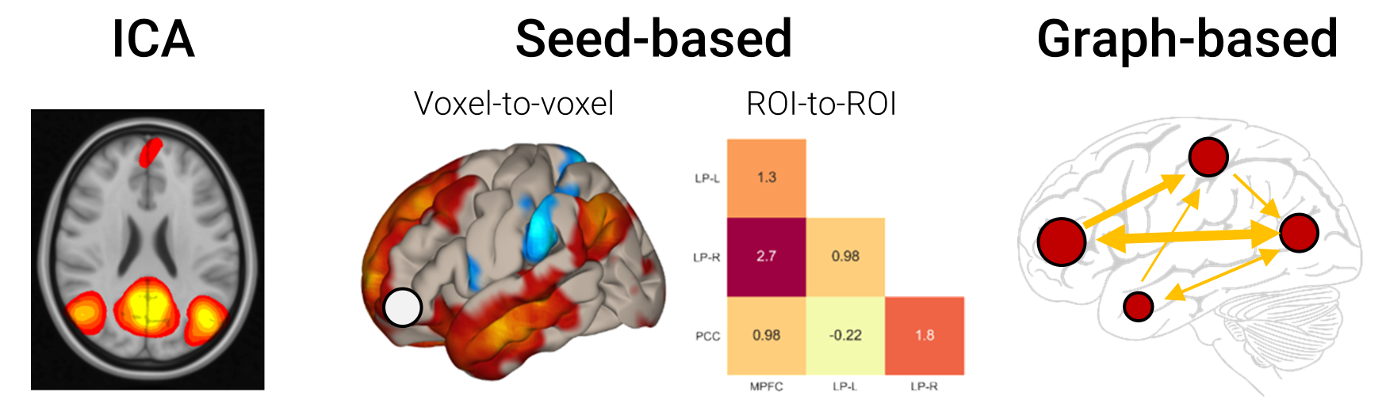
\includegraphics[width=\textwidth]{Fig/Methods/fMRI_seed_graph_ica/fMRI_seed_graph_ica.png}
	\caption[The three main methods of resting-state fMRI data analysis]{\textbf{The three main methods of resting-state fMRI data analysis}. (1) ICA is a highly data-driven method which is typically used to identify brain networks (in this example, the core regions of the DMN) or remove noisy components. (2) Seed-based connectivity requires one or several regions of interests (ROIs) to be a priori defined in order to compute the correlations between the seed regions and all the others voxels in the brain (voxel-to-voxel) or between specific ROIs (ROI-to-ROI). In this example, a symmetric correlation matrix was obtained by computing all the pairwise correlations within the DMN. (3) Graph-based connectivity studies the topological features of brain networks, which are defined in this context as a set of nodes (ROIs) linked by connections (edges). Using mathematical tools, several parameters can be computed such as the global efficiency and the level of modularity / clustering.}
	\label{fig:methods:ana-methods}
\end{figure}

\subsection{Combined EEG-fMRI recordings}
\label{sec:fmri:rs:eeg-fmri}

Simultaneous recording of EEG and MRI allow researchers to benefit from the excellent temporal resolution of EEG combined with the high spatial accuracy of fMRI. Applied to sleep, it allows for example to perform correlation between sleep features (detected using classic EEG-based criteria), and BOLD-fMRI signal \citep{duyn_eeg-fmri_2012}. The EEG can also be used to detect online the different sleep stages, thus allowing the experimenter to decide when to launch an fMRI scan. Simultaneous EEG-fMRI is therefore a valuable tool for investigating brain function across the spectrum of vigilance states.
However, there are a number of technical challenges that need to be overcome in order to improve EEG-fMRI data acquisition. Most importantly, EEG signals acquired during simultaneous fMRI are affected by several artefacts, namely the gradient artefact (caused by the changing magnetic fields gradients required for fMRI) and the cardio-ballistic artefact (linked to cardiac pulsations). Fortunately, these artefacts can be almost entirely removed, a posteriori but also in real-time, using dedicated softwares or algorithms.

%
% \cleardoublepage
% \part{EXPERIMENTAL RESULTS}
% % !TEX root = ../thesis-example.tex
%
\chapter{The role of arousals on DRF variability}
\label{res:arousal}

\cleardoublepage

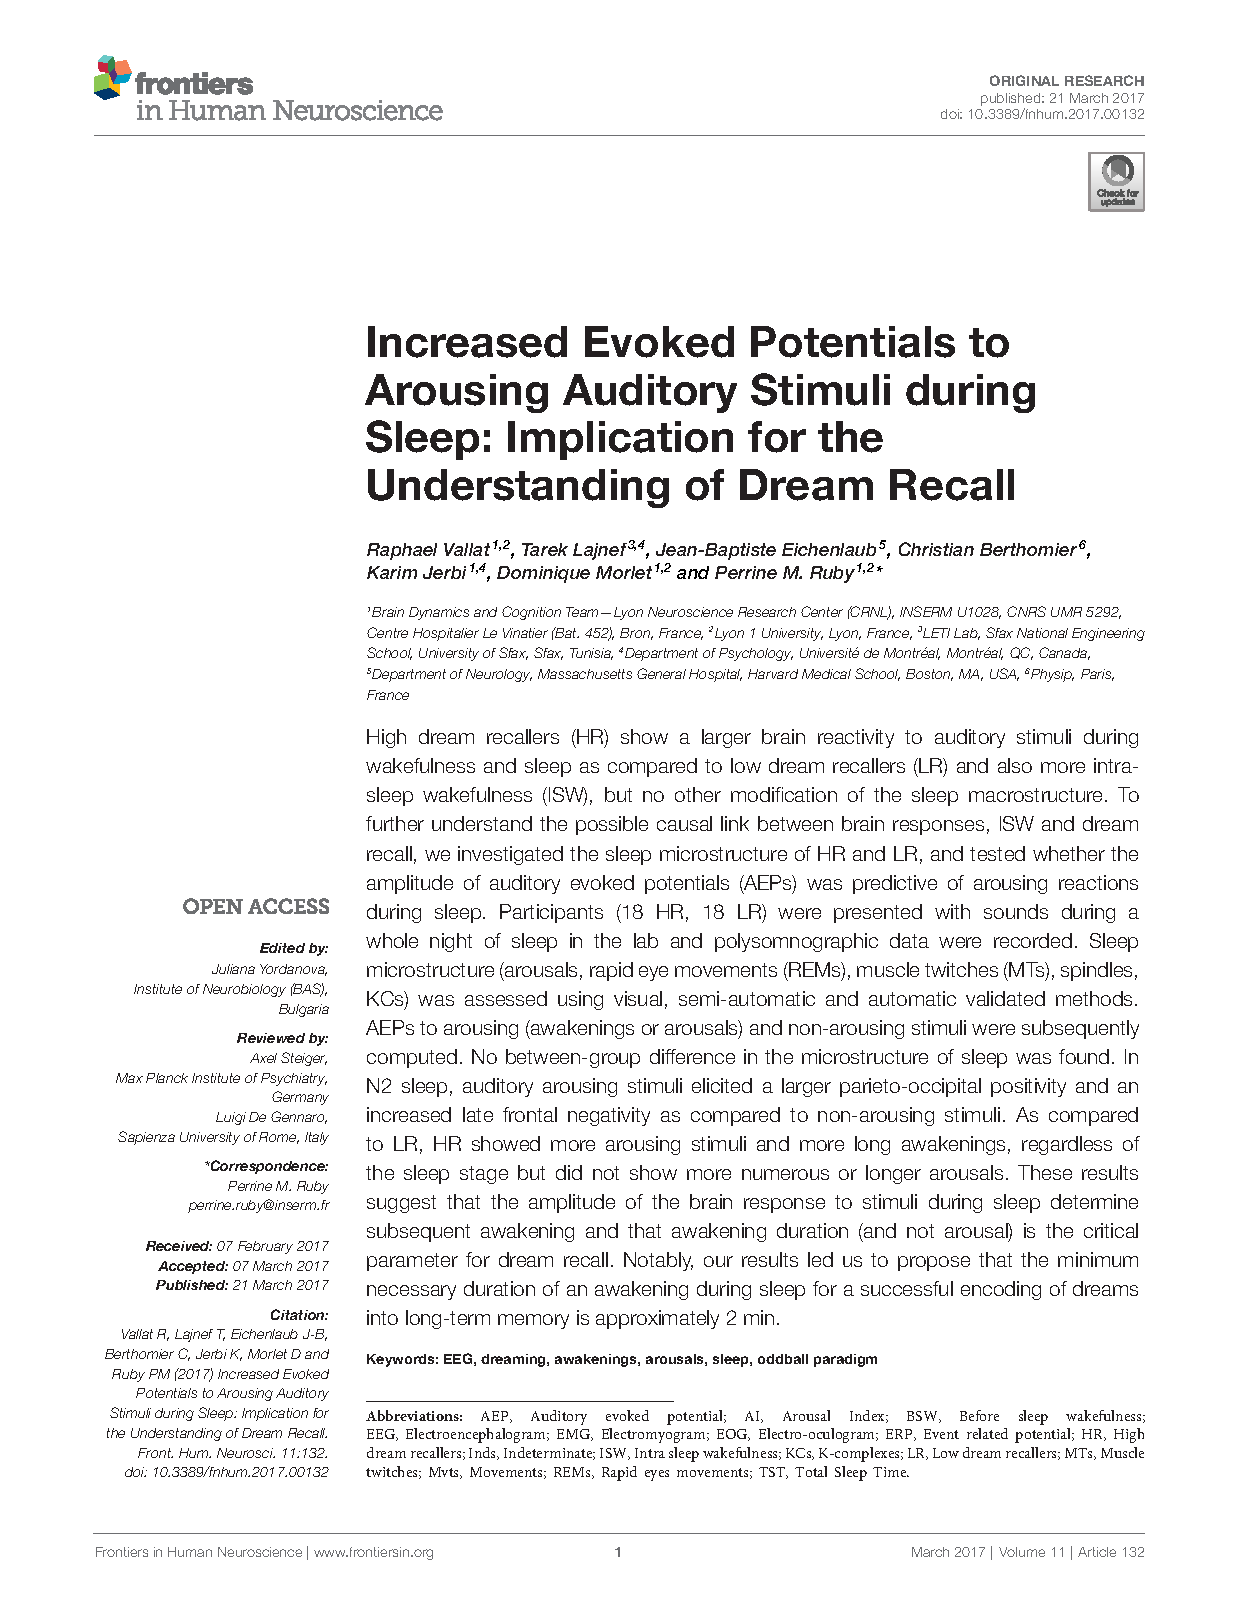
\includepdf[pages=-, pagecommand={\thispagestyle{plain}}]{Articles/Vallat_2017_FHN.pdf}

%
% \cleardoublepage
% \part{GENERAL DISCUSSION}

\cleardoublepage
% --------------------------
% Back matter
% --------------------------
\part{REFERENCES} \cleardoublepage
{
\setstretch{1.1}
\renewcommand{\bibfont}{\normalfont\small}
\setlength{\biblabelsep}{0pt}
\setlength{\bibitemsep}{0.5\baselineskip plus 0.5\baselineskip}
\printbibliography[nottype=online, heading=bibnumbered]
%\printbibliography[heading=subbibliography,title={Website},type=online,prefixnumbers={@}]
}

\cleardoublepage
% !TEX root = ../thesis-example.tex
%
\pagestyle{empty}
\hfill
\vfill
%\pdfbookmark[0]{Colophon}{Colophon}
\section*{Colophon}

This thesis was typeset with \LaTeXe.
It uses the \textit{Clean Thesis} style developed by Ricardo Langner.
The design of the \textit{Clean Thesis} style is inspired by user guide documents from Apple Inc.

Download the \textit{Clean Thesis} style at \url{http://cleanthesis.der-ric.de/}.


% **************************************************
% End of Document CONTENT
% **************************************************
\cleardoublepage
\end{document}
